\documentclass[final]{ukthesis}
%you must include these 2 packages.
\usepackage[pdfauthor={Michael A-P Brown},
            pdftitle={The UCNA Experiment: Analysis of the 2011-2013 Data},
            pdfsubject={The Subject},
            pdfkeywords={Some Keywords},
            pdfproducer={Latex with hyperref},
            pdfcreator={latex->dvips->ps2pdf},
            pdfpagemode=UseOutlines,
            bookmarksopen=true,
            bookmarksnumbered=true]{hyperref}
\usepackage{memhfixc}
\usepackage{graphicx}
\usepackage{amsmath}
%\usepackage[small]{titlesec}
%\setcounter{secnumdepth}{4}
\setcounter{tocdepth}{3}

%\changetocdepth{3}
%\maxsecnumdepth{subsection}
\setsecnumdepth{subsubsection}


\usepackage[
backend=bibtex,
style=alphabetic,
%sorting=ynt
]{biblatex}
\addbibresource{references}


%%%%%%%%%%%%%%%%%%%%%%%%%%%%%%%%%%%%%%%%%%%%%%%%
\begin{document}
%author data
\author{Michael A-P Brown}
\title{The UCNA Experiment: Analysis of the 2011-2013 Data}
\abstract{
  The UCNA Experiment at the Los Alamos Neutron Science Center (LANSCE) is the first measurement
  of the $\beta$-decay asymmetry parameter $A_0$ using polarized ultracold neutrons (UCN). $A_0$,
  which represents the parity-violating angular correlation between the direction of the initial
  neutron spin and the emitted decay electron's momentum, determines $\lambda=g_{A}/g_{V}$, the ratio
  of the weak axial-vector and vector coupling constants. A high-precision determination of
  $\lambda$ is important for weak interaction physics, and when combined with the neutron lifetime
  it permits an extraction of the CKM matrix element $V_{ud}$ solely from neutron decay. At LANSCE,
  UCN are produced in a pulsed, spallation driven solid deuterium source and then polarized via
  transport through a 7 T magnetic field. Their spins can then be flipped via transport through
  an Adiabatic Fast Passage spin flipper located in a low-field-gradient 1 T field region prior
  to transport to a decay storage volume situated within a 1 T solenoidal spectrometer. Electron
  detector packages located at each end provide for the measurement of decay electrons. Previous
  UCNA results (based on data collected in 2010 and earlier) were limited by systematic
  uncertainties, in particular those from the UCN polarization, calibration of the electron
  energy, and electron backscattering. This dissertation will present a background of Neutron
  Decay, an overview of the UCNA Experiment, followed by a detailed report on the entire analysis
  process for the 2011/2012 and 2012/2013 data sets.}

\advisor{Dr. Bradley Plaster}
\keywords{UCN,Neutrons}
\dgs{Dr. Tim Gorringe}
%the title pages
\frontmatter
\maketitle


\begin{acknowledgments}
  The friendship and guidance provided by Dr. Brad Plaster made this work possible. I thank you.
  Also to Dr. Renee Fatemi, Dr. Susan Gardner, and Dr. Kevin Donohue, I thank you for serving on
  my dissertation committee and seeing this process through.
\end{acknowledgments}


\begin{dedication}
  This work is dedicated to my parents, Cindy and John, and my soon-to-be wife, Kirstie, for their
  unending support. And also to Piper, my four-legged friend who keeps me sane.
\end{dedication}


\tableofcontents\clearpage
\listoffigures\clearpage
\listoftables\clearpage

%----------------------------------------------

\mainmatter
\OnehalfSpacing

% Chapter 1
\chapter{Introduction}
\label{ch:Introduction}

The purpose of this dissertation is to describe in detail
the methods used in extracting the $\beta$-decay asymmetry parameter
for the UCNA Experiment. This chapter hopes to motivate the inception
of the parameter of interest and its role in the theory of $\beta$-decay.
Also introduced are characteristics of the neutron itself with an
emphasis on ultracold neutrons (UCN), the namesake of the UCNA experiment.

%%%%%%%%%%%%%%%%%%%%%%%%%%%%%%%%%%%%%%%%%%%%%%%%%%%%%%%%%%%%%%%%%%%%%%%%%%%%%%%
%%%%%%%%%%%%%%%%%%%%%%%%%%%%%%%%%%%%%%%%%%%%%%%%%%%%%%%%%%%%%%%%%%%%%%%%%%%%%%%

\section{The Standard Model}
The Standard Model of particle physics encompasses everything we know about
interactions between particles and describes nature using the most fundamental
building blocks yet discovered. This section is used as an introduction
to these building blocks, the quarks and leptons, and to the mediators of the
interactions between them, to preface the upcoming descriptions of the neutron
and $\beta$-decay.

\subsection{The Building Blocks}

\subsection{The Forces}

\subsection{Symmetries}



%%%%%%%%%%%%%%%%%%%%%%%%%%%%%%%%%%%%%%%%%%%%%%%%%%%%%%%%%%%%%%%%%%%%%%%%%%%%%%%
%%%%%%%%%%%%%%%%%%%%%%%%%%%%%%%%%%%%%%%%%%%%%%%%%%%%%%%%%%%%%%%%%%%%%%%%%%%%%%%

\section{Properties of the neutron}
\label{sec:neutronProperties}
Let us take a moment to give a very brief introduction to the neutron to motivate the
upcoming sections. This will also serve as a useful tool for those who are
unfamiliar with nuclear and field theories, as the following sections become
quite technical. The majority of this dissertation can be read and mostly understood
without much knowledge of the theoretical description behind neutron $\beta$-decay,
so the properties of the neutron are a natural starting point.

The neutron is a net neutrally charged composite particle. The terms net and
composite hint at the inner structure of the neutron, made up of fundamental
particles called quarks, in this case two down ($d$) quarks and one up ($u$) quark.
The quarks do carry charge, with the $u$ charge $+2/3$ and the $d$ charge
$-1/3$, so that the net charge of the neutron is zero. This can be compared
to the proton, another composite particle made up of three quarks (two $u$ and
one $d$ quark), whose net charge is $+1$ and the other nucleon found
within a nucleaus along with the neutron. Four other quarks exist,
the charm, strange, bottom, and top in order of increasing mass. The neutron
is the second lightest three-quark composite particle (baryon) 
behind only the proton.

The free neutron undergoes $\beta$-decay, defined as a transition from the neutron
to a proton, electron, and electron anti-neutrino,
\begin{equation*}
  n\rightarrow p + e^- + \bar{\nu}_{e}.
\end{equation*}
\noindent The three-body decay gives rise to a continuous energy spectrum
for the proton, electron, and anti-neutrino by conservation of energy and momentum
as seen in figure \ref{fig:spectralShapes}. The lifetime of the free neutron is
approximately fifteen minutes.


\section{$\beta$-decay of the neutron}

Prior to 1930, $\beta$-decay of nuclei was a polarizing topic of debate. Originally
only the decay electron was detected, and given such a two-body decay (the recoil
nucleus and the emitted electron being the two bodies) one would expect a discrete
electron energy defined by the difference in mass between mother and daughter
nuclei. Instead, a continuous energy spectrum was observed for the electron, which
initially led some to believe that energy conservation was moot. Others, like
Wolfgang Pauli, were not ready
to abandon energy conservation. He postulated that a neutral particle
could also be emitted in the decay. This third particle would share the energy available
in the reaction, explain the continuous energy distribution of the electron, and go
on undetected as it would not interact electromagnetically. The particle was termed
the neutrino by Fermi, and it would be a crux of Fermi's theory of $\beta$-decay.
A quarter century later, the existence of the neutrino would be confirmed
experimentally \cite{cowan1956detection}.

\subsection{Fermi's Theory of $\beta$-decay}
After Pauli postulated the existence of the neutrino to explain the continuous energy
distribution of the $\beta$-decay electron, Fermi attempted to theoretically describe
the process in a similar manner to the theory of emission of
gamma radiation from an excited nucleus \cite{fermi1934,wilson1968fermi}.
His theory relied on two postulates: the existence of the neutrino and that the nucleus consisted
of heavy particles only, the neutron and the proton, both of which would turn out to be true.

\begin{table}[h]
  \caption{Transformation behavior of all possible bilinear covariants.} 
  \centering
  \begin{tabular}{l c }
    \hline \hline \\ [-1.75ex]
    $\bar{\psi}\psi$ & scalar \\ [0.50ex]
    $\bar{\psi}\gamma^5\psi$ & pseudoscalar \\ [0.50ex]
    $\bar{\psi}\gamma^{\mu}\psi$ & vector \\ [0.50ex]
    $\bar{\psi}\gamma^{\mu}\gamma^5\psi$ & axial vector \\ [0.50ex]
    $\bar{\psi}\sigma^{\mu\nu}\psi$ & antisymmetric tensor \\ [0.50ex]   
    \hline
  \end{tabular}
  \label{tab:bilinearCov}
\end{table}

Fermi's Hamiltonian took the form (written in a different manner from Fermi's original
paper on the subject for the sake of clarity) 
%
\begin{equation}
  H = C_V\big( \bar{\psi}_p \gamma_\mu \psi_n \big) \big( \bar{\psi}_e \gamma^\mu \psi_\nu \big), 
\end{equation}
%
where $\bar{\psi} \gamma_\mu \psi$ is a vector current (see table \ref{tab:bilinearCov}). The assumption
that the current-current interaction would be of the vector-vector variety was a natural
choice as this is the case for electromagnetism.

\begin{figure}
  \centering
  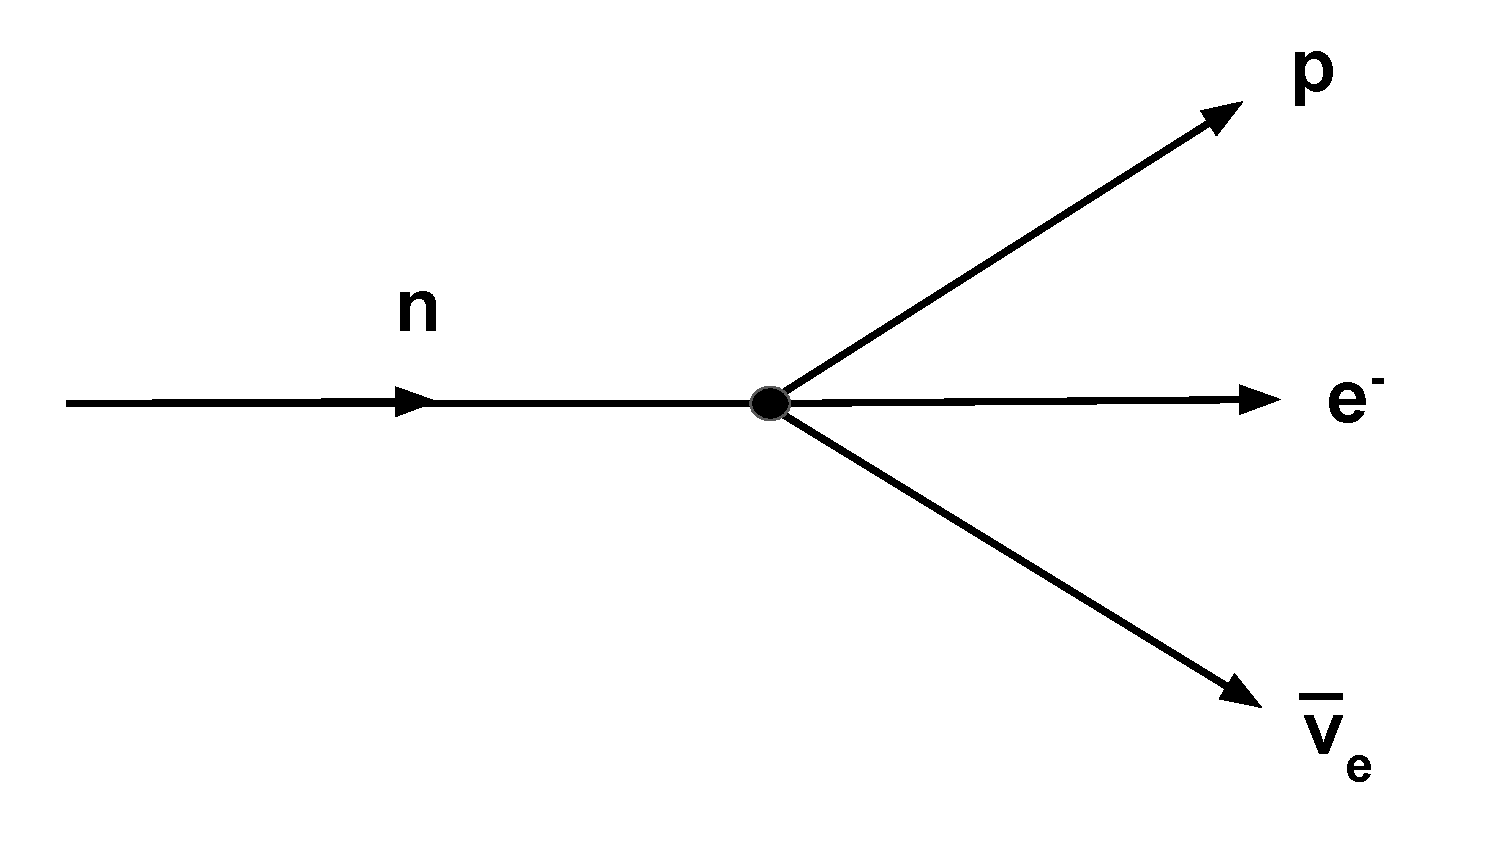
\includegraphics[scale=0.50]{1-Introduction/pointInteraction.pdf}  
  \caption{The point interaction of Fermi's theory of $\beta$-decay. The theory is
    capable of describing other processes which move one of the outgoing particle lines
    to the left side, like electron capture by the proton producing a neutron and an
    electron neutrino.}
  \label{fig:pointInteraction}
\end{figure}

Fermi's theory of $\beta$-decay treats the decay as a four-point contact interaction
(see figure \ref{fig:pointInteraction}), where
the currents are evaluated at the same point in space and time \cite{renton1990}. For those
familiar with quantum field theory within the Standard Model, this differs from the typical
interaction Hamiltonian as there is no propagator, or force carrier, to mediate the
interaction between the two currents (more on this later). The theory
worked well at predicting the energy spectrum of the electron from which
Fermi deduced that the neutrino must be nearly massless, but suffered one flaw. The vector
nature of the theory did not permit the observed allowed nuclear $\beta$-decay transitions
which can transform the spin of the decaying nucleus. This was pointed out by Gamow and Teller in
1936 \cite{gamow1936}, where they show that a current-current interaction that transforms like
a pseudovector properly assigns the spins of the products in thorium decays. As such,
one can generalize Fermi's theory by including all possible bilinear covariant terms that
satisfy both Lorentz and translational invariance:
%
\begin{multline}
  H = C_S\big( \bar{\psi}_p \psi_n \big) \big( \bar{\psi}_e  \psi_\nu \big) 
  +C_V\big( \bar{\psi}_p \gamma_\mu \psi_n \big) \big( \bar{\psi}_e \gamma^\mu \psi_\nu \big) \\
  +C_T\big( \bar{\psi}_p \sigma^{\mu\nu} \psi_n \big) \big( \bar{\psi}_e \sigma^{\mu\nu} \psi_\nu \big) 
  +C_A\big( \bar{\psi}_p \gamma_\mu \gamma^5 \psi_n \big) \big( \bar{\psi}_e \gamma^\mu \gamma^5 \psi_\nu \big) 
  +C_P\big( \bar{\psi}_p  \gamma^5 \psi_n \big) \big( \bar{\psi}_e  \gamma^5 \psi_\nu \big),
\end{multline}
%
where the coefficients quantify the coupling to each respective current.

This shortcoming of Fermi's original vector-vector interaction
lends itself to the definition of
two types of allowed $\beta$-decay transitions. The Fermi transition proceeds through the
scalar and vector currents with $\Delta J=0$ and no parity change. Gamow-Teller transitions
correspond to the axial vector and tensor currents and have $\Delta J=0,\pm1$ with no parity change,
but excluding the $0^+\rightarrow 0^+$ nuclear transitions. The pseudoscalar terms does not
contribute to the amplitude in the low energy limit \cite{renton1990}.
 

\subsection{Parity Violation in Weak Decays}

\subsubsection{Lee and Yang}

Prior to the 1950's, all discrete symmetries (parity, charge conjugation, and time reversal)
were thought to be conserved separately for all interactions in nature. A dilemma arose when
two particles, called the $\tau$ and $\theta$ mesons at the time, posessed the same mass
and charge as the $K^+$ meson, but decayed to different final states of parity. The $\tau$ decayed into three pions
and the $\theta$ into two pions. The initial classification of the two observably identical particles into
two different particles was logical given that parity conservation was then sacrosanct,
but in 1956 Lee and Yang proposed a very different solution to the problem. They realized that
there was no evidence that parity must be conserved in the weak interaction.
In the full expression of Fermi's theory (equation \ref{eq:FermiFull}),
while including all possible combinations of bilinear covariants, there was no mixing between the
individual currents and each individual current-current term transforms like a scalar. For example,
two individual axial vector currents would each transform as
$P(\bar{\psi}_p \gamma_\mu \gamma^5 \psi_n) \rightarrow -\bar{\psi}_p \gamma_\mu \gamma^5 \psi_n$ under parity, but the
muliplication of two such terms transforms like a scalar. Thus, none of the terms in \ref{eq:FermiFull})
are capable of violating parity, as the Hamiltonian would remain invariant. 

In their 1956 paper \cite{leeyang1956}, Lee and Yang modified the weak ineraction Hamiltonian
by including the possibility of a pseudoscalar current-current interaction, namely
%
\begin{multline}
  H = \bar{\psi}_p \psi_n \big( C_S\bar{\psi}_e  \psi_\nu + C'_S\bar{\psi}_e \gamma^5 \psi_\nu \big) \\
  + \bar{\psi}_p \gamma_\mu \psi_n  \big( C_V\bar{\psi}_e \gamma^\mu \psi_\nu + C'_V\bar{\psi}_e \gamma^\mu \gamma^5 \psi_\nu \big) 
  + \bar{\psi}_p \sigma^{\mu\nu} \psi_n \big( C_T\bar{\psi}_e \sigma^{\mu\nu} \psi_\nu + C'_T\bar{\psi}_e \sigma^{\mu\nu} \gamma^5 \psi_\nu \big)\\
  + \bar{\psi}_p \gamma_\mu \gamma^5 \psi_n \big( C_A\bar{\psi}_e \gamma^\mu \gamma^5 \psi_\nu + C'_A\bar{\psi}_e \gamma^\mu \psi_\nu \big) 
  + \bar{\psi}_p  \gamma^5 \psi_n \big( C_P\bar{\psi}_e  \gamma^5 \psi_\nu + C'_P\bar{\psi}_e \psi_\nu \big).
  \label{eq:leeyang}
\end{multline}
%
If any of the $C'_i$ coefficents are nonzero, parity would not be conserved due to
the scalar-pseudoscalar form of the current-current interactions that are labelled by
the primed coefficients.

Along with the inclusion of potential parity violating terms in the Hamiltonian, Lee and Yang
presented several potential tests of parity violation in the weak sector. One such proposition
was the measurement of the correlation between the spin of a polarized nucleus and
the momentum of the $\beta$-decay electron.

\subsubsection{Discovery of Parity Violation}

Following the publication of Lee and Yang's newly modified theory of $\beta$-decay, C. S. Wu
and collaborators designed an experiment \cite{wu1957} to test the potential violation
of parity in the $\beta$-decay of $^{60}\mathrm{Co}$
($^{60}\mathrm{Co} \rightarrow {^{60}\mathrm{Ni}} + e^- + \bar{\nu}_e$). The premise of the experiment
was simple: place an electron detector along the $+z$ axis, polarize the $^{60}\mathrm{Co}$ nuclei
using a magnetic field in the $\pm z$ direction, and measure the electron rate in each polarization
configuration. If parity is violated, a clear asymmetry would be present between the two polarizations,
which is precisely what was discovered and can be seen in figure \ref{fig:wuData}.

\begin{figure}[h]
  \centering
  \includegraphics[scale=0.50]{1-Introduction/wuData.png}  
  \caption{Data from C. S. Wu's experiment measuring the correlation between the emitted
    direction of the electron from the decay of polarized $^{60}\mathrm{Co}$. The two
    curves represent the counting rates when the nuclei were oriented in opposite
    directions with respect to the electron detector. The existence of a splitting
    indicatesa violation of parity as the electrons are preferentially emitted in the
    direction opposite the spin.}
  \label{fig:wuData}
\end{figure}

The measurement showed that the electrons were preferentially
emitted in the direction opposite the spin of the nuclei, which indicates parity violation due to
the position inverted scenario not being observable. This is evident when considering that
a correlation between the the spin and the momentum takes the form $\boldsymbol{\sigma \cdot p}$.
The spin is a type of angular momentum and transforms as an axial vector under spatial inversion
($P\boldsymbol{\sigma}=\boldsymbol{\sigma}$), while the momentum is normal vector and
simply changes sign under parity ($P\boldsymbol{p}=-\boldsymbol{p}$). Thus the existence of
such a term in the decay rate (as will be shown in section \ref{ssec:correlations}) makes the
decay rate noninvariant under a parity transformation, and the position inverted scenario
is automatically impossible since the spin vector would not change but we would expect to see
the electron direction flip. The fact that the electrons prefer emission in the direction opposite
to the spin indicates that the $C'_i=-C_i$ for whichever
interaction current was responsible for the symmetry breaking. From the theory presented thus far,
the interaction involved was either axial vector or tensor, because decay of
$^{60}\mathrm{Co} (J^p=5^+) \rightarrow {^{60}\mathrm{Ni}}(J^p=4^+)$ proceeds stricly through
the Gamow-Teller transition. Whether the tensor or axial vector current (or both) was responsible
was yet to be determined.

It should be noted that, following the news of Wu's result, Garwin, Lederman, and
Weinrich \cite{garwin1957} from Columbia confirmed
that parity is violated using the subsequent decays of $\pi^+ \rightarrow \mu^++\nu_\mu$
followed by $\mu^+ \rightarrow e^+ + \bar{\nu}_e + \nu_\mu$. This was another process
recommended by Lee and Yang. The premise is that the chiral odd neutrino in the first decay
forces the muon to be polarized in the direction of its momentum to conserve angular
momentum. The polarized muon then decays and can thus be analyzed much like one would analyze the
$\beta$-decay of a polarized nucleus, looking for correlations between the polarization and
the decay electron. The results were again conclusive that parity is not conserved in the weak
interaction.

\subsection{Correlation Coefficients} \label{ssec:correlations}
Taking the interaction Hamiltonian from Lee and Yang with all generalized terms included,
Jackson, Treiman, and Wyld \cite{jackson1957a,jackson1957b} first derived an expression
for the differential decay rate for polarized nuclei as a function of the emitted electron momentum
and spin, the neutrino momentum, and the nuclear spin of the decaying nucleus.
Ebel and Feldman \cite{ebel1957} added terms to the expression of Jackson, Treiman, and Wyld,
and, under the assumption that the spin of the mother nucleus and the spin of the outgoing electron
are observable, this gives
%
\begin{multline}
  \frac{d\Gamma}{dE_e dE_\nu d\Omega_e d\Omega_\nu} = \frac{1}{2} \frac{F(\pm Z, E_e)}{\big( 2\pi \big)^5}
  p_e E_e \big( E^0 - E_e \big)^2 \\ \times \xi 
  \Bigg\{ 1 + a\frac{\boldsymbol{p_e \cdot p_\nu}}{E_e E_\nu} + b\frac{m_e}{E_e} 
  + \frac{\boldsymbol{\langle J \rangle}}{J} \Bigg[ A\frac{\boldsymbol{p_e}}{E_e}
    + B\frac{\boldsymbol{p_\nu}}{E_\nu} + D\frac{\boldsymbol{p_e \times p_\nu}}{E_e E_\nu}\Bigg] \\
  + \Bigg[ \frac{J(J+1)-3\langle (\boldsymbol{J \cdot \hat{\jmath}})^2 \rangle}{J(2J-1)} \Bigg]
  \Bigg( c\Bigg[ \frac{\boldsymbol{p_e} \times \boldsymbol{p_\nu}}{3E_eE_\nu} -
    \frac{(\boldsymbol{p_e\cdot \hat{\jmath}})(\boldsymbol{p_\nu\cdot \hat{\jmath}}) }{E_eE_\nu} \Bigg]
  + I \Bigg[ \frac{1}{3}\frac{\boldsymbol{\sigma \cdot p_\nu}}{E_\nu}
    - \frac{(\boldsymbol{\sigma \cdot \hat{\jmath}})(\boldsymbol{p_\nu \cdot \hat{\jmath}})}{E_\nu} \Bigg] \\
  + K'\frac{\boldsymbol{\sigma \cdot p_e}}{E_e+m_e} \Bigg[ \frac{1}{3}\frac{\boldsymbol{p_e \cdot p_\nu}}{E_e E_\nu}
    - \frac{(\boldsymbol{p_e \cdot \hat{\jmath}})(\boldsymbol{p_\nu \cdot \hat{\jmath}})}{E_e E_\nu} \Bigg] 
  + M \Bigg[ \frac{1}{3}\frac{\boldsymbol{\sigma \cdot p_e \times p_\nu}}{E_e E_\nu}
    - \frac{(\boldsymbol{\sigma \cdot \hat{\jmath}})(\boldsymbol{\hat{\jmath} \cdot p_e \times p_\nu })}{E_e E_\nu} \Bigg] \Bigg) \\
  + \boldsymbol{\sigma} \cdot \Bigg[ N\frac{\langle \boldsymbol{J} \rangle}{J}
    + Q\frac{\boldsymbol{p_e}}{E_e+m_e}\Bigg(\frac{\langle \boldsymbol{J} \rangle}{J}\boldsymbol{\cdot} \frac{\boldsymbol{p_e}}{E_e}\Bigg)
    + R\frac{\langle \boldsymbol{J} \rangle}{J}\boldsymbol{\times} \frac{\boldsymbol{p_e}}{E_e}
    + S\frac{\langle \boldsymbol{J} \rangle}{J} \frac{\boldsymbol{p_e\cdot p_\nu}}{E_e E_\nu} \\
    + T\frac{\boldsymbol{p_e}}{E_e}\frac{\langle \boldsymbol{J} \rangle}{J} \boldsymbol{\cdot} \frac{\boldsymbol{p_\nu}}{E_\nu}
    + U\frac{\boldsymbol{p_\nu}}{E_\nu}\frac{\langle \boldsymbol{J} \rangle}{J} \boldsymbol{\cdot} \frac{\boldsymbol{p_e}}{E_e}
    + W\frac{\boldsymbol{p_e}}{E_e+m_e}\frac{\langle \boldsymbol{J} \rangle}{J} \boldsymbol{\cdot} \frac{\boldsymbol{p_e \times p_\nu}}{E_e E_\nu}
    \Bigg]
  + V\frac{\langle \boldsymbol{J} \rangle}{J} \boldsymbol{\cdot} \frac{\boldsymbol{\sigma \times p_\nu}}{E_\nu}
  \Bigg\}
  \label{eq:jackson}
\end{multline}
%
where $F(\pm Z, E_e)$ is the Fermi function (a shape correction to the spectrum
from coulomb interactions), $E$ is the energy of a given particle, $E^0$ is the endpoint
energy of the electron, $\boldsymbol{p}$ is the particle momentum, $\boldsymbol{J}$ is the spin of the
decaying nucleus (or nucleon), and $\sigma$ is the spin of the electron. All of the correlation coefficients
are functions of the coupling constants in the weak Lagrangian (see equation \ref{eq:leeyang}),
as is $\xi$. The correlation coefficients and $\xi$ are also functions of Fermi and Gamow-Teller
transition amplitudes \footnote{For the complete defitions see \cite{jackson1957a,jackson1957b,ebel1957}}.

Foreshadowing upcoming sections, we write down the definitions of $\xi$ and $A\xi$ (ignoring Coulomb
corrections):
%
\begin{equation}
  \xi = |M_F|^2\big(|C_s|^2+|C_v|^2+|C'_S|^2+|C'_v|^2\big)+|M_{GT}|^2\big(|C_T|^2+|C_A|^2+|C'_T|^2+|C'_A|^2\big)
\end{equation}
%
\begin{multline}
  A\xi = 2\mathrm{Re}\bigg[\pm |M_{GT}|^2 \lambda_{J'J}\big(C_TC'^*_T-C_AC'^*_A \big) \\
    + \delta_{J'J}|M_F||M_{GT}|\bigg( \frac{J}{J+1} \bigg)^{\frac{1}{2}}\big(C_SC'^*_T+C'_SC^*_T -C_VC'^*_A-C'_VC^*_A \big) \bigg]
\end{multline}
where
\begin{equation}
\lambda_{J'J} =
\begin{dcases}
  1, & J\rightarrow J'=J-1 \\
  \frac{1}{J+1}, &  J\rightarrow J'=J \\
  \frac{-J}{J+1}, &  J\rightarrow J'=J+1 \\
\end{dcases}
\end{equation}
The rest of the coefficients have varying combinations of the the complex coupling
constants $C$, $C'$, and the Fermi and
Gamow-Teller amplitudes.

Jackson, Treiman, and Wyld concisely state the impact these terms have on tests of C, P, and
T invariance:
\begin{displayquote}
Invariance with respect to space inversion implies that the coupling constants $C'$
vanish (or alternatively the $C$ vanish). Invariance with respect to charge
conjugation implies that the constants $C$ are real and the constants $C'$
pure imaginary, up to an overall phase. Invariance under time reversal
would imply that all coupling constants $C$, $C'$ are real, again up to an
overall phase.
\end{displayquote}

Measurements of the correlation parameters in nuclear systems shed light on the
relationships between the different coupling constants, but it would take observations
of the behavior of the observed neutrinos and electrons to determine the true structure
of the interaction Hamiltonian.

\subsection{$V-A$ Structure}

The theory of the weak interaction had developed from a purely vector current-current
process to
a combination of all possible Lorentz invarient current-current interactions to the potential mixture
of current-current terms that transform as scalars and pseudoscalars to accomodate
parity violation. At this point, the theory needed to rely on experiment to determine
which couplings were nonzero.

By considering the helicity ($\boldsymbol{\sigma \cdot p}/p$) of the decay products

Use page 16 from Greiner Muller and maybe look for another description.
Discuss two component neutrino theory of Lee and Yang and the coupling of the fields to only
left handed fermions(?). Show how this selects maximal parity violation and talk about
experiments that confirm this ( i think in griffiths)



\subsection{Modern Weak Interaction in the Standard Model}
Talk about the existence of the weak interaction within the standard model and
the vertices and maybe write down the leptonic and hadronic current. Make it clear
that at low q squared, the Fermi's theory and Electroweak theory converge.

\subsubsection{Charged Weak Current}

\subsubsection{CKM Mixing Matrix}

\subsubsection{Neutral Current}

\section{What does this mean for the neutron?}

In the case of $\beta$-decay of polarized free neutrons and assuming the electron spin is undetectable,
equation \ref{eq:jackson} simplifies drastically,
%
\begin{multline}
  \frac{d\Gamma}{dE_e dE_\nu d\Omega_e d\Omega_\nu} = \frac{1}{2} \frac{F(\pm Z, E_e)}{\big( 2\pi \big)^5}
  p_e E_e \big( E^0 - E_e \big)^2 \\ \times \xi 
  \Bigg\{ 1 + a\frac{\boldsymbol{p_e \cdot p_\nu}}{E_e E_\nu} + b\frac{m_e}{E_e} 
  + \frac{\boldsymbol{\langle J \rangle}}{J} \Bigg[ A\frac{\boldsymbol{p_e}}{E_e}
    + B\frac{\boldsymbol{p_\nu}}{E_\nu} + D\frac{\boldsymbol{p_e \times p_\nu}}{E_e E_\nu}\Bigg]
  \Bigg\}.
  \label{eq:jacksonSimple}
\end{multline}
%

Switch to the more often used definitions of the coupling constants for consistency with modern literature
maybe...

\section{Ultracold Neutrons}

Talk about the typical energy spectra of neutrons from reactors and spallation sources. Show the
energy ranges and what we call each of the neutrons.

\subsection{Interactions}

\subsubsection{Fermi Potential}

\subsubsection{Gravity and Magnetic Fields}

\section{Summary}




\copyrightnotice

% Chapter 2
\chapter{UCNA Experiment}
\label{ch:UCNA_Experiment}
%%%%%%%%%%%%%%%%%%%%%%%%%%%%%%%%%%%%%%%%%%%%%%%%%%%%%%%%%%%%%%%%%%%%%%%%%%%%%%%
%%%%%%%%%%%%%%%%%%%%%%%%%%%%%%%%%%%%%%%%%%%%%%%%%%%%%%%%%%%%%%%%%%%%%%%%%%%%%%%
%%%%%%%%%%%%%%%%%%%%%%%%%%%%%%%%%%%%%%%%%%%%%%%%%%%%%%%%%%%%%%%%%%%%%%%%%%%%%%%

The UCNA Experiment is a mature experiment, having taken data from
2007-2013, that aims to precisely determine $A_{0}$, the neutron
$\beta$-decay asymmetry parameter. Here a description of the experimental
apparatus is given.

The description which follows applies to data taken from Fall 2011 through
Spring 2013. The analysis is split into two separate data sets, denoted
2011-2012 (data taken from Fall 2011 through Spring 2012)
and 2012-2013 (data taken from Fall 2012 through Spring 2013),
due to minor changes in the decay trap geometries. Although
small, any changes in the geometry require new simulations, and so a separate
analysis is carried out. From now on, any part of the experiment or analysis
which is different for the two data sets will be indicated.

\section{Overview}
\label{sec:Overview}

Ultracold neutrons are produced in a solid deuterium source which is fed
neutrons via a spallation source at the end of an $800$ MeV
proton beam. These UCN are then guided towards a material trap where they
decay. During travel, the UCN pass through a series of polarizing magnets
which allows the experimenter to control the spin state of the neutrons being
loaded into
the decay trap during any run.
Utilizing a $~1$~T magnetic field along the central
axis of the decay trap, decay electrons
spiral towards detectors at either end of
the spectrometer where their energy can be reconstructed. From knowledge about
the initial direction and the energy of the electron, one can construct an
energy dependent asymmetry and determine a value for $A_{0}$.

%%%%%%%%%%%%%%%%%%%%%%%%%%%%%%%%%%%%%%%%%%%%%%%%%%%%%%%%%%%%%%%%%%%%%%%%%%%%%%%
%%%%%%%%%%%%%%%%%%%%%%%%%%%%%%%%%%%%%%%%%%%%%%%%%%%%%%%%%%%%%%%%%%%%%%%%%%%%%%%
\section{Ultracold Neutron Source and Guide System}

Detailed descriptions of the UCN source can be found in
\cite{saunders2004demonstration,morris2002measurements,saunders2013performance}, with
more recent improvements given in \cite{ito2017performance}. The state of the
UCN source today is different than what is described hereafter, with a substantial
increase in UCN production.

\begin{figure}[h]
  \centering
  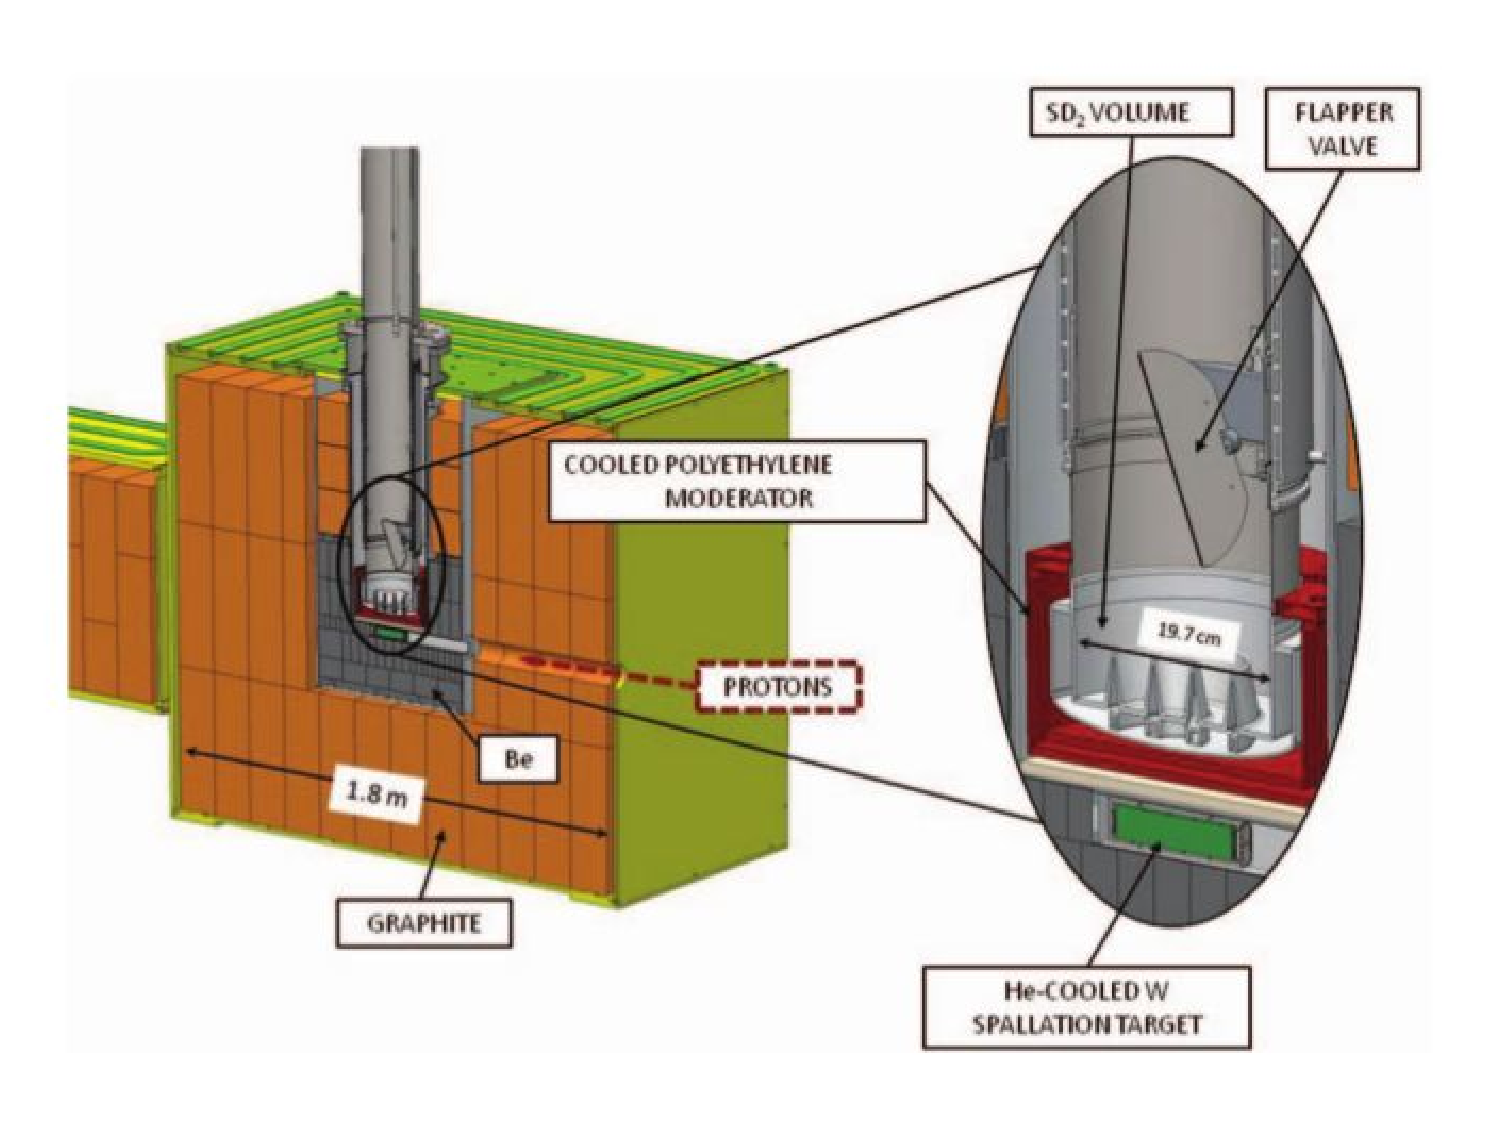
\includegraphics[scale=0.48]{2-UCNAExperiment/source_figure.pdf} 
  \caption{UCN source schematic. Inlay is a zoom in on the
    $\mathrm{SD}_2$ cell \cite{saunders2013performance}.}
  \label{fig:sourceFig}
\end{figure}

A schematic to assist in the understanding of the source at the time of data-taking
for this analysis is found in Figure
\ref{fig:sourceFig}. The process begins with delivery of protons from the 800~MeV proton
accelerator operated in pulsed mode, with pulses repeated at a rate of 0.2~Hz and a typical
integrated proton current on target of $5-10~\mu$A.
The protons strike a helium-cooled tungsten target (12~cm long) and produce
spallation neutrons at roughly 20~MeV. The spallation target is surrounded by
a room temperature beryllium reflector to help direct as many neutrons as
possible towards the UCN source. The solid deuterium ($\mathrm{SD}_2$) UCN source
is located directly above the tungsten target, housed in a liquid helium
cooled cryostat. Prior to entering the $\mathrm{SD}_2$ source, neutrons
pass through a 1~cm thick moderator made of polyethylene beads cooled with the boil off gas
from the cooling of the $\mathrm{SD}_2$ source in the cryostat.
UCN are produced using the superthermal interaction of a cold neutron with the $\mathrm{SD}_2$,
which transfers most of the neutron's energy to a phonon in the crystal \cite{golub1991ultra}.
The $\mathrm{SD}_2$ is constantly cooled with liqiud He, thereby contiuously removing
the heat. 

The $\mathrm{SD}_2$ source is a cylinder 19.7~cm in diameter and 5.7~cm tall. There
is a collection of ``fins'', or vertical teeth-like structures, located in
the bottom of the aluminum cryostat to increase the surface area of contact between the
$\mathrm{SD}_2$ and the liquid helium cooled surface. The surface of the cryostat
is coated with beryllium to reflect as many UCN as possible within the UCN source. Above
the $\mathrm{SD}_2$ is a flapper valve which opens to let UCN out of the source and
prevented UCN from re-entering the $\mathrm{SD}_2$ to reduce upscattering and loss of UCN.

Once a UCN passes the flapper, it is guided along a 1~m vertical guide coated with $^{58}\mathrm{Ni}$.
At this point, the UCN enter stainless steel horizontal guides for transportation from
the biological shielding that surrounds the source. The higher 342~neV potential of the
the $^{58}\mathrm{Ni}$ ensures that all neutrons which are capable of being guided by the
stainless steel (189 neV potential) are confined within the entirety of the vertical guide
\cite{saunders2013performance}. Upon looking at Figure \ref{fig:guides}, one sees that
there are two $45\degree$ bends in the stainless steel guides to remove neutrons still
exceeding the UCN regime \cite{plaster2012}.

\begin{figure}[h]
  \centering
  \includegraphics[scale=0.48]{2-UCNAExperiment/experimentalSetup.png} 
  \caption{Schematic of guides and layout of the UCNA experiment \cite{plaster2012}.}
  \label{fig:guides}
\end{figure}

Once the UCN exit the shielding, they are guided along stainless steel guides
through a gate valve which allows for separation of the UCNA apparatus from the UCN
source while the proton beam is on, thus allowing for background measurements in
the spectrometer
during $\beta$-decay running conditions (proton beam operating, but void of UCN).
Beyond the gate valve is a 6~T pre-polarizing magnet (PPM). The purpose of the PPM
is to minimize the loss of UCN during transport through the Zr foil used to separate
the vacuum in the UCN source from the vacuum in the rest of the apparatus. The neutrons
are nominally polarized longitudinally after passing through the PPM's longitudinal field.

Beyond the PPM, the guides switch to electropolished copper (168 neV potential) to
maintain the initial polarization of the neutrons. Just downstream of the PPM
is the ``switcher'' valve. When the valve is open, the downstream guides are connected
to the guides coming from the PPM carrying UCN. Upon closing the switcher valve,
the downstream guides are redirected to a $^3\mathrm{He}$ 
UCN detector \cite{morris2009multi} used in polarimetry measurements.

Upon bypassing the switcher,
the UCN are guided through the 7~T primary polarizing magnet (or AFP magnet). At this point
the guides switch to 100~cm of diamondlike carbon coated quartz guides \cite{mammei2010thin}
for passage through the Adiabatic Fast Passage (AFP) spin flipper \cite{holley2012high}.
The guides then switch back to circular copper guides before coupling to a rectangular
(4~cm width $\times$ 7~cm height) copper guide which transports the neutrons into the 1~T field
inside the Superconducting Spectrometer (SCS).

Prior to the beginning of running in 2011, a shutter was installed between the decay trap and
the guides used to close the decay trap off from the guides. During normal $\beta$-decay
runs, the shutter is open allowing neutrons to flow into (and out of) the decay trap as they are
created in the source. The shutter then closes at the beginning of a depolarization run, which immediately
follows every $\beta$-decay run, to allow for draining of the guides prior to a depolarization
measurement. This will be discussed in more detail later.

\section{Neutron Polarization} \label{sec:polarization}

The neutrons are initially polarized utilizing the $-\vec{\mu}\cdot \vec{B} \approx \pm 60$~neV/T
potential. The UCN pass through the 6~T pre-polarizing magnet and then
through the 7~T primary AFP polarizing magnet. Neutrons with spin
aligned to the field (remember that the magnetic moment of the neutron is negative and so is antialigned
to the spin) see a positive (repulsive) potential of 420~neV from the 7~T magnet, and thus all
UCN in this spin state are reflected. The opposite spin state sees an attractive potential
and is transmitted, thus producing
a completely polarized population of UCN beyond the AFP magnet.
At this point, the neutrons pass through the AFP spin flipper. If the spin flipper is on, the spins
undergo a $\pi$ spin-flip before being loaded into the decay trap, and when off, the spins are
loaded in the same state that was selected by the AFP magnet.

A detailed description of the spin flipper can be found in \cite{holley2012high}. In short, the
flipper works under the premise of nuclear magnetic resonance (NMR) and utilizes a sinusoidally
varying magnetic field ($B_1$) that is transverse to the primary holding field ($B_0\approx 1$~T).
If there is a finite region where the $B_1$ field exists, i.e. it is zero outside this region and only
the $B_0$ holding field exists, it can be shown that as a spin passes through this region
it will undergo a $\pi$ spin-flip if at some point on the interval
the frequency $\omega$ of the rotating field $B_1$ is equal to the
Larmor precession frequency $\omega_{\mathrm{L}}$ of the spin about the holding field $B_0$.
To ensure that $\omega = \omega_L$ at some point
on the neutron's trajectory through this interval,
a gradient is introduced in the holding field $B_0$ while the frequency of
the rotating field is held constant. With proper tuning, the resonance condition is met, and as long
as adiabaticity is maintained, the spin flips direction. The conditions for adiabaticity defined in terms
of pertinent field parameters for this setup can be found in
\cite{holley2012high}. The most recent polarimetry measurements indicate an efficiency $>99.9\%$ \cite{brown2017}.

\begin{figure}[h]
  \centering
  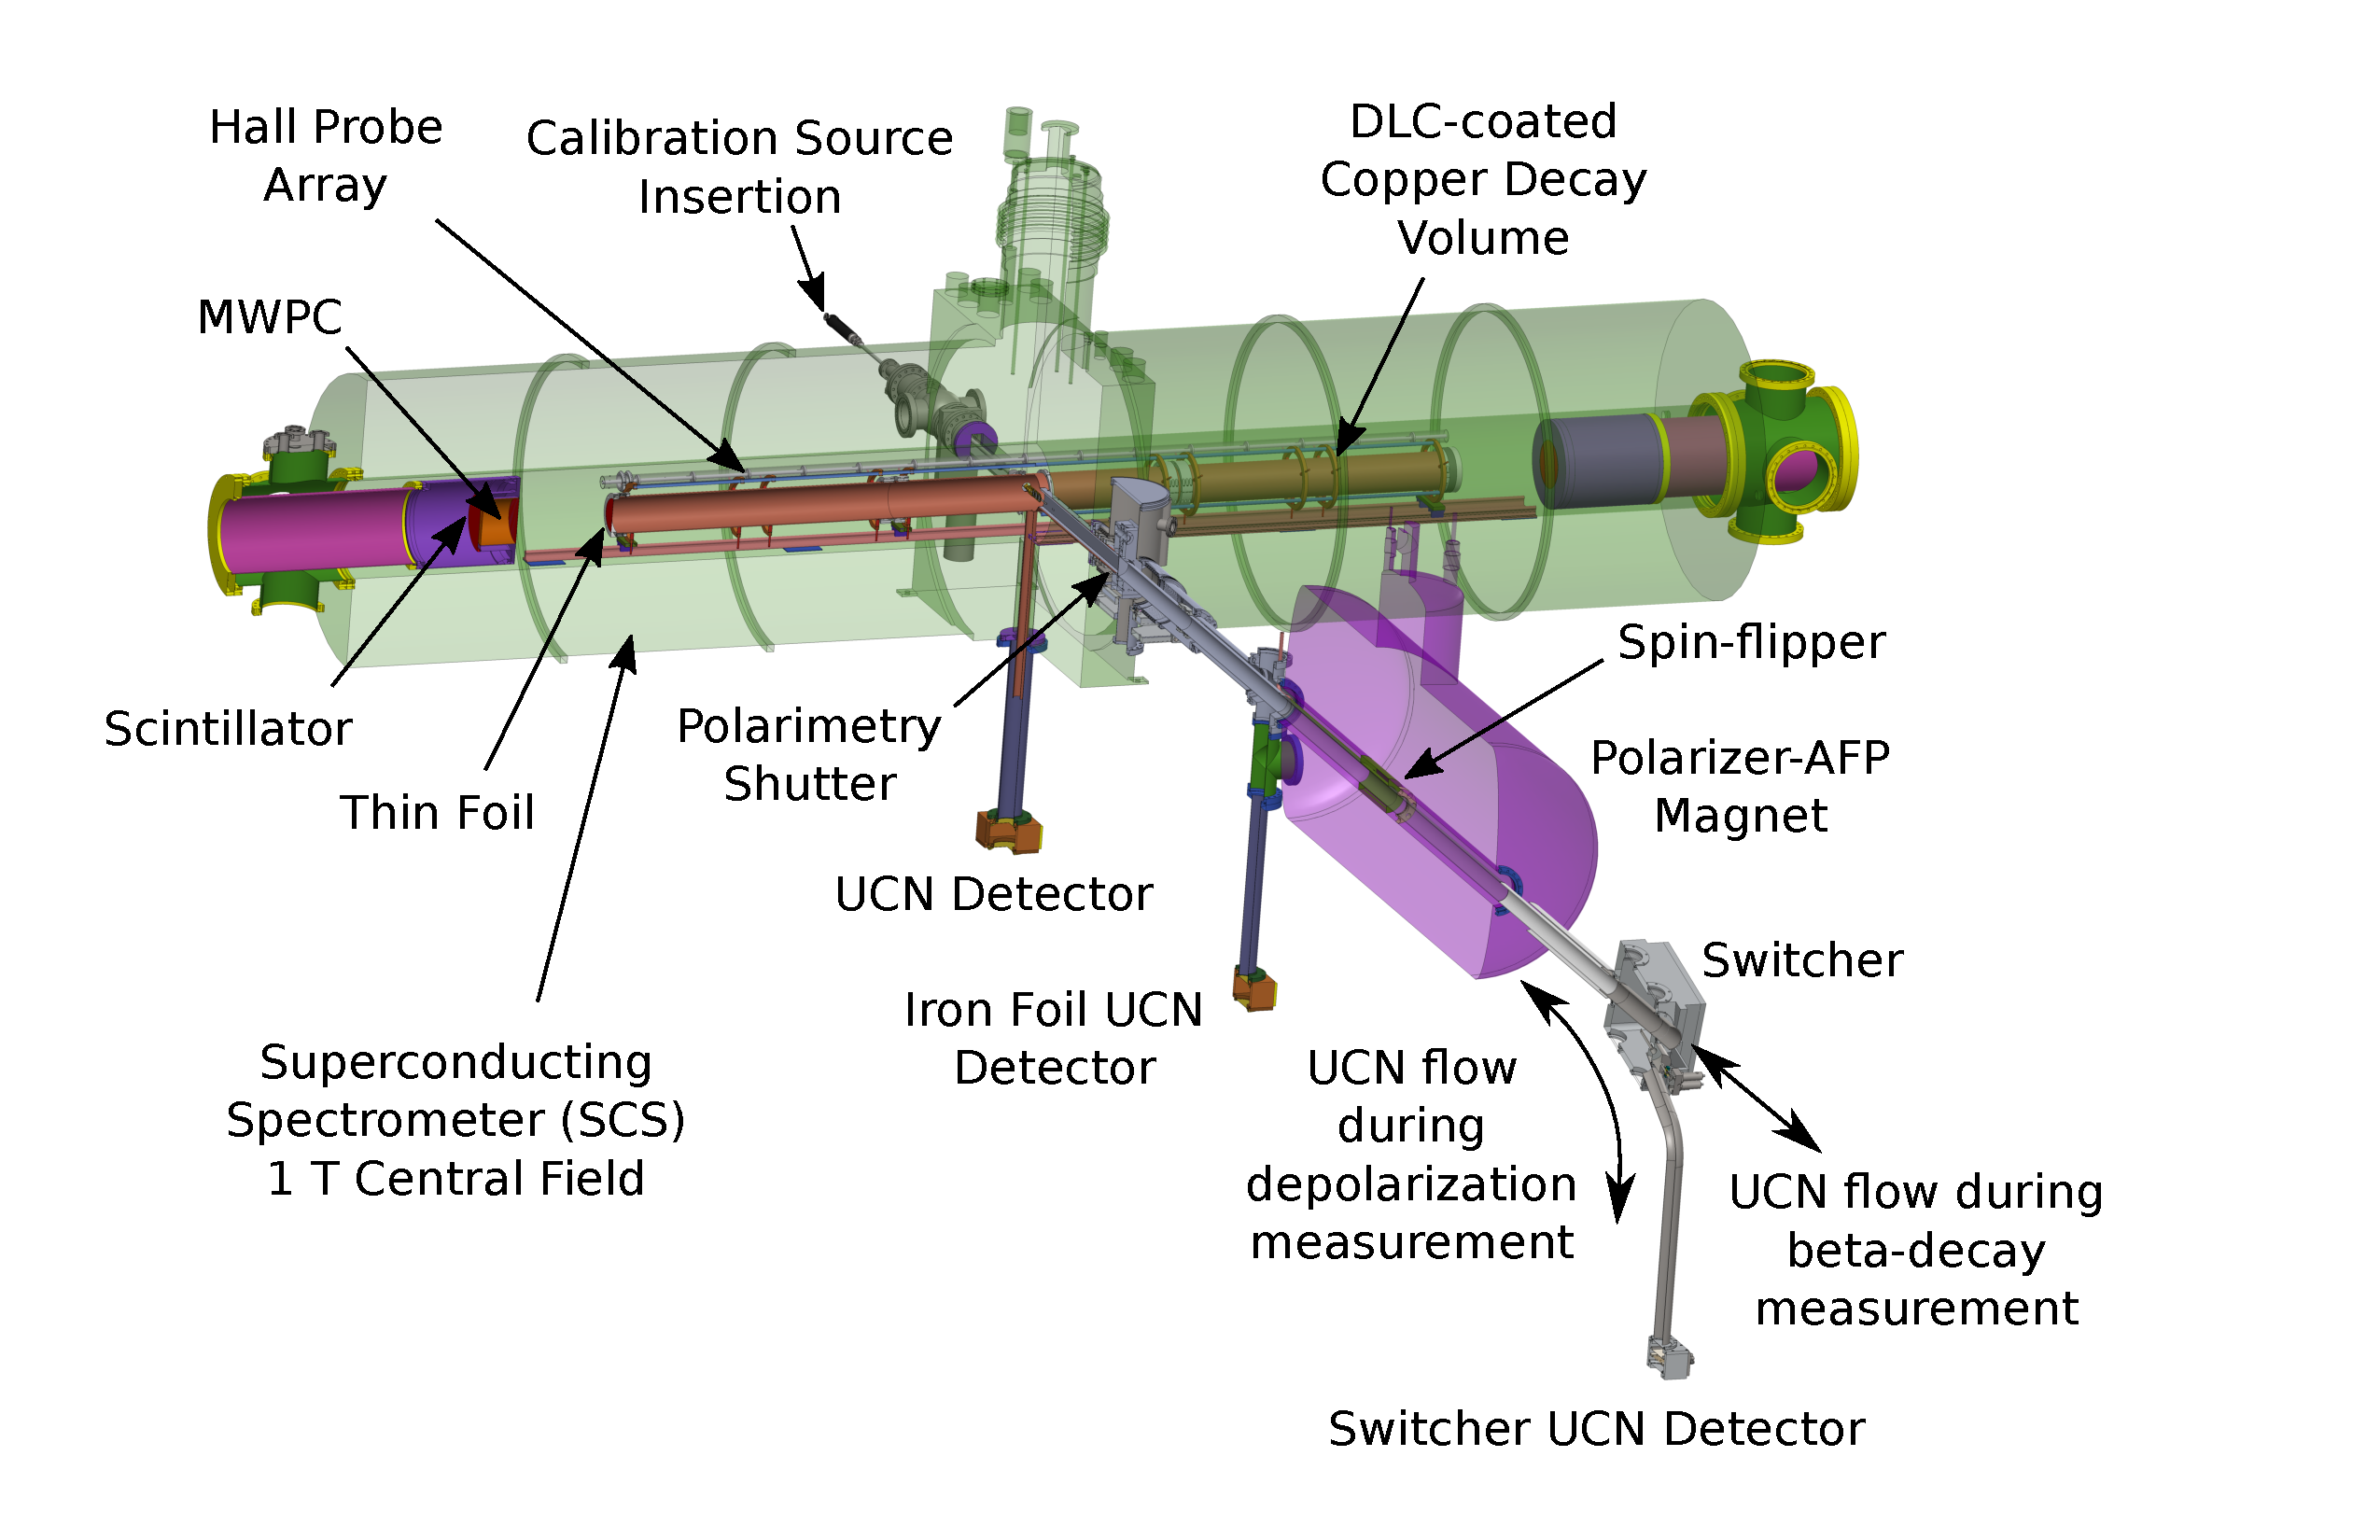
\includegraphics[scale=0.38]{2-UCNAExperiment/UCNAFig.pdf} 
  \caption{Detailed rendering of the experimental area. }
  \label{fig:setup}
\end{figure}

\section{Superconducting Solenoidal Spectrometer}

The spectrometer consists mainly of the superconducting solenoidal magnet designed to produce
the 1~T central field, a decay trap to contain the UCN until they decay, and detector
packages located at each end of the spectrometer to detect decay electrons after they spiral
about the field lines towards either detector. The detectors are referred to as
East and West based on their orientation in the experimental area.
Brief descriptions of the main components follow.

\subsection{Decay Trap}
The decay trap is situated at the center of the spectrometer within the 1~T magnetic
field. The cylindrical 300 cm in length, 12.4 cm in width decay trap is made of electropolished Cu
to confine as many UCN as possible. Typically the vacuum within the decay trap and the guides
upstream to the Zr foil which separated the source vacuum from the experimental apparatus was about
$10^{-5}$~Torr. The density of UCN in the decay trap was monitored using a $^3\mathrm{He}$ UCN detector
directly below a 0.64~cm hole in the decay trap.

One of the main differences between the 2011-2012 and 2012-2013 run periods was the thickness and
material of the decay trap endcaps (sometimes interchangeably referred to as decay trap windows).
In both geometries the endcaps were coated with 150~nm of
Be (potential 252 neV) to aid in reflecting neutrons to confine them, which increases the
UCN density and thus the decay rate. The 2011-2012 endcaps
were 500~nm Mylar on both the East and West detectors, while the 2012-2013 endcaps were made of 6F6F
\cite{hoedl2003} and were 130~nm (East) and 180~nm (West) thick. The change in endcap thickness
is the primary reason for analyzing the two sets of data separately, as this changes the
systematics involving electron backscattering. 

\subsection{Magnetic Field} \label{ssec:MagneticField}

The general requirements for the magnetic field within the decay trap was that it must be aligned with
the axis of the decay trap to define the axis of polarization, strong enough to confine the Larmor
radius of the decay electrons as they spiral toward the detectors, and uniform enough that
electrons will not be reflected.

The necessity for a uniform magnetic field follows from consideration of the flux contained
within the spiral of the electron around the magnetic field lines. From \cite{jackson1999}
we know the flux, $Br_e^2$, is an adiabatic invariant, which means so is $p_\perp^2/B$ where
$p_\perp$ is the transverse momentum of the spiraling electron and $p = \sqrt{p_\perp^2+p_\parallel^2}$.
Given this, there exists a condition for reflection when an electron originates in a field $B_0$
with initial momentum $p_0 = \sqrt{p_{0,\perp}^2+p_{0,\parallel}^2}$
and encounters a field $B_{\mathrm{max}}$,
%
\begin{equation}
  \frac{B_{\mathrm{max}}-B_0}{B_0} > \frac{p^2_{0,\parallel}}{p^2_{0,\perp}}.
  \label{eq:fieldReflection}
\end{equation}
%
A field uniformity of $10^{-4}$ was determined sufficient to remove appreciable effect
on the asymmetry \cite{plaster2008solenoidal}.

The magnet, constructed by American Magnetics, Inc., is a warm-bore 35~cm diameter, 4.5~m
long superconducting solenoid (SCS magnet). Technical details of the magnet can be found in
\cite{plaster2008solenoidal, plaster2012}. An important aspect of the magnetic field not mentioned
previously is the field expansion from 1~T to 0.6~T beyond the decay trap windows but prior to
the wirechambers. This field expansion decreases the pitch angle of the electron,
defined as
$\theta = \cos^{-1}(p_{\parallel}/p)$, as it
enters the detector package as seen from the earlier stated adiabatic invariant $p_\perp^2/B$
coupled with conservation of momentum. Decreasing the pitch angle decreases the probability
of backscattering substantially. One should note here that transverse positions measured using the MWPC
within the field expansion region need to be converted to decay trap coordinates, which is within
the 1~T field region, using $x_{\mathrm{trap}} = \sqrt{0.6} \times x_{\mathrm{MWPC}}$.

\begin{figure}[h]
  \centering
  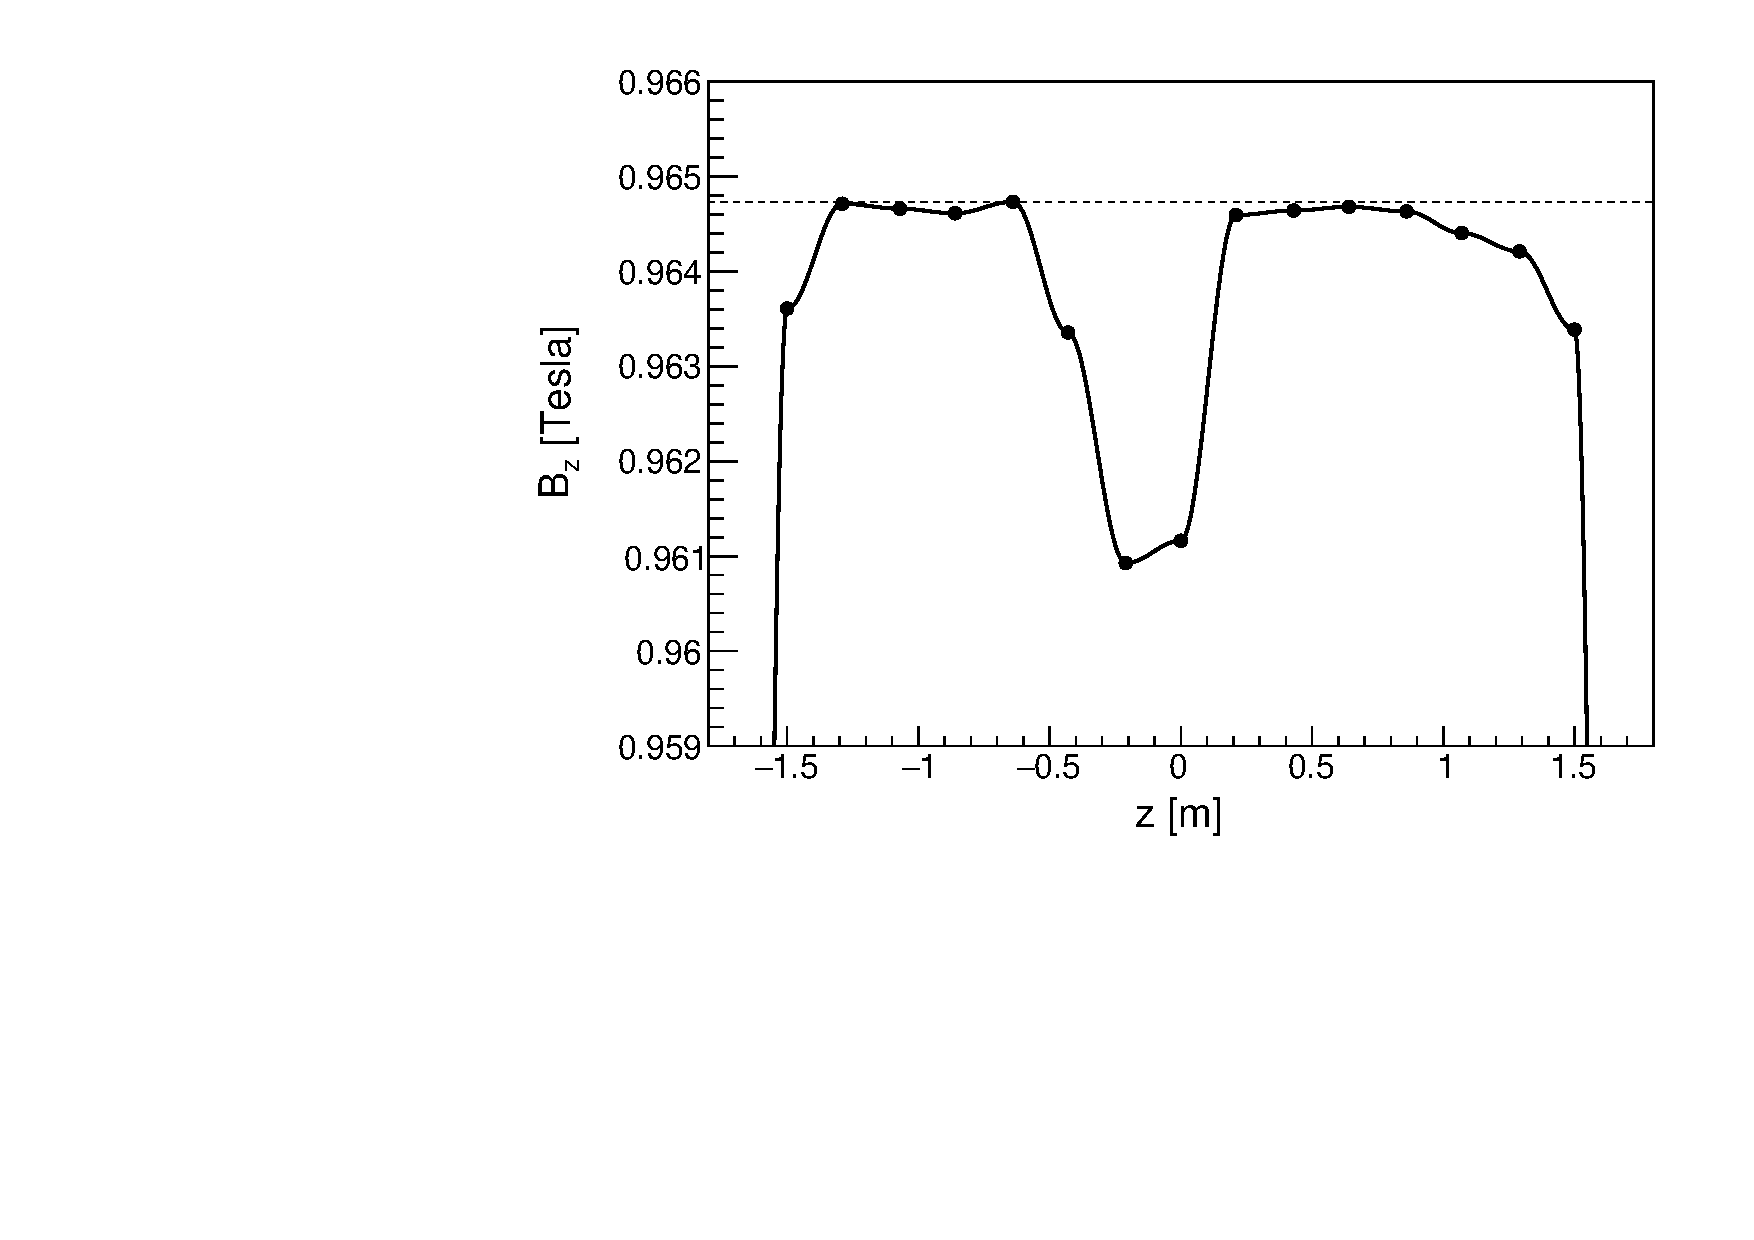
\includegraphics[scale=0.5]{2-UCNAExperiment/magField.pdf} 
  \caption{Typical field profile from 2011-2012 run period. The smooth interpolation between discrete values utilizes a half-wave of a cosine as defined in \ref{sssec:simMagField}.}
  \label{fig:field_profile}
\end{figure}

In 2011-2012 and 2012-2013, the magnetic field was not as uniform as reported in 
\cite{plaster2008solenoidal} due to damage to the shim coil persistence heater switches
caused by multiple magnet quenches \cite{plaster2012}. A typical field profile can be seen
in Figure \ref{fig:field_profile}, where a pronounced dip exists in the center due to the damage
mentioned above. The uniformity outside the dip is at the $10^{-4}$ level, while the dip is
$\sim4\times 10^{-3}$. Electrons
that originate in the dip region can become trapped if the condition in equation
\ref{eq:fieldReflection} is satisfied. The electron then only exits the field dip
upon scattering from the residual gas in the decay trap which randomizes the direction
and energy
of the electron. The effect
on the asymmetry from the field
dip is addressed as a systematic
uncertainty in Section \ref{sssec:MagFieldSyst}.


\subsection{Detector Packages}

\subsubsection{Multiwire Proportional Chamber} \label{sssec:ExpMWPC}

The multiwire proportional chamber (MWPC, or sometimes called the wirechamber throughout this work)
\cite{ito2007,plaster2012} is
utilized to reconstruct the transverse position of the electron events and to reduce the ambient
backgrounds. The MWPC consists of an anode plane in between two cathode planes, with the cathode
planes oriented perpendicular to one another to allow for position reconstruction in both directions
transverse to the axis of the SCS. There are
64 wires in each plane with 2.54~mm spacing between each wire. The spatial extent of the
MWPC is $16.3 \times 16.3\mathrm{~cm}^2$ which maps to
$ (\sqrt{0.6} \times 16.3) \times (\sqrt{0.6} \times 16.3) \mathrm{~cm}^2 = 12.6 \times 12.6\mathrm{~cm}^2$ coverage
within the decay trap (remember the decay trap is within the 1~T field while the detectors
are in the field expansion region with field of 0.6~T), thus the wirechamber covers the full
decay trap cross-sectional area. The anode wires are $10\mathrm{~\mu{m}}$ in diameter while the cathode
wires are $78.2\mathrm{~\mu{m}}$ in diameter, with the diameter of the cathode wires slightly
larger than in previous run periods ($50\mathrm{~\mu{m}}$).

\begin{figure}[h]
  \centering
  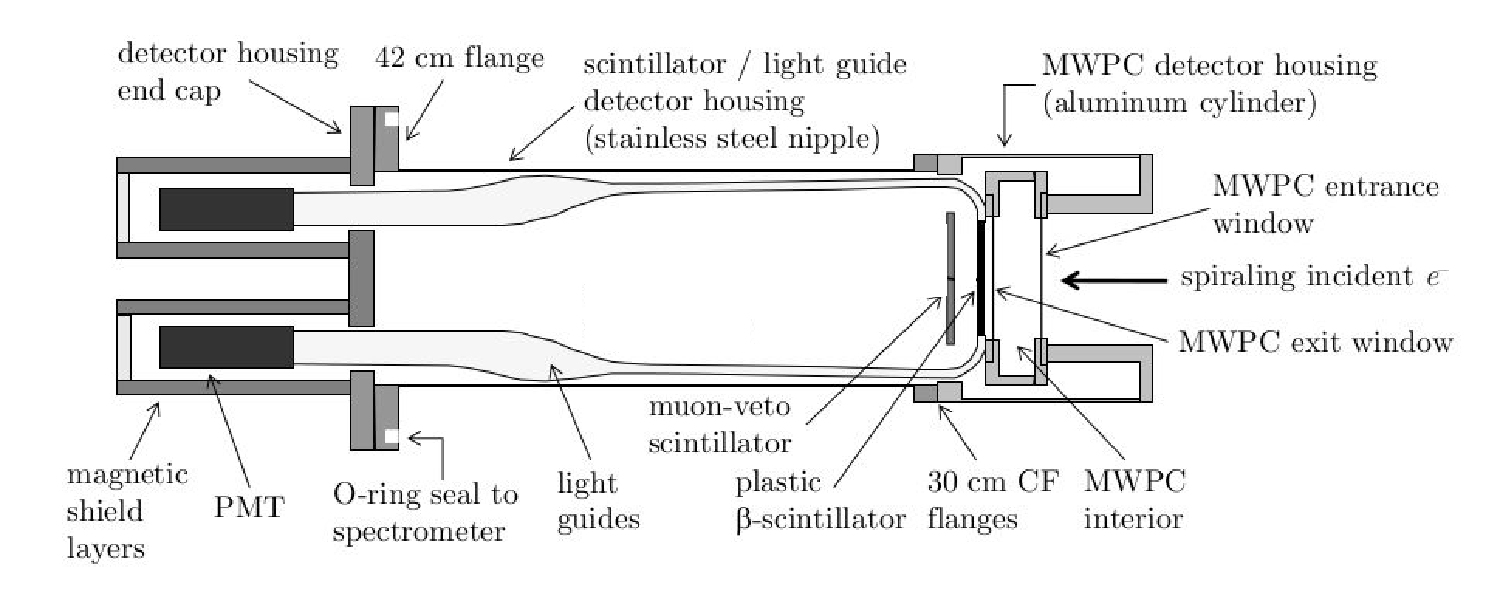
\includegraphics[scale=0.6]{2-UCNAExperiment/detector_setup.pdf} 
  \caption{Schematic of the detector packages \cite{plaster2012}.}
  \label{fig:detectors}
\end{figure}

Charged particles passing the MWPC ionize the gas, and the $\sim2700$~V bias between the anode and
cathode plains causes the ions and electrons to drift towards the cathode and anode respectively,
inducing a signal in the wires proportional to the ionization created by the traversing charged particle.
The anode wires are read out as a summed signal, with all 64 wire signals summed corresponding to
a single ADC channel. This signal is typically used in relating the total signal in the MWPC
to an energy deposited within the wirechamber. The cathode wires are read out in groups of four
consecutive wires, so there are 16 ADC channels for each wirechamber cathode plane. These 16
``wires'' (as we will call them from now on) are used for position reconstruction. Either
signal can be effectively used for the MWPC software trigger.

The fill
gas chosen for the MWPC should be low Z (low atomic number) to minimize the backscattering from heavy nuclei
($d\sigma/d\Omega \propto Z_{\mathrm{target}}^2$),
but also electron dense to increase the ionization efficiency. Thus complex large molecules
made up of low Z nuclei are good candidates.
The MWPC during running was primarily filled with neopentane ($\mathrm{C}_5\mathrm{H}_{12}$) gas at a pressure of
100~Torr, chosen to ensure enough gain for electrons within the $\beta$-decay spectrum. For a
short time period in 2012-2013, the neopentane ran out and isobutane ($\mathrm{C}_5\mathrm{H}_{10}$)
was used instead. Separate simulations were used for the isobutane runs, but no appreciable
difference was noticed.

The windows on the wirechamber are made as thin as possible so as to reduce backscattering, but still
retain their integrity under the 100~Torr pressure difference between the SCS and the wirechamber. Events that
scatter off of the entrance window are particularly troublesome as they become missed backscattering events.
The chosen front window material is $6\mathrm{~\mu{m}}$ of aluminized Mylar reinforced with Kevlar strings
placed at 5~mm increments, and the exit window is also $6\mathrm{~\mu{m}}$ of aluminized Mylar \cite{mpmThesis}. 

The importance of the MWPC should not be understated. First of all, the position reconstruction allows for the
definition of a fiducial volume within the decay trap so that we can cut out events which may have interacted
with the decay trap walls. Such interactions change the energy/direction of the electron, so simply removing them
reduces the systematic correction necessary. Secondly, the scintillator light transport to the PMTs is position
dependent, so the position of each event is needed to properly assign a reconstructed initial energy to
each electron event. The MWPC is also vital in identifying backscattering events by looking at the energy
deposited within the wirechamber, i.e. an event that backscatters off of the dead layer of the scintillator
will deposit energy in the MWPC above some software cut and can be identified. And last of all,
the wirechamber is highly insensitive to gamma rays, thus, by including a coincidence trigger between the wirechamber
and the scintillator, the majority of the gamma background is removed. The insensitivity is due to
the low Z, low density gas making the probability of compton
scattering small. Also, the $\sim$few~MeV gamma background along with the low Z gas makes pair production
unlikely as well.

\subsubsection{Scintillator}

A 15~cm diameter, 3.5~mm thick plastic scintillator \cite{plaster2012}
from Eljen Technology (EJ-204) is located beyond the
MWPC. The maximum stopping distance for an endpoint (782~keV) electron is 3.1~mm, so the
scintillator is capable of reconstructing the entire energy spectrum. To transport the
scintillation light out of the 0.6~T field to the photomultuplier tubes (PMT),
located about 1~m from the scintillator where the field is $\sim0.03$~T,
twelve light guides are coupled to the edge of the scintillator using optical grease.
From there, the twelve guides are adiabatically merged into four
larger guides which are attached to four Hamamatsu R7725 PMTs with custom bases \cite{hickerson2013}.
The light guides are merged and coupled to the PMTs in such a way that each PMT effectively
covers one quadrant of the scintillator.
A hardware two-fold trigger, defined as two or more PMTs above discriminator threshold, is required for a
global trigger to be issued from the PMTs.

\begin{figure}[h]
  \centering
  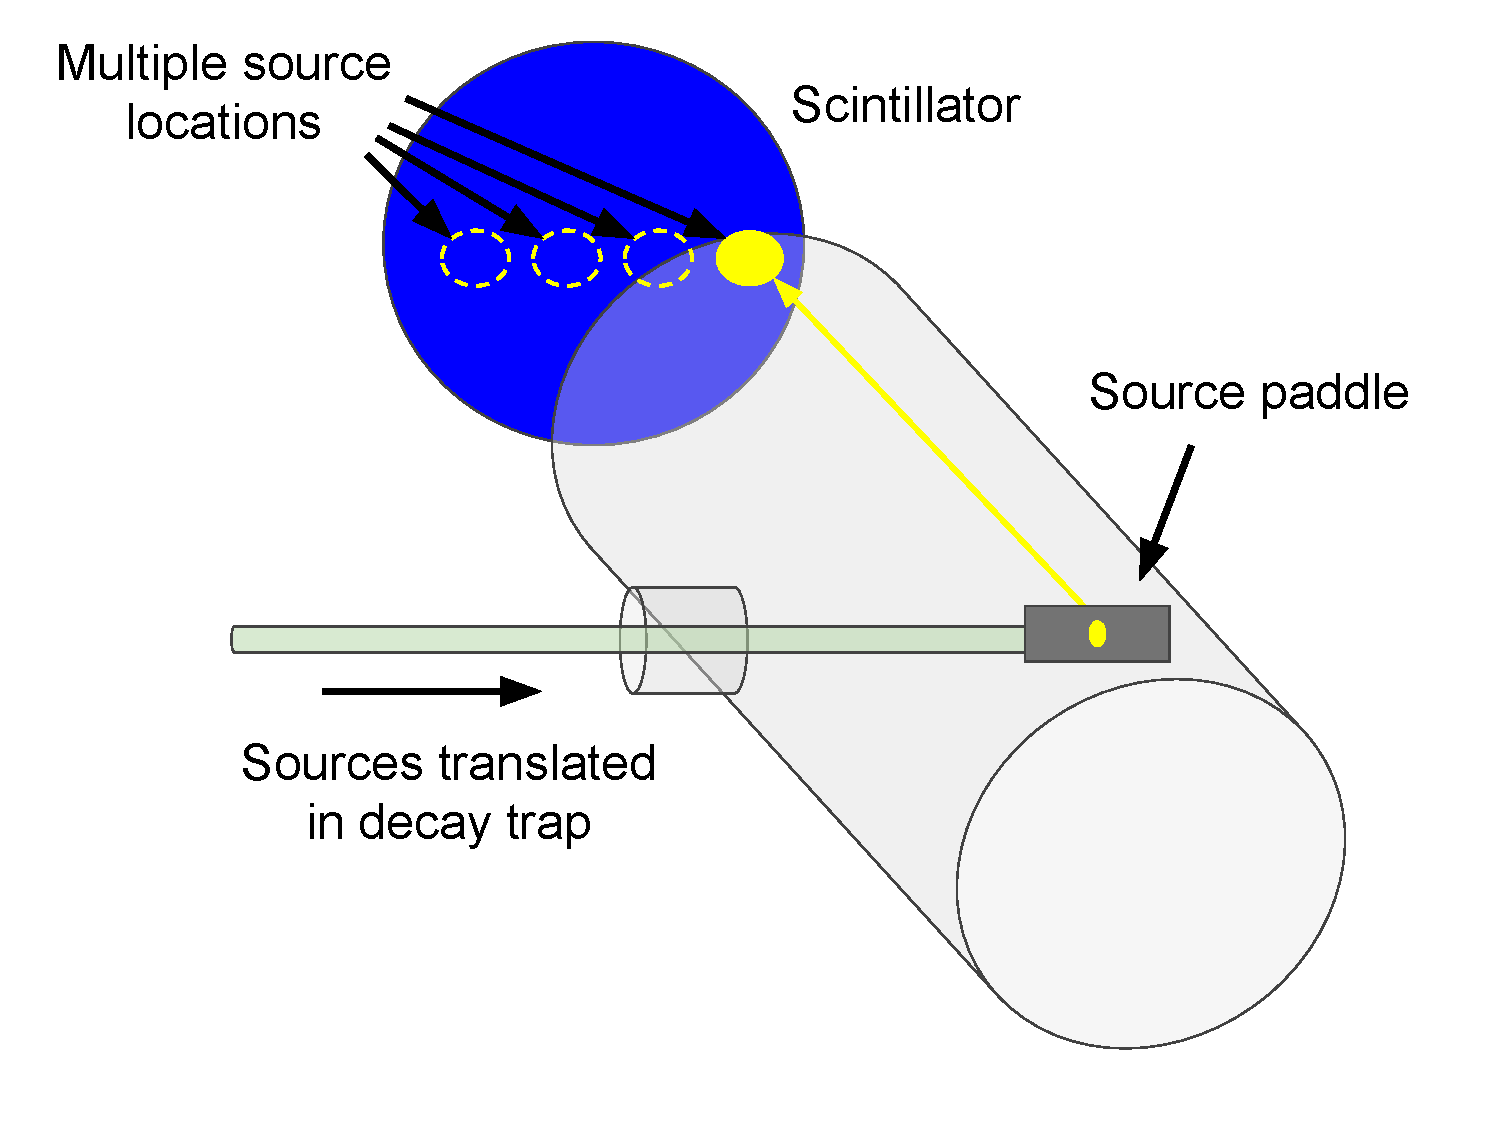
\includegraphics[scale=0.5]{2-UCNAExperiment/calProcess.pdf}
  \caption{Schematic showing the mechanics of the scintillator calibration. The sources
    are located on a source paddle, which is inserted into the decay trap while under
    vacuum. The sources are then translated across the face of the detector, and a
    calibration run is completed at each stationary point. There are generally far more
    than four positions sampled, but for demonstrations sake only four points are
    included in the figure.}
  \label{fig:sourceTranslate}
\end{figure}

\subsubsection{Scintillator Energy Calibration} \label{sssec:scintEnCal}

The scintillator energy calibration utilized the conversion electron lines from
(with dominant K-shell energies listed) $^{137}\mathrm{Ce}$
(130.3 keV), $^{113}\mathrm{Sn}$ (363.8 keV), and $^{207}\mathrm{Bi}$ (481.7~keV and 975.7 keV)
sources. As depicted in Figure \ref{fig:sourceTranslate},
these sources are placed on a source paddle and inserted into the side of the
decay trap while under vacuum, and then they are translated across the horizontal axis of the decay
trap. This method probes the position dependence of the scintillator, but only along one axis and
at discrete points (the sources are manually translated in between runs, thus the discrete source locations
are a result of the required time and effort of the experimenter on shift).
The full light transport position response of the scintillator is captured using another method as will be
described later. Also detailed later in Section \ref{ssec:BiGain}, the gain of the PMTs is monitored
and drifts corrected 
on a run-by-run basis using a $^{207}\mathrm{Bi}$ ``pulser'' system \cite{morris1976stable}.

\subsubsection{Muon Veto System}

Cosmic ray muons can create a scintillator two-fold trigger and pass the software trigger in
the MWPC, so they trigger the same components of the detector as a $\beta$-decay electron. By identifying
the muons through means other than the scintillator or wirechamber, the muon events
can be vetoed during analysis. The first veto mechanism used
is an argon/ethane sealed drift tube system \cite{rios2011sealed}. The drift tube veto sits
above the spectrometer, partially wrapped around the sides. Muons ionize the gas inside the
tube, and thus by checking for a coincidence in the drift tube, one can remove muons
and events from secondary electrons created by the muons. The second method of monitoring
muon events is the use of scintillators placed directly behind the primary
electron scintillator as seen in Figure \ref{fig:detectors}. The primary detector
stops all $\beta$-decay electrons, so a coincident signal in the ``backing veto''
indicates that a muon or some other event passed through the detector package.

\section{Data Signals and Trigger Logic}

Details regarding the data acquisition system can be found in \cite{plaster2012,mpmThesis},
so the electronics will be left out of this discussion. Instead, what is more important for
understanding the work contained within this thesis is the primary logic used to
determine an electron event, and the terminology used when discussing different signals.

The two primary types of signals mentioned are ADC and TDC signals.
An ADC signal is a number related to a voltage output by a detector component, and this
signal may either be an integrated signal or a peak sensing signal. Either way, it is related
to the ``strength'' of the signal as seen by the detector component, which is the energy deposited
in most cases. An example of an ADC signal can be seen in Figure \ref{fig:ADCsig}, where we show the
detector output over one run for a single PMT during a $\beta$-decay run.
The second signal used is a TDC signal, which for our purposes is
just a timing signal to indicate when a detector component triggered, or if it triggered at all.
An example TDC signal can be
seen in Figure \ref{fig:TDCsig}.

\begin{figure}
  \centering
  \subfloat[Raw ADC signal for a single PMT]{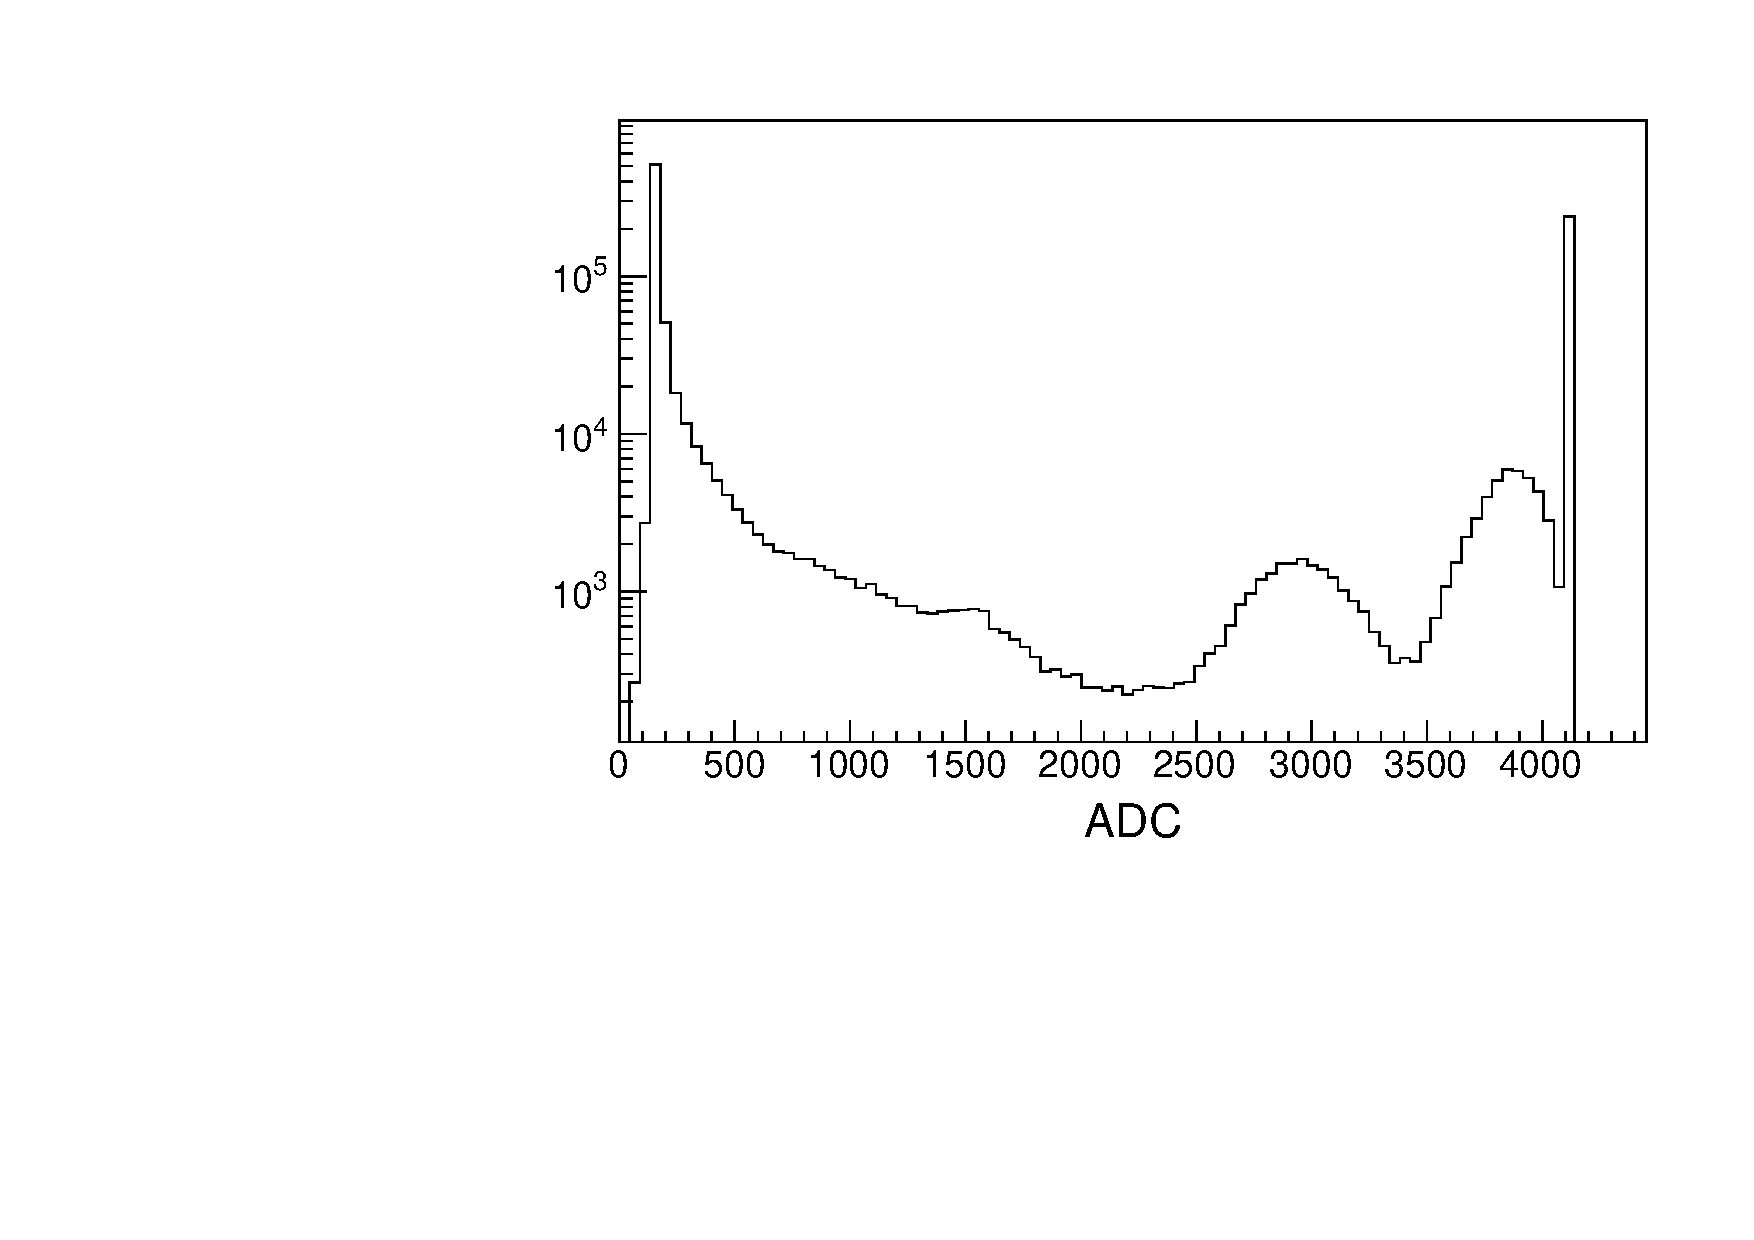
\includegraphics[page=1,scale=0.38]{2-UCNAExperiment/rawADCsignal17126.pdf}}
  \subfloat[Raw ADC signal for a single PMT with two-fold scintillator trigger applied]{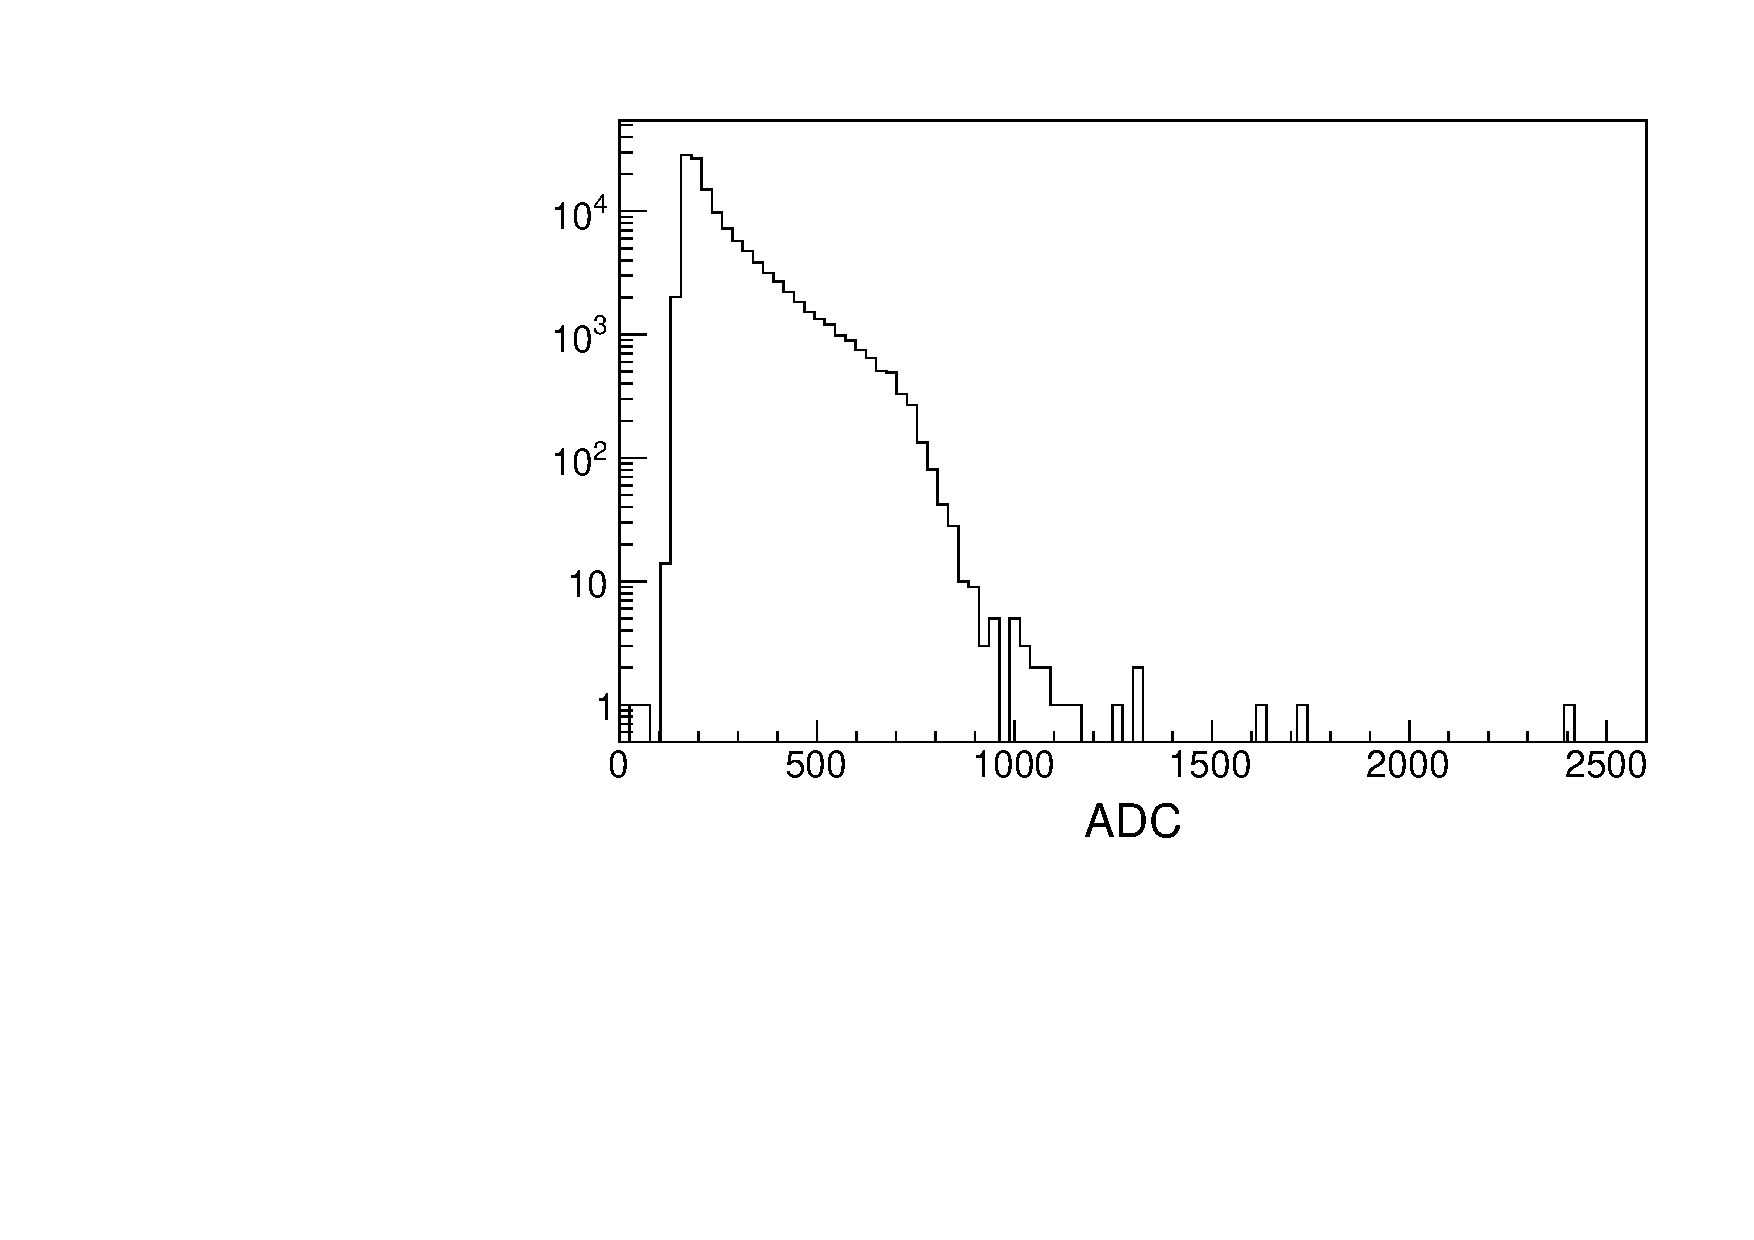
\includegraphics[page=1,scale=0.38]{2-UCNAExperiment/rawADCsignal17126_betaEast.pdf}}
  \caption{Comparison of the raw ADC signal from a single PMT for any global trigger in panel a.) and upon requiring a two-fold PMT trigger
    on the side of the PMT of interest in panel b.). This type of cut is part of the electron trigger along with a coincidence with the wirechamber.}
  \label{fig:ADCsig}
\end{figure}

\begin{figure}
  \centering
  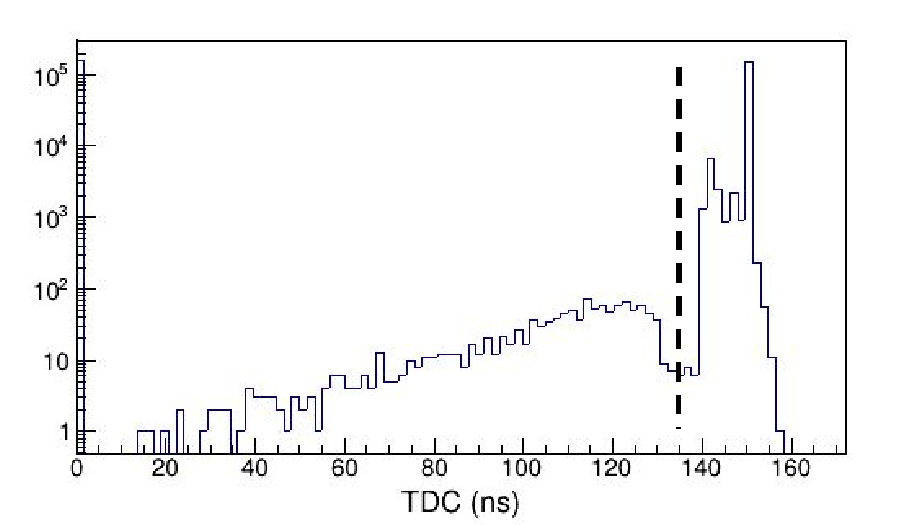
\includegraphics[page=1,scale=0.60]{2-UCNAExperiment/TDCSignal.pdf}
  \caption{Example TDC signal (converted to nanoseconds) from a $\beta$-decay run for a single
    detector.
    Note that the horizontal axis is technically the time elapsed since a trigger occurred,
    so a longer time indicates an earlier
    trigger. The dashed line
    indicates the cut used to separate a self-trigger (right of the dashed line) from a backscattering trigger
    (left of the dashed line).  The events at $t=0$ are events which did not create a self-trigger.}
  \label{fig:TDCsig}
\end{figure}


Several types of signals can generate a global trigger, where the data acquisition system (DAQ)
reads all possible inputs. These include:
%
\begin{itemize}
\item UCN monitor $-$ used to monitor the UCN production at various
  stages along the experimental apparatus.
\item $^{207}\mathrm{Bi}$ pulser event $-$ This is a high threshold, single PMT trigger, so if one PMT
  has a trigger above a pre-set high threshold, but no other PMT has any trigger, this indicates the
  pulser created the trigger at the PMT and not the scintillator. This will be addressed more in the
  next chapter.
\item LED pulser $-$ An LED system was in place to assist in correcting any non-linearity in the
  PMT response. The light output of the LED is adjustable, and so by varying the light output of
  the LED to the PMTs, the linearity could have been monitored.
  This was not utilized in this analysis, but still results in a global trigger.
\item Two-fold PMT trigger $-$ at least two of the four PMTs on one side must have signal above a pre-set
  threshold. This two-fold trigger indicates a particle deposited energy in the scintillator,
  distinguishing it from noise in a single PMT, a $^{207}\mathrm{Bi}$ pulser event, or an LED event.
\end{itemize}


%UCN monitor detectors with a signal over threshold,
%a single PMT high energy trigger which indicates a $^{207}\mathrm{Bi}$ gain monitor trigger,
%or a two-fold PMT trigger.

The two-fold PMT trigger is of most importance for the analysis that follows, as this indicates
that there was sufficient energy deposition in the scintillator to be an electron event.
The hardware trigger does not
discriminate between what type of event may have created the trigger though, so any particle
that can deposit energy in the scintillator could have been the culprit. To remedy this, we rely
on methods already highlighted in above sections. By applying a software trigger to
the wirechamber, we can require that any event that created a two-fold scintillator trigger
in detector 1 must also pass the software trigger in MWPC 1. This almost entirely removes the
gamma background, as the wirechamber is virtually transparent to a gamma.
Then by checking for muon veto signals above some software threshold we eliminate
cosmic ray muon backgrounds, leaving primarily electron events. Of course
some background events make it into the analysis, but these are accounted for
via background subtraction as will be discussed.

Along with ADC signals proportional to energy deposition, all PMTs also report hardware trigger
timing information (TDC signal). Along with the individual TDC signals, a two-fold TDC signal for
each detector is recorded when there is a global trigger.
For backscattering events which trigger both detectors, we use the two-fold TDC signals
to determine the primary side, or the initial direction of the electron. This can be seen in
Figure \ref{fig:TDCsig}. The dashed line indicates the position of a cut to separate a primary trigger
from a backscattering trigger. An acceptable event either has a single primary trigger or a primary
trigger on one side and a backscattering trigger on the other side. 



%%%%%%%%%%%%%%%%%%%%%%%%%%%%%%%%%%%%%%%%%%%%%%%%%%%%%%%%%%%%%%%%%%%%%%%%%%%%%%


\section{Data Taking Structure}

The data is broken into three types of run periods, namely $\beta$-decay data, source calibration, and
Xe position mappping. The latter two determine the parameters of the energy calibration to be
applied to the data runs. The source calibration and Xe position mapping run periods
occur periodically throughout each data set and are applied to surrounding $\beta$-decay runs. This
creates different subsets of data to which each calibration is applied, as will be illustrated
throughout the rest of this dissertation. Here we simply highlight the structure of the
$\beta$-decay runs, and one should take note that the source calibrations and Xe position map periods
are spaced throughout.

\subsection{$\beta$-Decay Run Structure}
We utilize what we call an octet run structure, where each octet contains a total of twenty-four
runs, eight of which are $\beta$-decay data runs, eight of which are background runs, and eight
of which are depolarization runs. The octet is further split into two halves, A and B, which define
the order of the runs within them as seen in Table \ref{tab:octetStructure}. Whether the A structure
or the B structure comes first within an octet is determined randomly. There are four $\beta$-decay
runs of each spin-state (aligned and anti-aligned to the magnetic field in the spectrometer), and their
accompanying background runs allow for background subtraction. 
The utility of using the octet run structure lies in the fact that, upon proper combination of background
subtracted rates during analysis, any linear drifts in the background rates cancel to all orders \cite{plaster2012}.

%By the same

\begin{table}[h]
  \caption{Octet structure, where $\pm$ indicates spin flipper on/off,
    B refers to background run, D refers to depolarization run, and $\beta$
    refers to $\beta$-decay runs.} 
  \centering
  \begin{tabular}{llllllllllll}
    \hline \hline \\ [-1.75ex]
    A1 & A2 & A3 & A4 & A5 & A6 & A7 & A8 & A9 & A10 & A11 & A12 \\ 
    B$^-$ & $\beta^-$ & D$^-$ & B$^+$ & $\beta^+$ & D$^+$ & $\beta^+$ & D$^+$ & B$^+$ & $\beta^-$ & D$^-$ & B$^-$ \\
    \hline \\ [-1.75ex]
    B1 & B2 & B3 & B4 & B5 & B6 & B7 & B8 & B9 & B10 & B11 & B12 \\
    B$^+$ & $\beta^+$ & D$^+$ & B$^-$ & $\beta^-$ & D$^-$ & $\beta^-$ & D$^-$ & B$^-$ & $\beta^+$ & D$^+$ & B$^+$ \\
    \hline
  \end{tabular}
  \label{tab:octetStructure}
\end{table}





\section{Backscattering} \label{sec:backscattering}
Before moving forward, it is important to formally introduce the different
backscattering events, as they will be referenced often. A backscattering
event is an electron event initially emitted towards one detector, but that
is scattered through a large enough angle that its momentum is reversed and
it travels to the opposite detector. Some of these events are backscattered
by a detector component and can therefore be identified as having backscattered
due to energy deposition on both sides of the spectrometer,
while others backscatter without depositing enough energy (or backscatter prior
to reaching the detector) and therefore become what we call ``missed''
backscattering events. Missed backscattering events are problematic as they
are assigned the wrong intitial direction and therefore systematically effect
the asymmetry.

\begin{figure}[h]
\centering
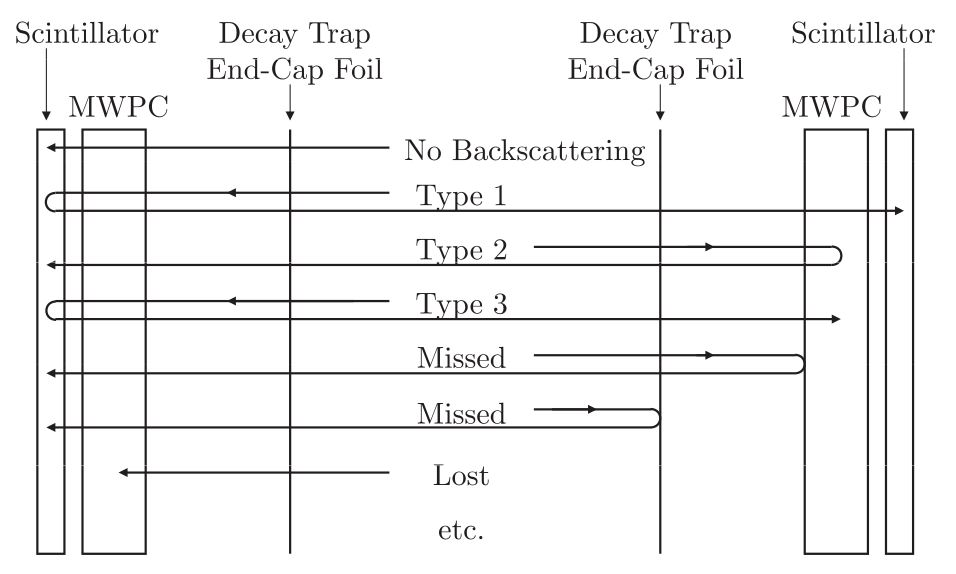
\includegraphics[scale=.4]{3-UCNAAnalysis/backscatterSchematic.png}
\caption{Schematic of different event types and the trigger logic involved with identifying
  each type \cite{plaster2012}.}
\label{fig:backscatterSchematic}
\end{figure}

Based on which detector components trigger, we classify events
into those that do not observably backscatter
(Type 0) and those that do backscatter (Types 1, 2, and 3) \cite{plaster2012}.
A schematic of the different event types can be seen in Figure \ref{fig:backscatterSchematic}.
Type 0 events, while not explicitly listed on the schematic, are a combination of the ``no
backscattering'' and ``missed'' events. They
trigger one scintillator and one MWPC on the same side. Type 1 events are
backscattering events that trigger 
both scintillators and both MWPCs. For such events, we assign the initial
direction to the triggering detector for Type 0 and to the earlier triggering detector
for Type 1. Type 2/3 events comprise a class of events that backscatter and trigger both
MWPCs, but only trigger a single scintillator. Since the MWPCs do not contain any
timing information,
the initial direction of such events can
not be determined from trigger logic alone, as can be demonstrated by considering two events
which look identical under trigger logic.
For example, let ``Event 1'' denote an event that initially backscatters off
of MWPC 1 before reaching scintillator 1
and then traverses the length of the decay
trap to trigger both MWPC 2 and scintillator 2 on the opposite side.
Then, suppose ``Event 2'' denotes another event emitted
in the opposite direction to event 1. Suppose this event
triggers MWPC 2 and scintillator 2
only to backscatter from the scintillator and travel to MWPC 1 and stop short
of scintillator 1. Both events trigger MWPC 1 and 2 and scintillator 2,
but the two events had opposite initial directions, so inclusion of the
two events without further knowledge of their initial direction creates
a dilution to the asymmetry.

An important distinction, however, does exist between Type 2 and Type 3 events:
Type 2 events only pass through the MWPC on the
triggering scintillator side once, whereas Type 3 events scatter from
the scintillator, and therefore pass through the MWPC twice on
the triggering side. We can consequently apply a cut on the energy deposited in
the MWPC on the triggering side to statistically assign
Type 2/3 events to the correct side.
This drastically reduces
Monte Carlo corrections for such backscattering events as simulation indicates we
properly identify $>80\%$ of all Type 2/3 events across all energies using this
technique, a marked
improvement over the roughly $50\%$ misidentification rate without separation.









\copyrightnotice

% Chapter 3
\chapter{UCNA Analysis}
\label{ch:UCNA_Analysis}
%%%%%%%%%%%%%%%%%%%%%%%%%%%%%%%%%%%%%%%%%%%%%%%%%%%%%%%%%%%%%%%%%%%%%%%%%%%%%%%
%%%%%%%%%%%%%%%%%%%%%%%%%%%%%%%%%%%%%%%%%%%%%%%%%%%%%%%%%%%%%%%%%%%%%%%%%%%%%%%
%%%%%%%%%%%%%%%%%%%%%%%%%%%%%%%%%%%%%%%%%%%%%%%%%%%%%%%%%%%%%%%%%%%%%%%%%%%%%%%

\iffalse
Designing an experiment and collecting the right data are non-trivial alone,
but interpreting the results lends itself to a whole new train of thought.
The rest of this thesis is spent describing the details of such an
analysis, with this chapter summarizing important aspects,
such as terminology to be used later and the
model used to characterize our detector response.
\fi

This chapter is dedicated to introducing important aspects of the analysis that
is not strictly tied to calibrations and asymmetry extraction, but rather
data collection and processing to turn raw detector signals into values that
can be calibrated and analyzed. 





%--------------------------------------------------------------

\section{Outline of Analysis Steps} \label{sec:outline}

To preface the rest of this chapter, we begin by highlighting
the general process of the analysis beginning with a raw detector
ADC value from each PMT and finishing with an asymmetry.
Below are the general steps for processing the data:

\begin{itemize}
\item Determine pedestals for each PMT and subtract the pedestal from each data event.
\item Measure the gain of each PMT and divide the drifts out of the signal.
\item Apply a PMT-by-PMT calibration to determine the expected position dependent
  energy deposited in the scintillator
  for each event.
\item Correct for the position dependent response of each PMT
  to return a visible energy as seen by each PMT, $E_{\mathrm{vis},i}$.
\item Combine the four PMT energies into a single deposited energy, $E_{\mathrm{vis}}$.
\item Convert this combined estimate of the energy deposition to a final
  reconstructed energy, $E_{\mathrm{recon}}$, to use in analysis.
\item Calculate an asymmetry and apply all systematic corrections.
\end{itemize}

Simulations of the experimental apparatus and particle transport is also intertwined
in the analysis. By simulating the underlying physical processes, we gain an understanding
as to what the signals in our detector indicate regarding the initial event. The simulations
consist of particle tracking and the summation of energy losses throughout
the spectrometer, and also a Detector Response Model to transform the simulation variables
into detector-like signals. This process will be addressed in Section \ref{sec:DetectorResponseModel}.

It is important to point out early on the difference between $E_{\mathrm{vis}}$ and
$E_{\mathrm{recon}}$. The deposited or visible energy, $E_{\mathrm{vis}}$, is an estimate of the energy
physically deposited in the
scintillator by a particle, while the reconstructed energy, $E_{\mathrm{recon}}$, is an estimate of
the true initial energy of an event. The two are different due to the electron losing energy
as it traverses through the windows of the decay trap, the windows of the MWPC,
the MWPC itself, and the dead layer of the scintillator. Of course the analysis could be
done in terms of $E_{\mathrm{vis}}$, but it is more convenient to express the results
in terms of the true electron energy spectrum, and also the energy dependent theory modifications
are in terms of the true initial energy of the $\beta$-decay electrons.

The majority of the analysis described throughout this thesis was completed using
the ROOT Data Analysis Framework \cite{brun1997root}. A special thanks goes out to
the Nuclear Physics community as a whole, who have collectively built an indispensible
web of documentation regarding any and all things ROOT. Without the ROOT documentation
and user community, much of this analysis would have been painstakingly more difficult.




\section{Time-dependent Detector Corrections}

Obviously the system is not immune to drifts in signals due to variations
in time. There are many sources of such drifts, ranging from simple
electronic noise to changes in temperature. We deal with time-dependent
effects using pedestal subtraction, gain correction, and constant monitoring
of backgrounds.

\subsection{Pedestal Subtraction} \label{ssec:pedSubtraction}
The pedestal is a measure of the underlying detector signal, or baseline, 
upon which all other data signals lie. In terms of PMT signals, you can imagine 
the pedestal as a non-zero ADC value corresponding to zero input, or an offset.
You might say that the experiment can be run without caring about an offset
because the calibration will take this into account, which would be the case 
if the pedestals were constant or if we calibrated each run against itself, but 
neither is the case. We use a collection of consecutive runs to form our 
calibration sets, and these sets then calibrate data which is often taken hours,
or even days, earlier or later. Thus time-dependent pedestals can be worrisome, and care
must be taken to determine the pedestals and subtract them from data signals.

To determine a pedestal, events must be chosen where there was a global trigger, but
the PMT of interest does not trigger and preferably there is no signal
whatsoever in the scintillator on that side. Obvious choices for these events are
UCN monitor triggers, opposite side two-fold PMT triggers, and high-threshold $^{207}\mathrm{Bi}$
pulser triggers from other PMTs. Once there is a global trigger, we can use the individual TDC
to ensure there was no individual trigger, and the events can be 
histogrammed for the PMT of interest. The mean of the pedestal
peak can be taken as the average pedestal for a single run,
and this value can be 
subtracted from every subsequent reading of this PMT.

\begin{figure}[p]
\centering
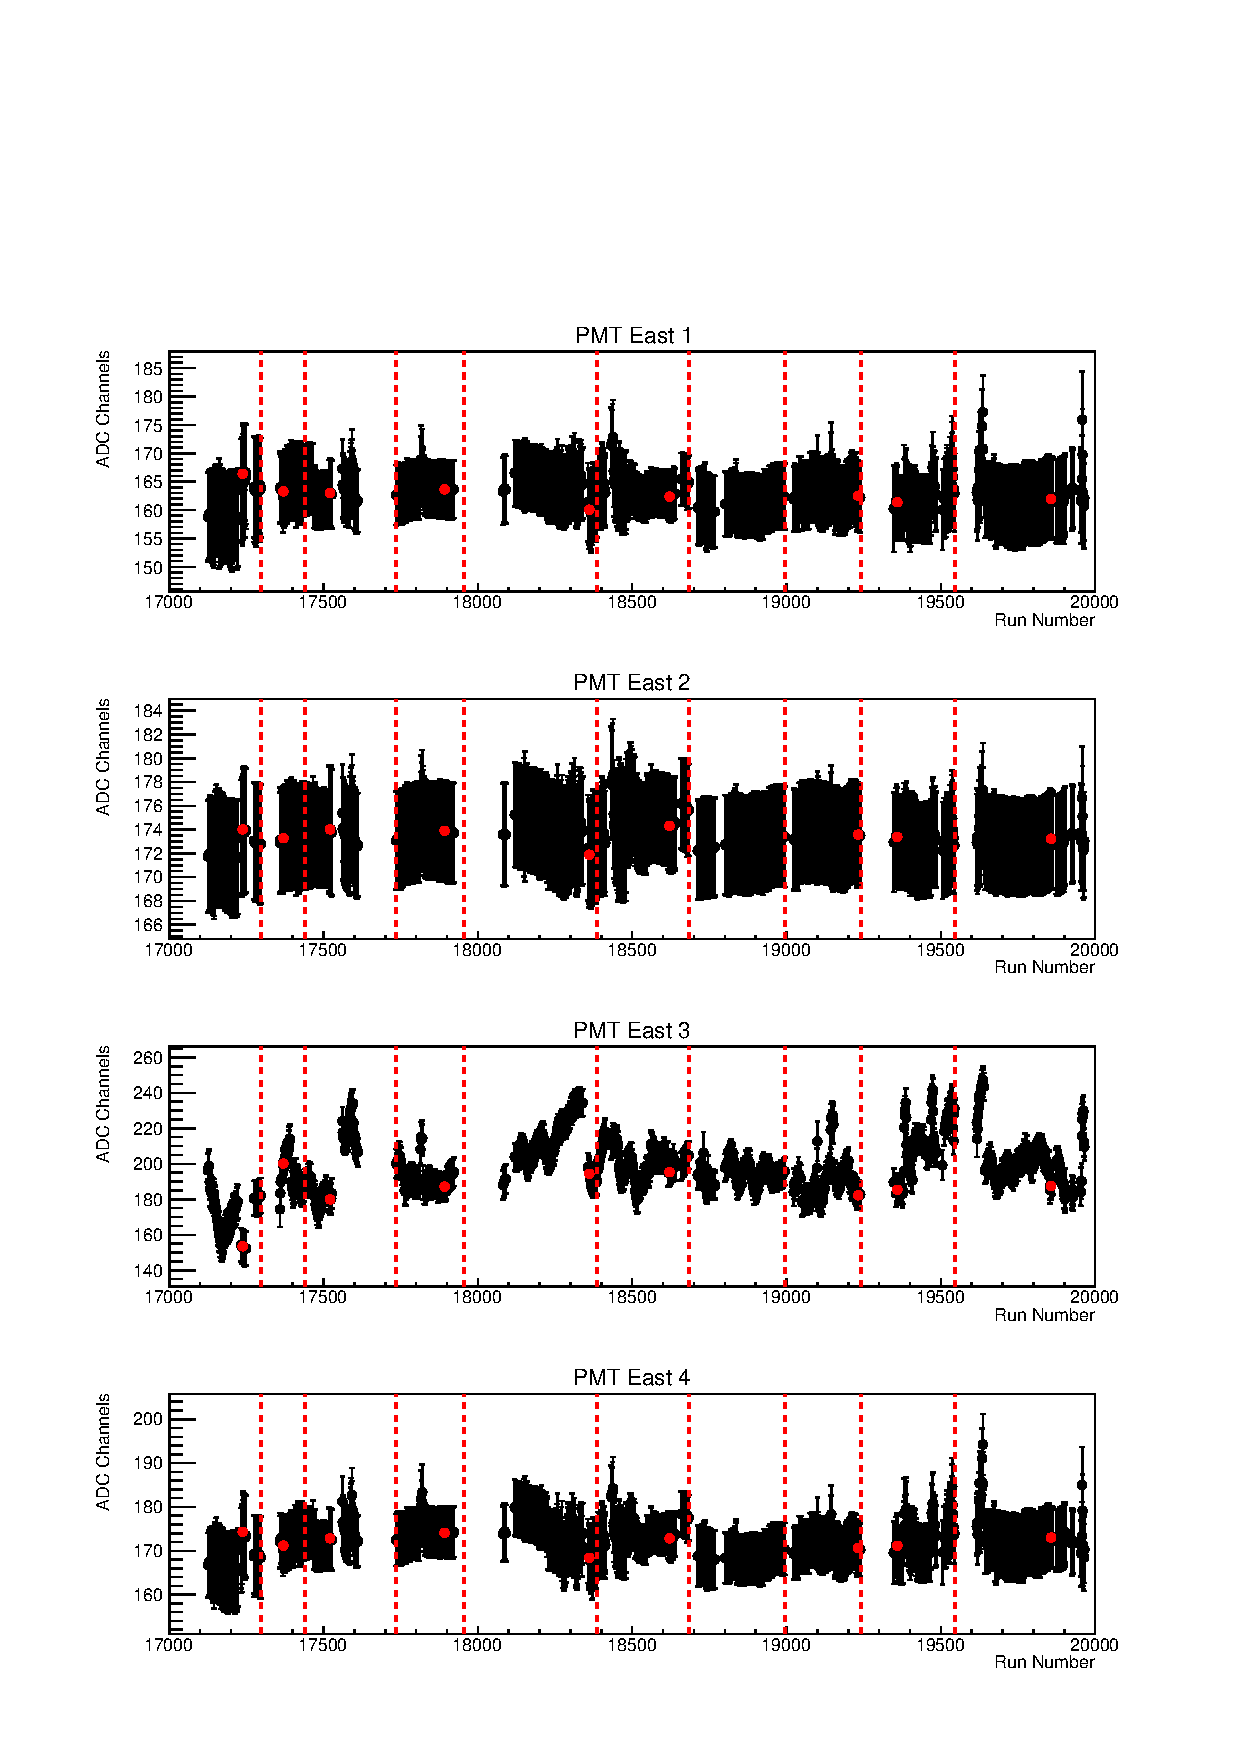
\includegraphics[page=1,scale=0.8]{3-UCNAAnalysis/2011-2012_pedestals.pdf}
\caption{Pedestal means as a function of run number for 2011-2012 East Detectors. Error bars are the
  RMS of the measured pedestal. The red lines indicate what ranges of runs belong to
  different calibration periods, and the red marker is the calibration reference run,
  which will be discussed in later sections. Missing periods of data indicate some sort of failure
  from that PMT, and so it was removed from the analysis over that period.}
 \label{fig:peds_timeDep}
\end{figure}

\begin{figure}[p] 
\centering
\includegraphics[page=2,scale=0.8]{3-UCNAAnalysis/2011-2012_pedestals.pdf}
\caption{Pedestal means as a function of run number for 2011-2012 West Detectors. Error bars are the
  RMS of the measured pedestal. The red lines indicate what ranges of runs belong to
  different calibration periods, and the red marker is the calibration reference run,
  which will be discussed in later sections. Missing periods of data indicate some sort of failure
  from that PMT, and so it was removed from the analysis over that period.}
\label{fig:peds_timeDep}
\end{figure}

One interesting thing to note is that the discriminators, which determine whether
a component triggers,
for all PMTs are housed 
together, which leads to correlations between the PMT triggers. In a perfect world, 
each PMT would have one pedestal, and that pedestal wouldn't care about other PMT's signals.
Instead, what we see is that the pedestals
can be dependent on the type of events that are chosen 
to construct the pedestal, and the effect can be \~10~channels for some PMTs.
This indicates that the pedestal for one PMT may be dependent
on the signal present in another PMT. These shifts are important as a
pedestal shift of 5-10 channels maps to an offset of roughly
5-10 keV, as the PMTs show close to 1:1 correspondence between ADC and keV.

The influence of event type on pedestal values means we must carefully choose which events
to use when calculating the pedestal.
The best choice would be UCN monitor events due to there being zero signal 
in the electronics box housing the PMT electronics, and these thus would give
the cleanest measurement of the PMT pedestal.
These are unfortunately the first event type we can eliminate as they are only present
during $\beta$-decay runs (when UCN are produced and thus create UCN monitor triggers)
and not during calibration runs (taken during the day when the beam is off). 
Of the remaining two options, the choice was made to use the
two-fold PMT triggers from the opposite detector rather than $^{207}\mathrm{Bi}$ pulser
events. The choice is somewhat arbitrary, because what is important is that we choose
a consistent subset of data for both calibration and $\beta$-decay data, but the
opposite side two-fold triggers do better represent the baseline present in each PMT
for data events when compared to the much higher signal present from the $^{207}\mathrm{Bi}$
pulser.


\iffalse
\begin{figure}[h] 
\centering

\includegraphics[scale=.25]{3-UCNAAnalysis/ImageHolder.pdf}
\caption{Pedestal values for a $\beta$-decay run determined using different 
types of events to illustrate the cross-talk between PMTs. (UCN Monitors, 
Bi triggers, Opposite side triggers, same side 2-fold triggers. Also shown 
is the dependence of the pedestal on which PMT triggers in the Bi Pulser. NOTE:
Choose West PMT4 in an early 2012/2013 beta run) }
\label{fig:peds_types}
\end{figure}

\begin{figure}[h] 
\centering

\includegraphics[scale=.25]{3-UCNAAnalysis/ImageHolder.pdf}
\caption{Example pedestals from all 8 PMTs}
\label{fig:peds_ind}
\end{figure}
\fi



With the event type chosen, we extract the mean and RMS of the pedestal peak
for each PMT in every run. The pedestal mean (referred to as simply
the pedestal) is then subtracted from the ADC values for all events. This effectively
removes the time-dependent baseline from the detector signals. The time dependence of
the pedestals can be seen for the East PMTs from 2011-2012 in Figure \ref{fig:peds_timeDep}.
Most of the PMTs have pedestals which remain quite stable, but PMT East 3 shows the
importance of a run-by-run pedestal subtraction.



\subsection{Gain Correction} \label{ssec:BiGain}

\subsubsection{$^{207}\mathrm{Bi}$ Pulser}
%The goal of the $^{207}\mathrm{Bi}$ gain monitoring pulser system is to create a standard
%candle type signal present in all PMTs to be tracked over time. 
The primary gain monitoring system consists of a small amount $^{207}\mathrm{Bi}$
deposited within a small block of scintillator. The scintillator was surrounded by
light reflecting material on three sides, with the fourth side covered with an optical
attenuator to attempt to match the light output of the $\sim$1~MeV conversion line in the $^{207}\mathrm{Bi}$
to the light output of 1~MeV of energy deposited in the detector scintillator. The pulser was then
attached directly to the PMT next to where the light guides attached to the PMT.
To allow for a single-PMT high threshold trigger, the signal was split off to a different
discriminator than the one used when determining a two-fold trigger. These high threshold
discriminators then allowed for pulser triggers with a distinct pulser identification \cite{mpmThesis}.

An unfortunate but low impact issue with the pulser involves the amount of attenuation applied to the
pulser signal. The pulser peak lies well beyond the equivalent of 1~MeV of light as would be produced
in the detector scintillator, and therefore far outside the range of the $\beta$-decay spectrum. This
is not a serious issue as the PMTs seem to be quite linear, so even a peak well outside the
energy range of interest should suffice.

\begin{figure}[h] 
\centering
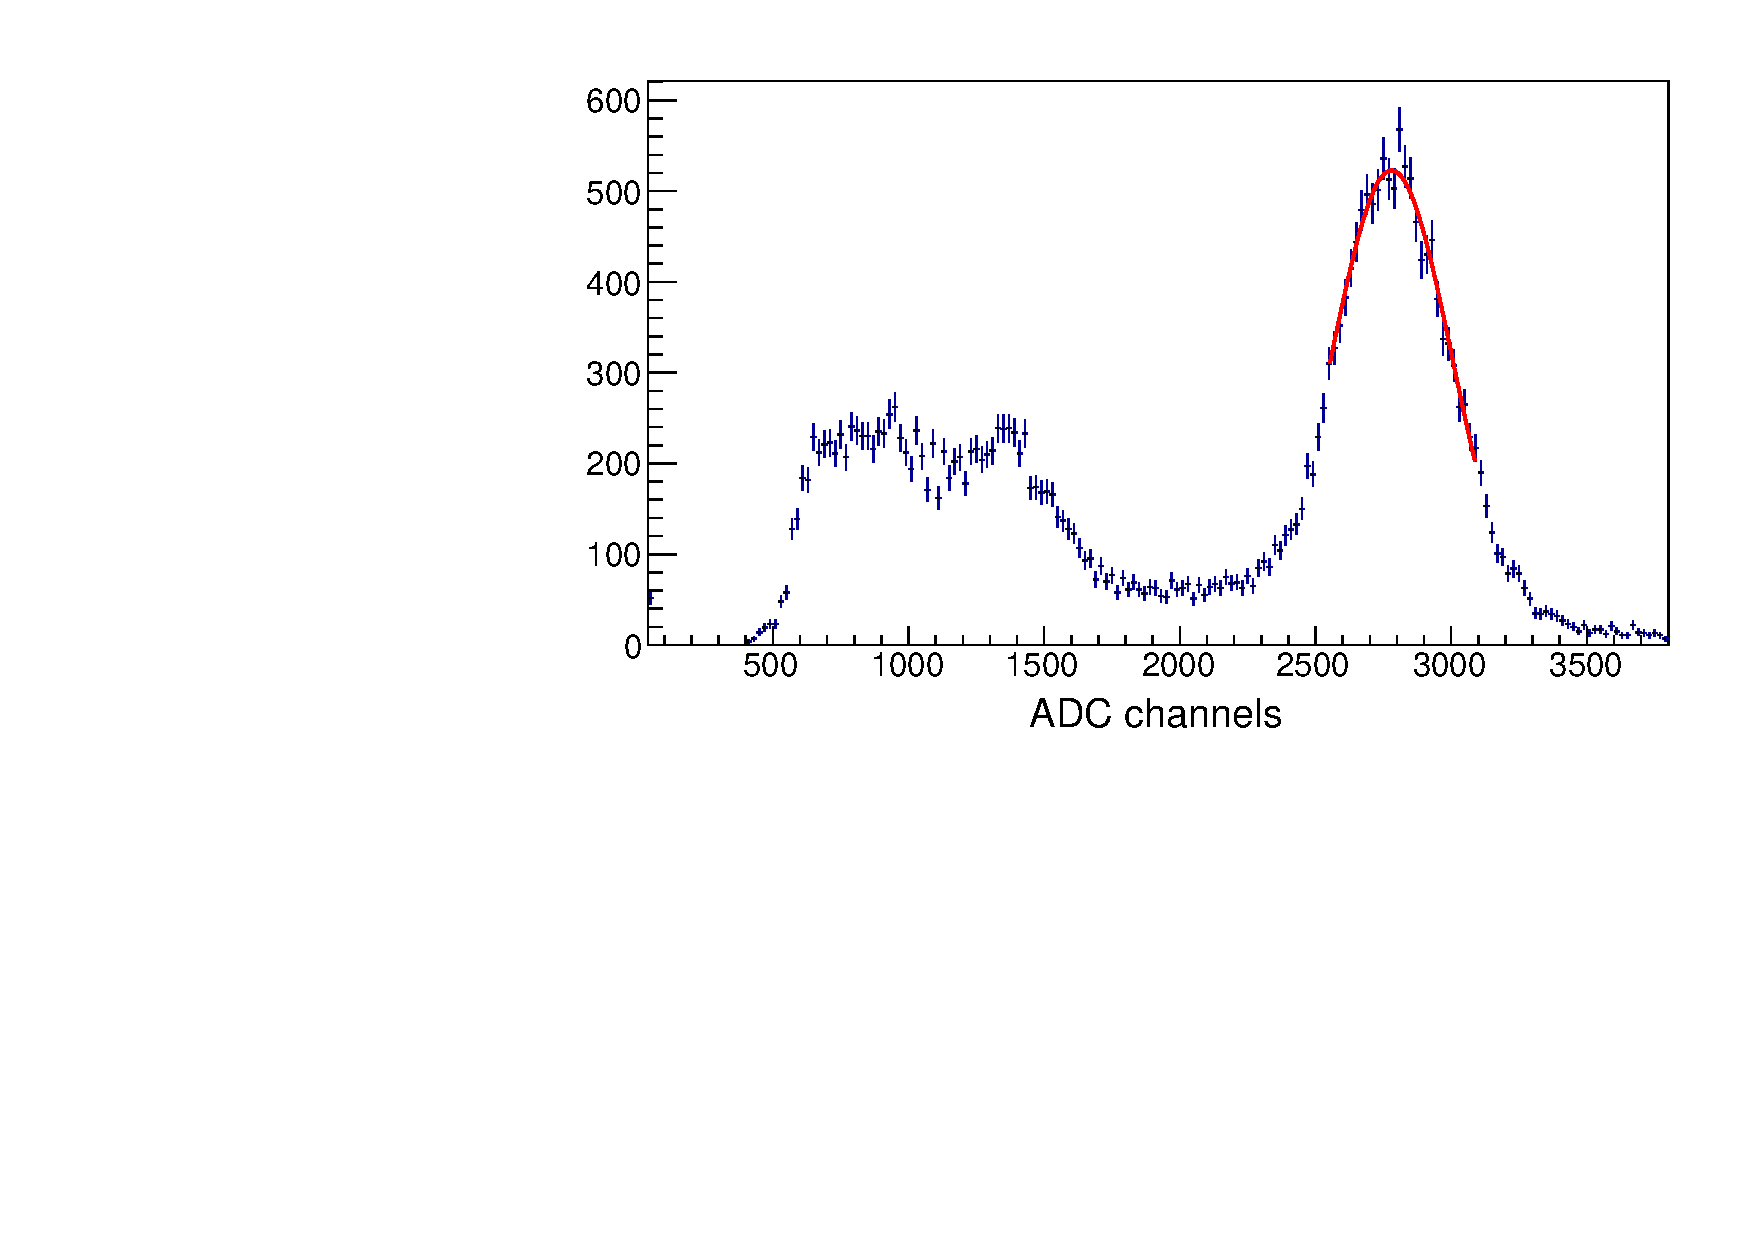
\includegraphics[scale=.60]{3-UCNAAnalysis/gain_bismuth2.pdf}
\caption{Example $^{207}\mathrm{Bi}$ spectrum and fit for a single PMT over
  the course of a run. The upper and lower bismuth conversion electron peaks are
  seen, along with a distribution from decay gammas. Note that the gamma rays are
  visible because the pulser is attached directly to the PMT and there is no type
  of veto (like the MWPC) to remove them.}
\label{fig:biPulser}
\end{figure}

The $^{207}\mathrm{Bi}$ pulser peak is fit by a Gaussian on a run-by-run basis, allowing for gain corrections on the time
scale of a single run. The fit was done iteratively, with the initial guesses for mean and fit range determined
by stepping backwards from the last bin and using a self-written algorithm to search for the peak. Then the peak
was fit five times consecutively, with each successive fit being fed the previous fit's mean and sigma. This
made sure the fit converged as best as possible on the mean of the pulser peak. An example pulser peak and fit
can be seen in Figure \ref{fig:biPulser}. The asymmetric fit (range extends farther above the peak than below)
is actually a characteristic part of the iterative
fitting algorithm developed for use throughout this analysis. For Gaussian like peaks occurring as a result of
a process like energy loss in a scintillator followed by PMT amplification, the upper end of the peak is
inherently more Gaussian due to the lower end having a tail from extraneous energy losses. 

The method for applying the gain correction is as follows. First, a reference gain must be determined
to normalize all other gains against. This was chosen to be what is called the ``reference run'', and it
typically consists of a manually inspected source run within each source calibration period. The gain factor
is then calculated as the ratio of the pulser peak in a given run divided by the pulser peak in the reference
run, or
%
\begin{equation}
  g_i = \frac{\mu_i}{\mu_{\mathrm{ref}}}
\end{equation}
%
This automatically defines the gain of the reference run to be $g_{\mathrm{ref}}=1$. Then all other runs which are
calibrated by a certain run period have gain factors which vary based on the fitted pulser value. The time
dependence of the gain values in 2011-2012 can be seen in figures \ref{fig:2011-2012pulser_East}
and \ref{fig:2011-2012pulser_West}. The behavior is similar in 2012-2013.

Some problems with the $^{207}\mathrm{Bi}$ pulser did occur. There were several periods where the pulser
simply did not work for a certain PMT. This was always limited to a single PMT not working at a given time, and when this
was the case the PMT without a pulser signal was not used when reconstructing the energy. This has
minimal effect on the energy reconstruction though, as the ``bad'' PMT is still used when determining
a two-fold trigger, and the remaining three PMTs contain sufficient information for reconstructing the
energy deposited. Periods where $^{207}\mathrm{Bi}$ pulser information is missing are evident in
Figure \ref{fig:2011-2012pulser_West} where there is missing data for certain PMTs over extended ranges.
It should be noted that in 2012-2013, West PMT4 never had a functioning pulser and was never used for
energy reconstruction purposes.

\begin{figure}[p] 
  \centering
  \includegraphics[page=3,scale=.8]{3-UCNAAnalysis/2011-2012_gain.pdf}
  \caption{Gain factors, $g_i$, as a function of run number for 2011-2012 East Detectors.
    The red lines indicate what ranges of runs belong to
    different calibration periods, and the red marker is the calibration reference run.}
  \label{fig:2011-2012pulser_East}
\end{figure}

\begin{figure}[p] 
  \centering
  \includegraphics[page=4,scale=.8]{3-UCNAAnalysis/2011-2012_gain.pdf}
  \caption{Gain factors, $g_i$, as a function of run number for 2011-2012 West Detectors.
    The red lines indicate what ranges of runs belong to
    different calibration periods, and the red marker is the calibration reference run.}
  \label{fig:2011-2012pulser_West}
\end{figure}

\subsubsection{Endpoint Stabilization} \label{sssec:endpoint}

There are unexplained longer term gain fluctuations that do not seem to be captured by the
$^{207}\mathrm{Bi}$ gain monitoring system that can be seen by monitoring the endpoint of the
$\beta$-decay spectrum. These are corrected by applying a second gain factor, $g_{\mathrm{ep},i}$ for PMT $i$,
as the last step in the calibration process. This endpoint gain factor is determined
by comparing the endpoints as seen by each
calibrated PMT to the expected endpoint from the simulation. The final energy for each PMT
is then multiplied by this factor. This does not force the final reconstructed energy endpoint to
match the final reconstructed simulation endpoint exactly,
as the final spectra are the weighted average of the four PMT responses, but rather it corrects 
some systematically shifted periods of data which consistently exhibited endpoints $>30$~keV
away from the expected endpoint.

The method for calculating $g_{\mathrm{ep}}$ was developed previously by M. Mendenhall in section
5.2.2 of \cite{mpmThesis}. For the sake of clarity, the process is repeated here.

\begin{figure}
  \centering
  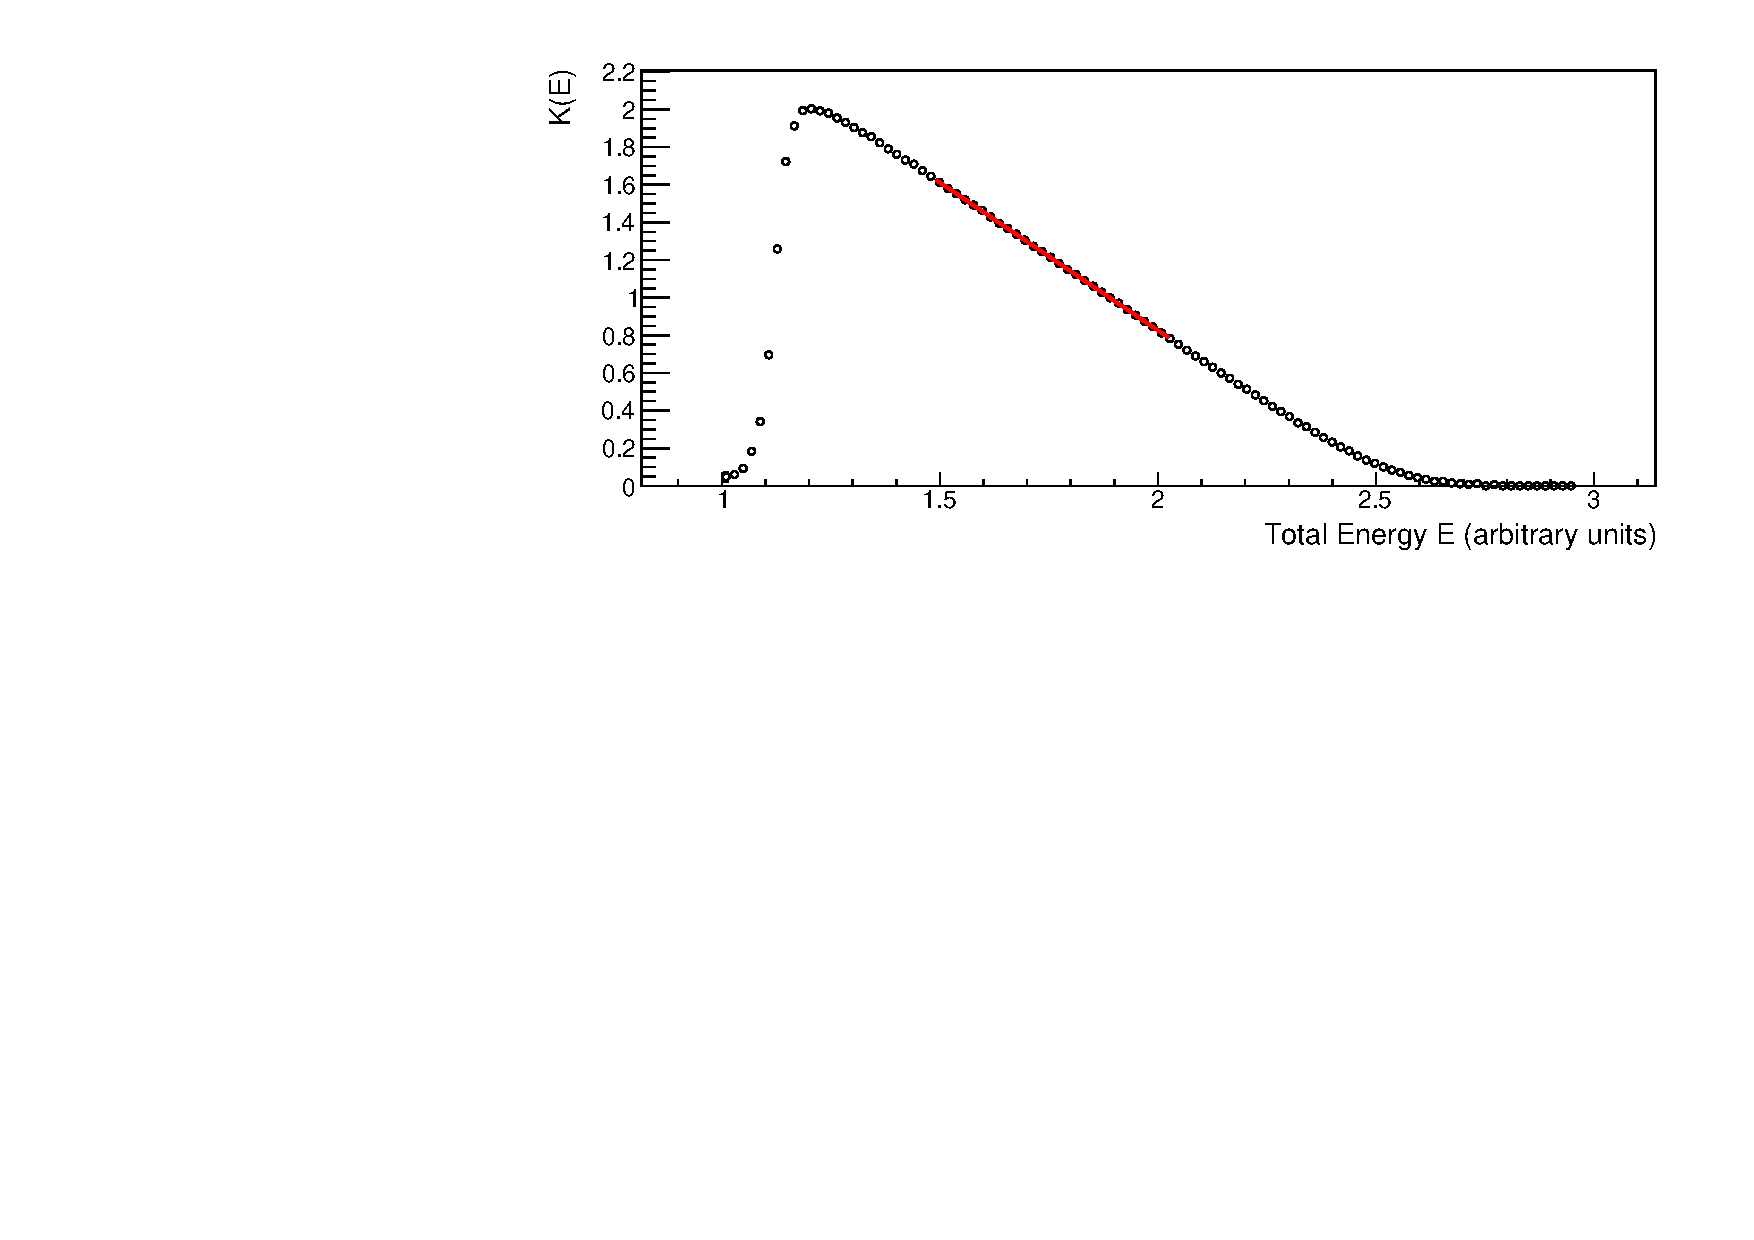
\includegraphics[scale=0.75]{3-UCNAAnalysis/kuriePlot.pdf}
  \caption{Example Kurie plot with linear fit to extract the y-intercept, which is
    the endpoint energy. The deviations from a straight line are due to the
    trigger efficiency at low energies and finite resolution at high energies. Care
    must be taken to fit in a region which more appropriately characterizes the true
    underlying electron energy spectrum.}
  \label{fig:kuriePlot}
\end{figure}
  

The endpoints are fit using a Kurie plot \cite{kurie1936radiations}, which linearizes the
energy response making for easy determination of the endpoint energy. If we approximate
the decay rate as the phase space factor for the neutron, then we can write down
the decay rate as a function of the electron total energy $E$, endpoint
energy $E_0$, and momentum $p$ as
%
\begin{equation}
  S(E) = pE\big(E_0-E\big)^2
\end{equation}
%
From this we see that a linear equation (the Kurie plot) can be formed:
%
\begin{equation}
  K(E) = \sqrt{\frac{S(E)}{pE}} = E_0-E
\end{equation}
%
where the $y$-intercept and $x$-intercept both determine the endpoint energy $E_0$.
An example Kurie plot can be seen in Figure \ref{fig:kuriePlot}.

Now we assume that the measured kinetic energy spectrum $T_{\mathrm{meas}}$ is different from the expected
kinetic energy spectrum $T_{\mathrm{sim}}$ by the gain factor $g_{\mathrm{ep}}$ such that
%
\begin{equation}
  T_{\mathrm{sim}} = g_{\mathrm{ep}} T_{\mathrm{meas}}.
\end{equation}
Then we can write the
measured total energy as
\begin{equation}
  E_{\mathrm{meas}} = m_e + g_{\mathrm{ep}}T_{\mathrm{meas}} \quad (c=1).
\end{equation}
The extracted endpoint for the data is now a function of $g_{\mathrm{ep}}$
since
\begin{equation}
  K(E_{\mathrm{meas}}) = \sqrt{\frac{S(E_{\mathrm{meas}})}{pE_{\mathrm{meas}}}} = E_{0,\mathrm{meas}}-E_{\mathrm{meas}},
\end{equation}
and upon proper choice of $g_{\mathrm{ep}}$, $E_{\mathrm{meas}}=E_{\mathrm{sim}}$. To solve for
the proper gain factor, the data endpoint is iteratively fit with the gain factor adjusted upon each iteration
according to
%
\begin{equation}
  g'_{\mathrm{ep}} = \frac{ E_{0,\mathrm{meas}}- m_e}{ E_{0,\mathrm{sim}}- m_e}g_{\mathrm{ep}} =  \frac{ T_{0,\mathrm{meas}}}{ T_{0,\mathrm{sim}}}g_{\mathrm{ep}}, 
\end{equation}
%
where $E_{0,\mathrm{meas}}$ is the extracted endpoint energy from the data with gain factor $g_{\mathrm{ep}}$ applied,
$E_{0,\mathrm{sim}}$ is the expected endpoint energy extracted from simulation, $T_0$ is the endpoint kinetic energy,
and $g'_{\mathrm{ep}}$ is the guess for the next iteration of endpoint fitting.
Once the condition $1-\frac{g'_{\mathrm{ep}}}{g_{\mathrm{ep}}}<10^{-7}$ is met, the value of $g'_{\mathrm{ep}}$ is taken as the final
endpoint gain factor and is saved to the calibration database. This process is carried out for each PMT for every
$\beta$-decay run, and then every event is reprocessed with the new gain factor applied to the visible energy from PMT
$i$ according to
%
\begin{equation}
  E_{\mathrm{vis},i}^{\mathrm{FINAL}} = g_{\mathrm{ep},i} E_{\mathrm{vis},i}.
\end{equation}
Then $E_{\mathrm{recon}}$ is calcuated using the final visible energies from the available PMTs.



\subsection{Time-dependent backgrounds}
Background events which may have some time dependence are removed from the analysis
via dedicated background runs that accompany every $\beta$-decay run.
Subtracting these background rates from the data rates accounts for backgrounds
with roughly a one hour time variation.
Any backgrounds that vary at the sub one hour level may go unnoticed, but
with a signal to background better than 50:1 the contribution from such is minimal.
Background subtraction will be addressed in Section \ref{sssec:bgsubtr}. 

\section{Trigger Thresholds} \label{sec:triggerThresh}

Looking ahead to the detector response model that will be implemented when processing
the simulated data, we need to determine the trigger thresholds for each of the
PMTs. With each PMT attached to a leading edge discriminator, the
amount of charge in a pulse that can create a trigger is randomized. The ADC signal
is an integrated signal, so two signals with integrated charge
at roughly the trigger threshold may have
different amplitudes and therefore different likelihoods of passing the discriminator threshold.
Measurement of these thresholds is important for the detector response model within the simulation
in order to properly model the low energy behavior of the measured spectrum.


\subsection{General Model for Trigger Determination} \label{ssec:genTrigModel}

The most important part of determining the trigger threshold shape for 
any detector is the availability of data which was collected no matter if 
the detector produced a trigger. If such a subset of 
data is available and plentiful, it is straightforward to estimate
the trigger probability by binning the data in some unit proportional to 
energy (whether in energy or something like it is not important) and taking 
the bin-by-bin ratio of those events that triggered to all of the events in the 
sample. Plotting these ratios as a function of whatever energy-like metric was chosen tells 
you how probable an event of some value is to create a trigger.
Once you have mapped this probability, you can then sample these curves within 
simulation to apply your true trigger threshold to simulated data.


\subsection{Trigger Data Selection}
As mentioned before, the data used for constructing trigger thresholds must not be 
biased towards triggering the PMT of interest. Thus that PMT must not be a mandatory 
component of the global trigger for that event, and care must be taken to choose only 
events which would trigger regardless of the behavior of the PMT of interest. One
other stipulation placed on these events is that they have an opportunity to 
deposit energy in a particular scintillator. The best choice of events that 
satisfy these conditions are those that have a two-fold trigger on the opposite side 
and then backscatter and those that trigger at least three PMTs on the side of 
interest, which guarantees that the scintillator would have triggered with or without 
the PMT of interest.	

\subsection{Determining the Trigger Probability}
One option for determining the trigger probability function (and probably the 
most straightforward) is to calculate the trigger probability for an entire detector as 
a whole as a function of the energy deposited by an event. What you get is a 
function that provides the probability that an event of energy $ E_i $ 
produces some sort of trigger in that 
detector. Initially this method was employed in this analysis for sake of simplicity, and it produced 
reasonable agreement between simulation and data, but there is one 
glaring concern: Determining this trigger function from data requires that the data be 
calibrated first. At first glance this may not seem like much of an issue, but the 
calibration hinges upon the 
simulated peaks at low energy, which in turn rely on the trigger functions. This 
cyclical dependence hinders one from truly understanding any discrepancy between 
simulation and data at low energies, which is exactly the reason this method was 
abandoned.  

Instead, similarly to previous analyses, we decided to calculate the trigger
function on a PMT-by-PMT basis as a function of ADC channels above pedestal. This
encompasses a true characteristic of each component of the detector rather than some
average effect as seen by a detector package, which is what the aforementioned 
method produces. A typical trigger threshold is seen in Figure \ref{fig:trigger_thresh}.
As illustrated in Section \ref{ssec:genTrigModel}, the ratio of triggering events
to all events was taken in each ADC bin and then fit using the method described
in the following section.
  

\begin{figure}[h] 
\centering
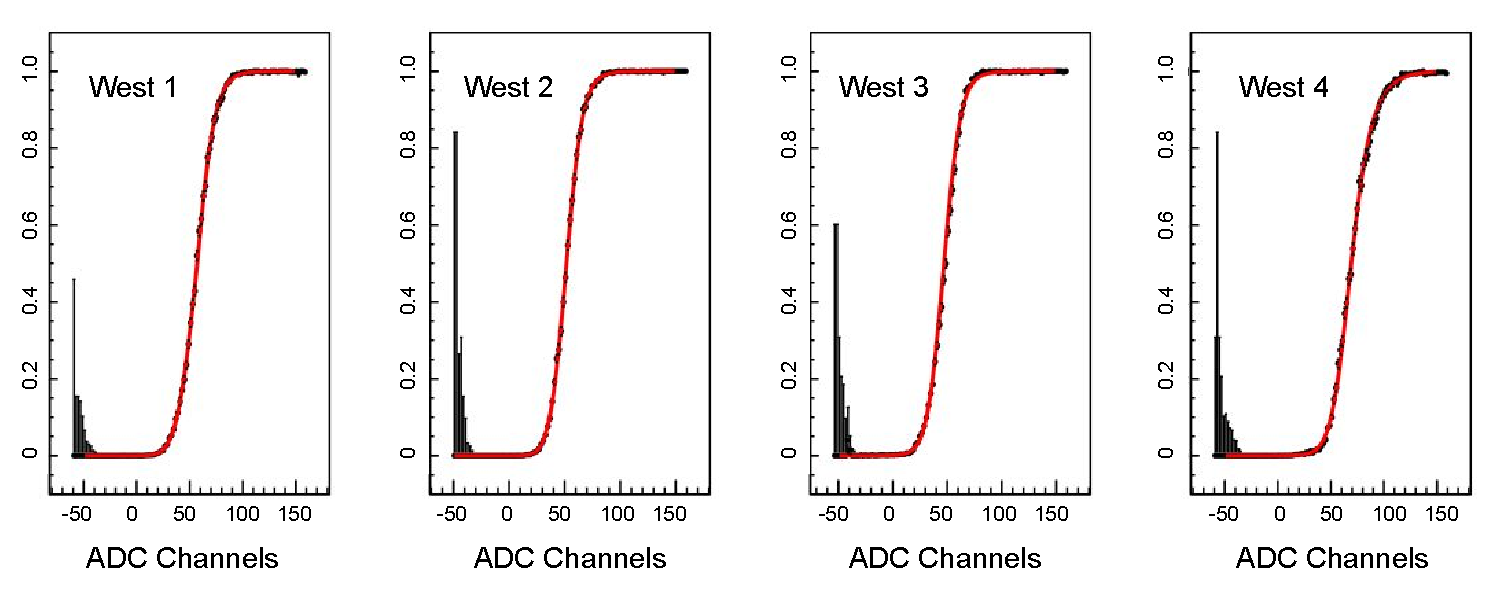
\includegraphics[scale=.6]{3-UCNAAnalysis/triggerThresholds.pdf}
\caption{Typical trigger thresholds as a function of pedestal subtracted
  ADC values from the West PMTs with fits shown in red. The y-axis
  is a probability of triggering given some ADC signal.}
\label{fig:trigger_thresh}
\end{figure}

\subsubsection{Functional Fit of the Trigger Threshold}
From the sigmoid shape of the threshold data in Figure \ref{fig:trigger_thresh}, one might guess
the shape of the curve to be a hyperbolic tangent or an error function. The data tends to show
a sharper turn on at lower ADC channels and a softer leveling off to unit probability, which
prompted the use of both the $\mathrm{erf}(x)$ (lower end of transition region)
and $\tanh(x)$ (upper end of transition region),
with a continuous transition between the
two provided by a smoothing function $S_\pm$ defined as
%
\begin{equation}
  S_\pm\big(x;x_0,R\big) \cdot f(x) = \frac{1}{2}\bigg(1\pm\tanh\Big(\frac{x-x_0}{R}\Big)\bigg) \cdot f(x),
\end{equation}
%
which acts to ``turn on/off'' ($+/-$) a function $f(x)$ around the pivot point $x_0$ and with the severity of
the on/off transition determined by the width parameter $R$. The functional fit $F(q)$ then becomes (note that the $\mathrm{erf}(x)$ and $\tanh(x)$ 
have the range (-1,1), so they must be shifted and the range halved to accomodate $0<F(q)<1$):
%
\begin{equation}
  F(q) = \frac{1}{2} \Bigg[ S_-\big(q;\mu,R\big) \bigg(1 + \mathrm{erf}\Big(\frac{q-\mu}{w_1}\Big)\bigg) +
  S_+\big(q;\mu,R\big) \bigg(1+\tanh\Big(\frac{q-\mu}{w_2}\Big)\bigg)\Bigg]
\end{equation}
%
where $q$ is the ADC value and
the free parameters are $\mu$ ($f(q=\mu)\approx 0.5$), $w_1$ (width of $\mathrm{erf}$), $w_2$ (width of $\tanh$), and $R$ (severity of turn on/off).
This function, while motivated purely by inspection of the shape of the trigger threshold, fits the data
quite well with only these four free parameters. An example of the fits for a single $\beta$-decay
run can be seen in Figure \ref{fig:trigger_thresh}. 

%-----------------------------------------------------------


\section{Simulation}
\label{sec:Simulation}

For this work, the simulation software from previous analyses was adopted
and modified where seen fit to accomodate changes in the geometries
and materials. The finer details of the particle generation and
tracking can be found in \cite{mpmThesis}. For our purposes, a summary
of the important quantities is more than sufficient for understanding
the work contained within this thesis.

\iffalse The simulations and application of the
detector response model provide a suitable starting
point for discussing the analysis, as the calibration of the data hinges
strongly on the simulation results. There is a notable dependence of the
response model on data, but this will be addressed as needed
when describing the calibration.

The simulation work for this thesis was completed
using the Geant4 simulation software package. The geometry of the
apparatus was duplicated
to the best precision possible and benchmarked against data after
the detector response model was applied. The structure
of the simulation code did not change from those in the previous analysis
as described in \cite{mpmThesis}, although minor changes were
made to the geometry to reflect real adjustments to the experimental
apparatus. \fi

\subsection{Overview}

The simulation of the experimental geometry and particle tracking was completed
using the \textsc{Geant4} Monte Carlo particle transport software package
\cite{agostinelli2003geant4}. The initial kinematics of the event vertices
were determined pre-simulation and fed into the \textsc{Geant4} toolkit, at which
point the particle was propagated via Monte Carlo sampling of interactions
with all components of the experimental geometry, including the magnetic field.
The energy deposition was recorded within all sensitive detector components and
even within the decay trap windows and walls, to which we do not have access
in the real data. The relative timing of the scintillator hits was also
recorded so as to mimic the timing signals of the experiment.

The simulation is especially important when determining systematic corrections due
to a priori knowledge of the initial kinematics of each event. Thus, after an event
comes to rest and its detector response is considered, one can compare the signature
of the signals to the initial momentum of the particle and analyze possible
effects on observables from backscattering, angular dependence, and energy losses
in non-sensitive detector regions for example.

\subsection{Geometry and magnetic field} \label{sssec:simMagField}

The geometry input into the \textsc{Geant4} simulation is taken directly from
that given in Chapter \ref{ch:UCNA_Experiment}. Options for each variation
of the geometry were implemented, including a 2011-2012 option with
the thicker decay trap endcaps and a 2012-2013 option with thinner asymmetric
decay trap endcaps. The 2012-2013 geometry is further subdivided into an option
for neopentane in the wirechamber (same as 2011-2012) and for isobutane in the
wirechamber, as a portion of the 2012-2013 runs were taken with this
different fill gas. Any other minor differences in the geometry were also
incorporated into the detector construction.

The magnetic field profile is nominally taken to be 1~T in the decay trap
with the field expansion to 0.6~T at the wirechambers incorporated also.
Options to use the measured field maps, one of which is depicted in
Figure \ref{fig:field_profile}, were included, but in all source
and $\beta$-decay simulations the smooth profile was used to save on
computation time. Effects on the asymmetry from the non-smooth
field profile present during data taking is addressed in
Section \ref{sssec:MagFieldSyst}.

The magnetic field is passed to the simulation as a set of discrete $B_z$
values along the $z$-axis of the spectrometer as depicted in Figure \ref{fig:field_profile}.
The continuous field profile on the $z$-axis is then interpolated between consecutive $z_i$ locations
using the respective $B_z(z_i)$ values by a half-wave of a cosine,
%
\begin{equation}
  B_z(z) = \frac{B_z(z_i) + B_z(z_{i+1})}{2} + \frac{B_z(z_i) - B_z(z_{i+1})}{2}\cos\bigg(\frac{z-z_i}{z_{i+1}-z_i}\pi\bigg),
\end{equation}
%
where $z_i<z<z_{i+1}$.

Then, if the field is taken to be azimuthally symmetric ($B_\phi(z,r,\phi)=0$) and $B_z(z,r,\phi)=B_z(r)$,
the $r$-component can be calculated from Maxwell's equations:
%
\begin{equation}
  \nabla \cdot \vec{B} = 0 \Rightarrow \frac{\partial B_z}{\partial z} + \frac{1}{r}\frac{\partial}{\partial r}\big(rB_r\big), 
\end{equation}
\begin{equation}
  B_r(z,r) =  \frac{B(z_i) - B(z_{i+1})}{z_{i+1}-z_i}\frac{\pi r}{4}\sin\bigg(\frac{z-z_i}{z_{i+1}-z_i}\pi\bigg).
\end{equation}
%


\subsection{Event Kinematics}

\subsubsection{Conversion Electron Sources}
For the conversion electron sources, the decay probabilities for conversion electrons,
Auger electrons, and gamma rays are read from files specific to each isotope.
The energy and radiation type sample the decay chain probabilities from these files, and
the momentum is chosen isotropically over 4$\pi$. The initial vertex for any source
event is randomly sampled within a small dot encapsulated in a sealed source holder
along the center axis of the decay trap, as would be the case for a real sealed
source used in the calibration.

\subsubsection{Neutron $\beta$-decay Electrons} \label{sssec:betaSim}

A detailed account of the functional form of the unpolarized $\beta$-decay rate used in the
event generator
is given in \cite{mpmThesis}. The corrections to the plain phase space spectrum are taken from
Wilkinson's series of review articles on $\beta$-decay
\cite{wilkinson1982,wilkinson1989evaluation,wilkinson1990evaluation,wilkinson1993evaluation,
  wilkinson1995evaluation,wilkinson1997evaluation,wilkinson1998evaluation} and include
the Fermi function coulomb correction, corrections for finite size of the nucleon, radiative
corrections as described in Section \ref{sssec:RadCorr}, and recoil corrections for the finite
mass of the proton in the final state.

For this analysis, the decays were sampled from a polarized spectrum, thus necessitating the
addition of the asymmetry to the decay rate. The polarized decay rate then took the form:
\begin{equation}
  \Gamma^{\mathrm{pol}}_\pm(E) = \Gamma^{\mathrm{unpol}}(E_e) \bigg( 1 \pm \xi(E) \bigg),
\end{equation}
where
\begin{equation}
  \xi(E) = A(E)\Big(1+\mathrm{R.O.}(E)+\mathrm{Rad}(E)\Big),
\end{equation}
$A(E)=A_0\beta cos\theta$, ``R.0.'' and ``Rad'' are the recoil order and radiative corrections to the asymmetry
consistent with those from Sections \ref{sssec:ROCorr} and \ref{sssec:RadCorr}, $\pm$ indicates the two possible spin states,
and $\Gamma^{\mathrm{unpol}}$ is the unpolarized
spectrum. The value of $A_0= -0.1184$ was used, as this is the current global average \cite{pdg}.

Each spin state was simulated for the 2011-2012 geometry, 2012-2013 geometry with neopentane in the wirechamber,
and 2012-2013 with isobutane in the wirechamber. Matching the proper spin state simulation to the polarization orientation
in the $\beta$-decay runs allows one to analyze the simulated data identically to the data. By comparing the
extracted asymmetries to the input value of $A_0$, we can ensure that the analysis method is at least internally
consistent.

A special thanks is in order for X. Sun for his contributions to the polarized event generator.

\subsection{Output}
The \textsc{Geant4} simulation provides trajectory tracking along with
the energy deposition along these tracks. Prior to processing the simulation
for calibration or systematic purposed, the first
task is to construct observables that are more useful.

\subsubsection{Energy Deposition}
By tallying the energy deposited along an entire track within some subset
of the geometry, one can reconstruct the energy deposited anywhere within
the SCS. The areas of primary interest for the sake of analysis are the
wirechambers and the scintillators. The energy deposited in the scintillator
is of highest importance, as the systematic studies depend on scintillator
reconstructed energy.  From here on,
the energy lost in the scintillator, as determined from summing the energy loss in simulation, will be
referred to as $E_{\mathrm{dep}}$. This is the maximum energy which could be detectable
for an event if no inconspicuous energy losses existed.

\subsubsection{Quenched Energy} \label{sssec:Equenched}
In reality, the energy that is visible in the form of scintillation light is not exactly
equal to $E_{\mathrm{dep}}$, but rather some of the energy is ``quenched'' when
the energy deposition per unit length grows large near the end of a track. The
empirical description for the light output by a charged particle traversing a
scintillator is given by Birk's Law \cite{birks1951scintillations}:
%
\begin{equation}
  \frac{dL}{dx} = S\frac{\frac{dE}{dx}}{1+k_B\frac{dE}{dx}},
\end{equation}
%
where $dL/dx$ is the light output per unit length, $dE/dx$ is the energy deposited per unit
length, $S$ is the scintillation efficiency, and $k_B$ is Birk's constant which must be
determined through measurement. For small $dE/dx$,
$dL/dx \propto dE/dx$, which is the case for the majority of an electron's track inside the scintillator.
As the electrons slow down and become very low energy, $dE/dx$ increases drastically
and $dL/dx \approx S/k_B = constant$. It is precisely this quenching effect that creates the difference
between the deposited energy and energy that may be observed through scintillation light. The energy
proportional to $dL/dx$ will be called the quenched energy and is defined as
%
\begin{equation}
  E_Q = \int \frac{\frac{dE}{dx}}{1+k_B\frac{dE}{dx}}dx,
\end{equation}
%
with the integration performed over the entirety of the path.

\begin{figure}[h] 
\centering
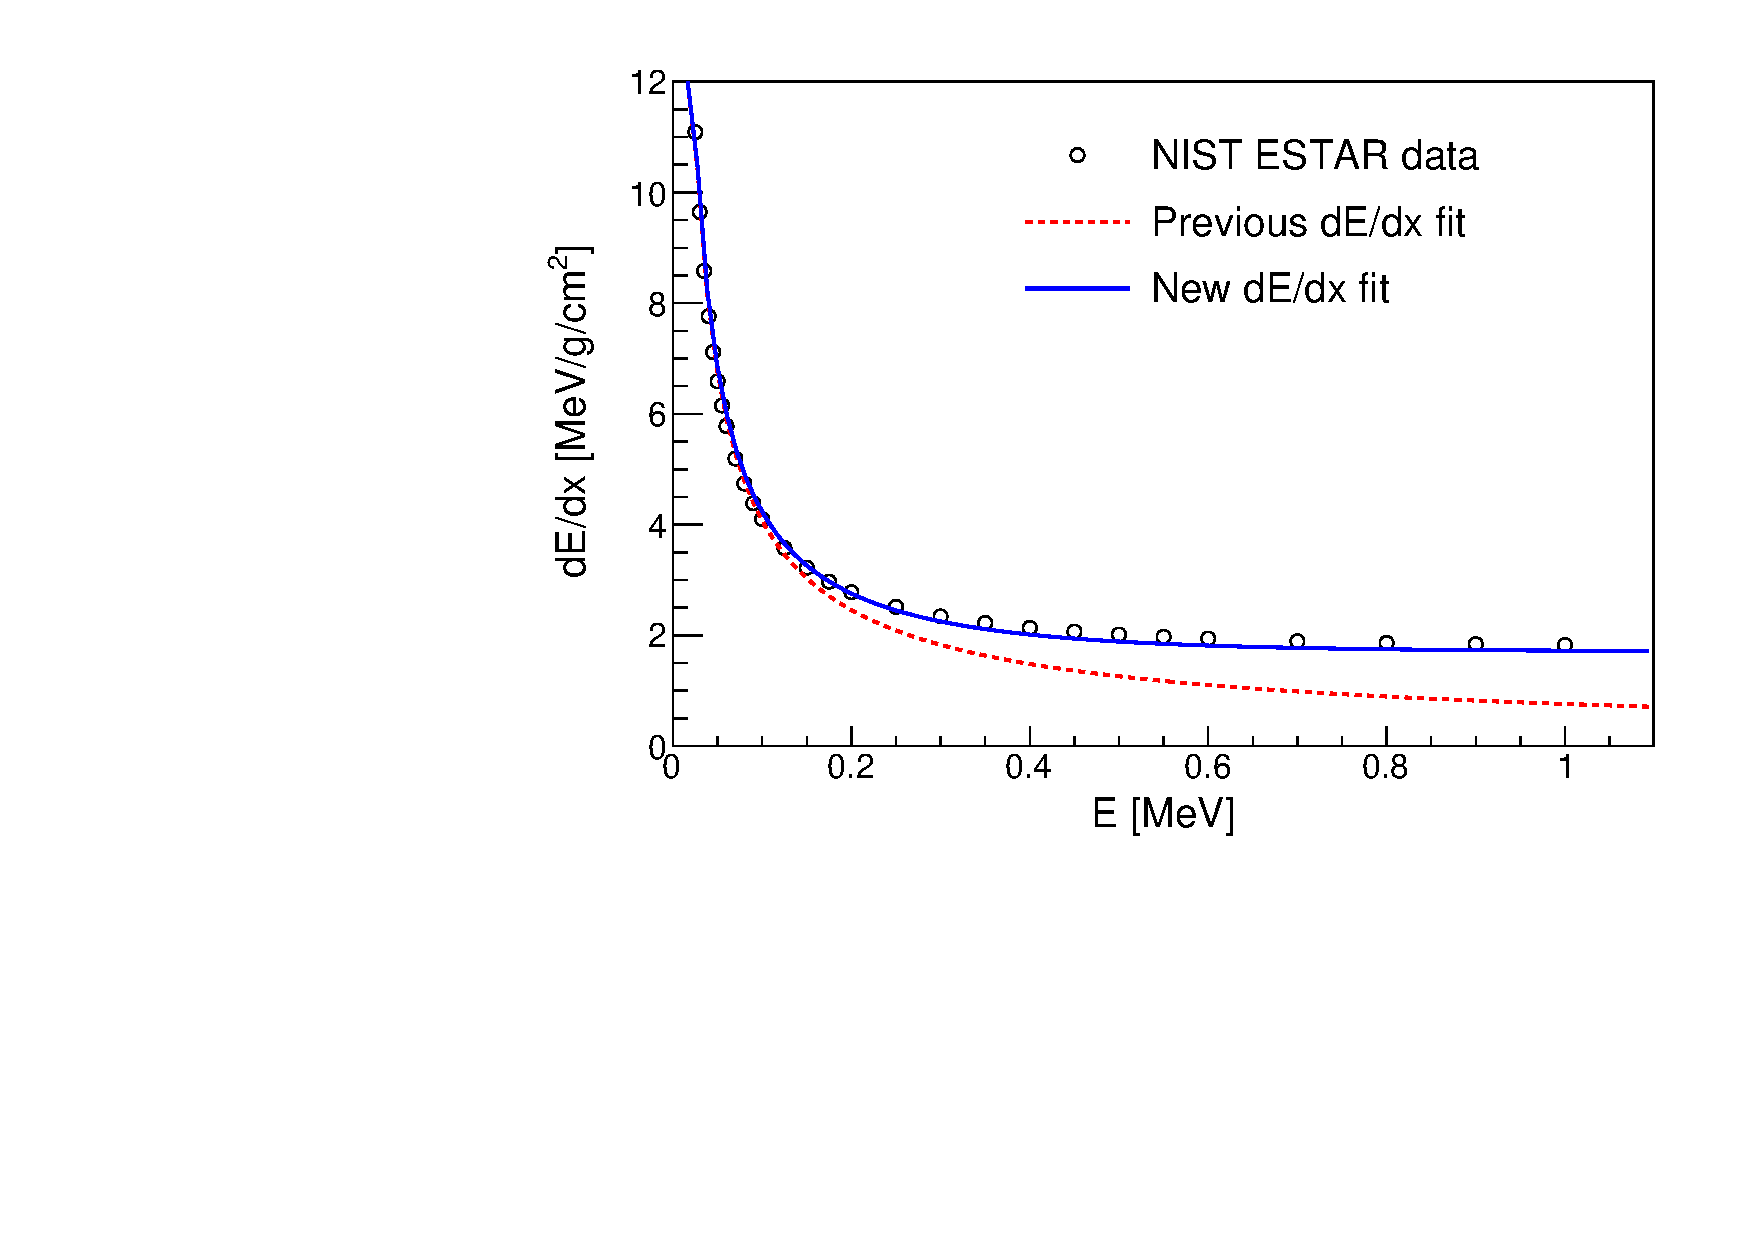
\includegraphics[scale=.6]{3-UCNAAnalysis/dEdx.pdf}
\caption{Plot of $dE/dx$ for a plastic scintillator. The data (open circles) comes from NIST ESTAR,
  and the dE/dx functional forms used previously (red dashed line) and presently (blue solid line)
  are shown.}
\label{fig:dEdx}
\end{figure}

In previous analyses, the functional form of $dE/dx $ was extracted from a fit to NIST ESTAR data
for a plastic scintillator \cite{yuan2006progress}. The fit determined the following relationship:
%
\begin{equation}
  \frac{dE}{dx} = 116.7\bigg(\frac{E}{\mathrm{keV}}\bigg)^{-0.7287} \rho_{\mathrm{scint}} \frac{\mathrm{MeV}}{\mathrm{g/cm}^2},
\end{equation}
%
where $\rho_{\mathrm{scint}}=1.032~\mathrm{g/cm}^2$ is the density of the scintillator. From
inspection of Figure \ref{fig:dEdx}, one can see that this expression for $dE/dx$ (red dashed line)
does not fit the data well at higher particle energy. Thus Dr. Brad Filippone suggested that the
functional form previously used be modified \cite{bradF_ELOG}:
%
\begin{equation}
  \bigg(\frac{dE}{dx}\bigg)_{\mathrm{new}} = \bigg(\frac{dE}{dx}\bigg)_{\mathrm{old}} + 1.35\big(1-e^{-0.00125\frac{E}{\mathrm{keV}}}\big) \rho_{\mathrm{scint}} \frac{\mathrm{MeV}}{\mathrm{g/cm}^2},
\end{equation}
%
which produces much better agreement with the data in Figure \ref{fig:dEdx}. The new $dE/dx$ was implemented for calculations
of $E_Q$ in the \textsc{Geant4} simulation for the current analysis with the value of $k_B=0.0191\pm0.0020$~cm/MeV as determined in
\cite{yuan2006progress}.




\subsubsection{Position of Detector hits}
The detector positions in both the scintillator and wirechamber are calculated as the weighted
average of the step positions, with the weights equal to the energy deposited in that step.
A more detector-like position response was utilized when analyzing the simulated data as is described
in Section \ref{ssec:simWirePos}, where the same position reconstruction algorithm used for data
is applied to simulated wirechamber responses.


%----------------------------------------------------------

\section{Energy Response from Detector Response} \label{sec:EnergyResponse}

The visible energy $E_{\mathrm{vis},i}$ deposited
in the scintillator as seen by a single PMT $i$ for an event at position $(x,y)$ 
is given by the following: 

\begin{equation} \label{eq:EvisResponse}
E_{\mathrm{vis},i} = \eta_i^{-1}(x,y) \cdot f_i\bigg( \Big( \mathrm{ADC}_i - p_i(t) \Big) \cdot g_i(t) \bigg)  ,
\end{equation}

\noindent where 
\begin{align*}
  f_i(\mathrm{ADC}) = & \text{ linearity relation from pedestal subtracted and gain corrected} \\
  & \text{ ADC values to a quantity proportional to scintillation} \\
  & \text{ light reaching PMT \textit{i} (see Section \ref{ssec:linCurves}),}\\
  \eta_i(x,y) = &\text{ PMT position dependent response factor to correct for} \\
    & \text{ position dependence of light response (see Section \ref{sssec:posmaps}),} \\
  p_i(t) = &\text{ mean pedestal value for PMT } i \text{ (see Section \ref{ssec:pedSubtraction}),} \\
  g_i(t) = &\text{ gain correction factor for PMT }i \text{ (see Section \ref{ssec:BiGain})}.
\end{align*}

This expression is exact in the case where all values are determined with infinite
precision and without stochastic fluctuations. Unfortunately, each parameter on the right
side of this equation is either stochastic in itself (as is the ADC response), or it was
determined via observation of a random process (the gain and pedestal), and so
the underlying value for any given event may not be the same as the value applied in the
above expression. Thus what we
really resolve is an approximation to the energy, which comes with some uncertainty. The uncertainty
on the asymmetry that results from imperfect energy determination
will be addressed in Section \ref{ssec:energyRecon}.


\subsection{Combining PMT Responses} \label{ssec:combinePMT}

For every two-fold trigger, all four PMTs from each side (eight in total) are read out by the
DAQ. Upon application of the individual detector calibrations, this yields
eight visible energies, $E_{\mathrm{vis},i}^\mathrm{E,W}$, where $i$ runs from 1 to 4 for the
four PMTs on each side. For each detector, the four available energies should
be combined to create a visible energy for each side, $E_{\mathrm{vis}}^\mathrm{E,W}$. While the
majority of events only strike one scintillator so only one of E/W visible energies will
be useful, the Type 1 events will have a usable energy on each side.

Now not all PMTs are created equal. Some PMTs have better resolution than others, thus these PMTs
should contribute more to the average energy. A simple average would not account for this, but
a weighted average, upon definition of the weights, will suffice:
%
\begin{equation}
  E_{\mathrm{vis}}^\mathrm{E,W} = \frac{\sum_{i=1}^{4} w_i E_{\mathrm{vis},i}^{\mathrm{E,W}}}{\sum_{i=1}^{4} w_i},
\end{equation}
%
where $w_i=\frac{1}{\sigma_i^2}$ are the weights for each $E_{\mathrm{vis},i}^{\mathrm{E,W}}$. We will drop the superscript
E/W for now, understanding that what follows is done for each detector.

Now let's assume that the $E_{\mathrm{vis},i}$ from Equation \ref{eq:EvisResponse} is an approximation
for an event which deposited exactly the energy $E_Q$ (the $Q$ stands for ``quenched'', which will
be described in Section \ref{sssec:Equenched}). A certain amount of this $E_Q$ is visible to each
PMT, given by $\eta_i(x,y)E_Q$, as each PMT only captures a portion of the total number of photons produced
in the scintillator.
Now if we want to relate this to the signal read out by the DAQ
from the PMT, we must multiply by a PMT resolution factor $\alpha_i$ to convert from energy
to photoelectrons, giving $N_i = \alpha_i \eta_i(x,y) E_Q$.
These PMT resolution factors are calculated during the calibration process
and will be discussed in Section \ref{ssec:PMTresolution}, but for now, assume they are known.

The number of photoelectrons produced by a PMT is a stochastic process, so we can write the actual
measured number of photoelectrons as $\overline{N_i} = N_i \pm \sqrt{N_i}$. The fractional uncertainty
is then $1/\sqrt{N_i} = 1/\sqrt{\alpha_i \eta_i(x,y) E_Q}$. Now, since the measured number of photoelectrons,
$\overline{N_i}$, is directly proportional to the ADC signal of the PMT and thus also the visible energy
of the PMT by Equation \ref{eq:EvisResponse}, we have
%
\begin{equation}
  E_{\mathrm{vis},i} = E_Q \pm \frac{E_Q}{\sqrt{\alpha_i \eta_i(x,y) E_Q}} =  E_Q \pm \sqrt{\frac{E_Q}{\alpha_i \eta_i(x,y)}}.
  \label{eq:Evisi}
\end{equation}
%

The measured value of $E_{\mathrm{vis},i}$ is actually sampled from a distrubution with $\mu$ and $\sigma$ given by the
above equation, but we can assume that the best weight is given by $w_i = \frac{1}{\sigma_i^2} = \frac{\alpha_i \eta_i(x,y)}{E_Q}$.
Then the final combined $E_{\mathrm{vis}}$ for a single detector becomes
%
\begin{align}
  E_{\mathrm{vis}} &= \frac{\sum_{i=1}^{4} \frac{\alpha_i \eta_i(x,y)}{E_Q} E_{\mathrm{vis},i}}{\sum_{i=1}^{4} \frac{\alpha_i \eta_i(x,y)}{E_Q}}
  = \frac{\sum_{i=1}^{4} \alpha_i \eta_i(x,y) E_{\mathrm{vis},i}}{\sum_{i=1}^{4} \alpha_i \eta_i(x,y)} 
  = \frac{\sum_{i=1}^{4} \alpha_i f_i(q)}{\sum_{i=1}^{4} \alpha_i \eta_i(x,y)}
\end{align}
%
where we have used Equation \ref{eq:EvisResponse} with $q=\big( \mathrm{ADC}_i - p_i(t) \big) \cdot g_i(t)$.
The uncertainty on the final weighted average above is given by
\begin{equation}
  \delta E_{\mathrm{vis}} = \frac{1}{\sqrt{\sum_{i=1}^{4} w_i}} = \frac{1}{\sqrt{\sum_{i=1}^{4} \frac{\alpha_i \eta_i(x,y)}{E_Q}}}
    \approx  \sqrt{\frac{E_{\mathrm{vis}}}{\sum_{i=1}^{4}\alpha_i \eta_i(x,y)}}.
\end{equation}

As pointed out in \cite{mpmThesis}, the position map values only enter into the weighted average
as part of the sum in the denominator and multiplied by the $\alpha_i$ conversion factors, which is a smoother
function of position than the individual position map values, and thus sensitivity to uncertainty in position map
values $\eta_i$ should be minimized.

\subsection{$E_{\mathrm{vis}}$ to $E_{\mathrm{recon}}$}

As mentioned in Section \ref{sec:outline}, $E_{\mathrm{vis}}$ is an estimate of the
energy visible to the PMT from deposition in the scintillator. The more useful
initial energy of the particle must be determined using a separate parameterization.
To determine such a parameterization, simulated data is used so that the initial
energies of the events are known precisely, and then the response of the detector
to different event energies and types can be investigated.

\begin{figure}[h]
  \centering
  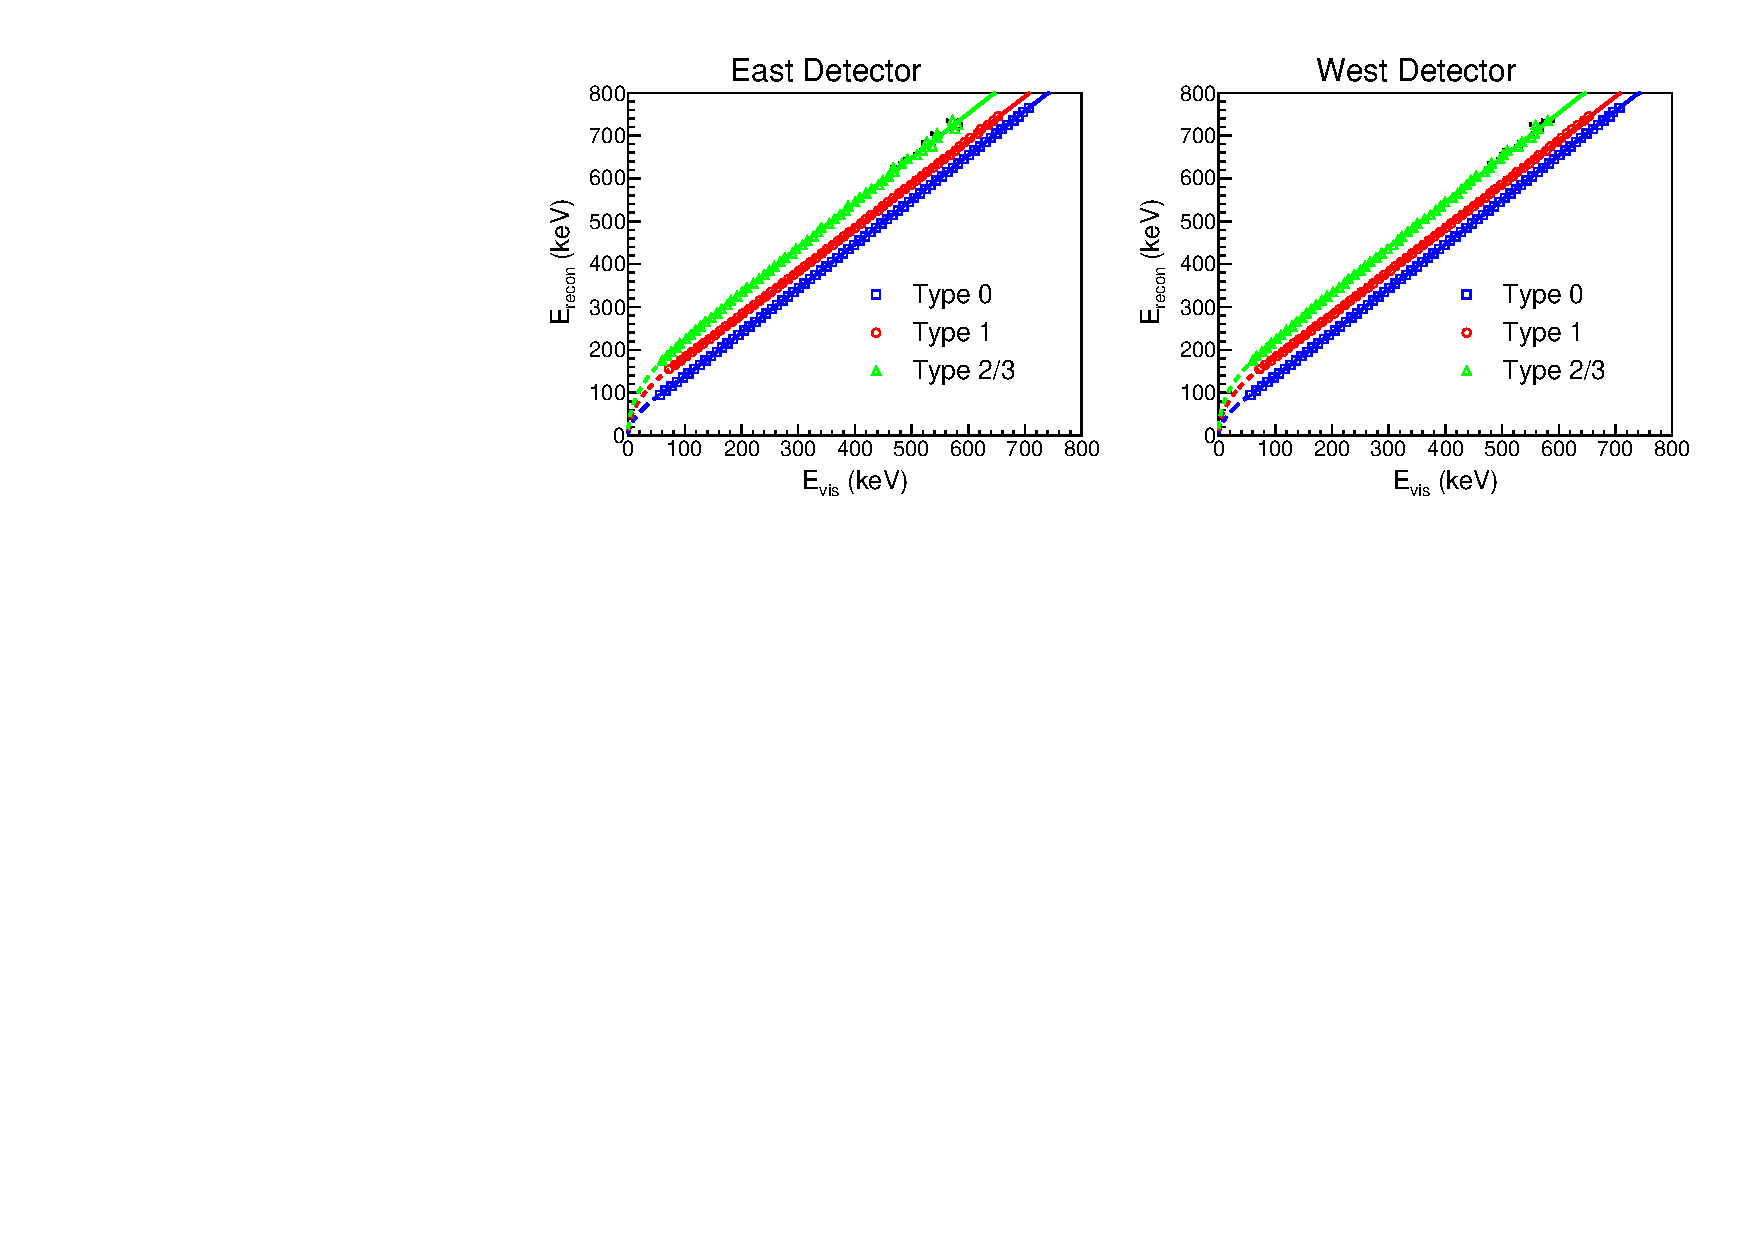
\includegraphics[scale=0.78]{3-UCNAAnalysis/2011-2012_Evis_to_Erecon.pdf}
  \caption{Parameterization between $E_{\mathrm{vis}}$ and $E_{\mathrm{recon}}$ for
    2011-2012. The mapping for the other geometries are very similar and thus are
    not shown.}
  \label{fig:Erecon}
\end{figure}

The mapping between $E_{\mathrm{vis}}$ and $E_{\mathrm{recon}}$ is determined separately
for 2011-2012, 2012-2013, and 2012-2013 with isobutane in the wirechamber.
Using the simulated $\beta$-decay spectrum and a characteristic set of detector
response variables, the simulated events are processed in the same manner as
they would be for data. They are identified as Type 0, 1, or 2/3, and their
$E_{\mathrm{vis}}$ values for each detector are determined. Then the events are
grouped into histograms using their initial energy (we will call it $E_{\mathrm{recon}}$,
but really this is the true energy of the events), with the histogram bins corresponding
to 10~keV groups from 0~keV to 790~keV. Then each of these histograms are fit to
determine the average $E_{\mathrm{vis}}$ value for a given $E_{\mathrm{recon}}$. The results
of these fits for each event type in each detector for 2011-2012 is shown as the data
points in Figure \ref{fig:Erecon}. The other geometries look very similar and thus are
left out. Data points with low statistics at low energies were dropped.

The fit to the data is of the form
\begin{equation}
  E_{\mathrm{recon}} = C_1 + C_2E_{\mathrm{vis}} + \frac{C_3}{E_{\mathrm{vis}}} + \frac{C_4}{{E_{\mathrm{vis}}}^2},
\end{equation}
and then the fit is extrapolated continuously to zero from the lowest energy data point using
\begin{equation}
  E_{\mathrm{recon}} = C_5{E_{\mathrm{vis}}}^{C_6}
\end{equation}
with the parameters $C_5$ and $C_6$ determined by ensuring the two equations are equal at the
transition point along with their first derivatives.

Using the fitted parameters, an $E_{\mathrm{recon}}$ value is determined
for every event by plugging its weighted average $E_{\mathrm{vis}}$ into the proper equation.
It should be noted that for Type 1 events, the visible energies of both the East and West
detectors are added together when determining the parameterization, so
the same is done when applying the above parameterization to data. This is done to utilize as much
detector information as possible. The side for a Type 1 event is set to
the detector with the earlier trigger, making it the primary detector.
Thus, for a Type 1
event, one would plug $E_{\mathrm{vis}} = E_{\mathrm{vis}}^E + E_{\mathrm{vis}}^W$ into the $E_{\mathrm{recon}}$
equation for the side that triggered first.

\section{Detector Response Model} \label{sec:DetectorResponseModel}
The goal of the Detector Response Model is to create an estimate of the potential PMT
signals from the $E_Q$ produced in the simulation. While it is true that the simulation
captures the true physics of the experiment, the simulation output does not properly
represent the data signals.
For instance, the purely simulated scintillator energy depositions have sharp peaks at the
maximum allowed energy deposition with low
energy tails, a result of energy losses elsewhere in the apparatus. The less probable outer shell
conversion electron lines are also visible in the simulation. The data signals
on the other hand are smeared out in a Gaussian fashion, with no possible
resolution of the outer shell electron lines.
The Gaussian-like peaks arise from finite resolution effects and
must be incorporated in the simulatin using parameters calculated
from real data.  


\subsection{Extracting simulated ADC values}


Recall from Section \ref{sec:EnergyResponse} that we can relate a PMT signal,
$\mathrm{ADC}_i$, to the energy deposited in the scintillator
using Equation \ref{eq:EvisResponse}.
Our goal is to reverse engineer this expression to write an ADC signal as a
function of the visible energy, noting that the visible energy is directly
related to the quenched energy from simulation. Directly from \ref{eq:EvisResponse}
we can trvially write down:
%
\begin{equation} \label{eq:pmtResponse}
\mathrm{ADC}_i = f_i^{-1}\big(\eta_i(x,y) E_{\mathrm{vis},i} \big)/g_i + p_i
\end{equation}
%
where we have dropped the time dependence for brevity. For the time being, take
the PMT response functions $f$ and the position dependent response values $\eta_i(x,y)$ to be known,
as their determination is addressed in Sections \ref{ssec:linCurves} and \ref{sssec:posmaps}
respectively.

Now we can further generalize this expression by recalling that the gain and the pedestals
were extracted from distributions, with the values used in the gain correction and pedestal
subtraction equal to the mean of the distribution. Technically speaking though, there is a
well-defined probability that the actual gain and pedestal were not equal to this mean, but rather
sampled some other value from the distributions. To account for this, we will add a spread
to the gain and pedestal:
%
\begin{equation} 
  \mathrm{ADC}_i = f_i^{-1}\big(\eta_i(x,y)  E_{\mathrm{vis},i} \big)/\big(g_i\pm\delta g_i\big) + \big(p_i \pm \delta p_i\big).
  \label{eq:pmtResponse}
\end{equation}
%
This is to be interpreted as the pedestal (gain) being sampled from a normal
distribution with mean $p_i$ ($g_i$) and sigma $\delta p_i$ ($\delta g_i$).

Remember the goal is to plug in $E_Q$ and return an ADC value for each PMT, so we must next
relate $E_Q$ to $E_{\mathrm{vis}}$. What we really need is an expression for $\eta_iE_{\mathrm{vis}}$ in terms of $E_Q$.
Backtracking for a moment, we recall that $E_{\mathrm{vis}}$ is by definition the result
of plugging the ADC response into equation \ref{eq:EvisResponse}. The ADC response is proportional to the final amount of charge
that reaches the anode in a PMT, and is thus the product
of several stochastic processes and is only an estimate of the initial light from the scintillator that reached
the photocathode. In fact, every dynode within the photomultiplier introduces stochasticity into the process, as every time an electron
strikes a dynode, the number of emitted electrons is Poisson distributed. The final number of electrons that reach the anode
can be expressed as several nested Poisson distributions,
with the initial number of events equal to the number of photoelectrons present at the photocathode. The series of Poisson
processes randomizes the final number of electrons seen by the anode, and therefore randomizes the ADC response.

Let us attempt to estimate the total number of electrons that reach the anode, which in turn yields something
proportional to the ADC response and thus also related to $E_{\mathrm{vis}}$. We will use only two nested Poisson
processes, where the first emulates the gain from the very first dynode, and the second captures the gain from the rest of
the dynodes as a whole. We then have:
%
\begin{equation}
  N_i^{\mathrm{tot}} \approx \mathrm{Pois}(g_r \cdot \mathrm{Pois}(g_d \cdot N_i)),
  \label{eq:ntot1}
\end{equation}
%
where $N_i^{\mathrm{tot}}$ is the total number of electrons to reach the PMT anode, $g_d$ is the gain of the first dynode,
$g_r$ is the total gain of the rest of the dynodes, and $N_i$ is the number of initial photoelectrons at the photocathode.
This number of photoelectrons is precisely related to the amount of light which reaches the PMT, which as a matter of fact
we defined as $N_i = \alpha_i \eta_i(x,y) E_Q$ in Section \ref{ssec:combinePMT}. Here $\alpha_i$ is again the PMT resolution
factor which relates the number of photoelectrons to energy, and for now we should take it as known (see Section
\ref{ssec:PMTresolution}).

Rewriting Equation \ref{eq:ntot1} we have
\begin{equation}
  N_i^{\mathrm{tot}} \approx \mathrm{Pois}(g_r \cdot \mathrm{Pois}(g_d \cdot \alpha_i \eta_i(x,y) E_Q)).
  \label{eq:ntot2}
\end{equation}
Here $N_i^{\mathrm{tot}}$ is an estimate of the total number of electrons that reach the PMT anode, but we can turn it
into an estimate of the number of initial photoelectrons simply by dividing by each of the dynode gain factors:
\begin{equation}
  \overline{N_i} \approx \frac{1}{g_rg_d}\mathrm{Pois}(g_r \cdot \mathrm{Pois}(g_d \cdot \alpha_i \eta_i(x,y) E_Q)).
  \label{eq:ntot3}
\end{equation}

But now we should realize that we already have an expression for $\overline{N_i}$ from Section \ref{ssec:combinePMT}, namely
\begin{align}
  \overline{N_i} &= N_i \pm \sqrt{N_i} \\
  &= \alpha_i \eta_i(x,y) E_Q \pm \sqrt{\alpha_i \eta_i(x,y) E_Q} \\
  &= \alpha_i \eta_i(x,y) \Bigg( E_Q \pm \sqrt{\frac{E_Q}{\alpha_i \eta_i(x,y)}}\Bigg) \\
  &= \alpha_i \eta_i(x,y) E_{\mathrm{vis},i} 
  \label{eq:bam}
\end{align}
where we used Equation \ref{eq:Evisi} in the last line. Thus we can now write
\begin{equation}
   \alpha_i \eta_i(x,y) E_{\mathrm{vis},i} \approx \frac{1}{g_rg_d}\mathrm{Pois}(g_r \cdot \mathrm{Pois}(g_d \cdot \alpha_i \eta_i(x,y) E_Q)),
  \label{eq:ntot4}
\end{equation}
directly from which our desired expression for $\eta_i(x,y) E_{\mathrm{vis},i}$ follows:
\begin{equation}
   \eta_i(x,y) E_{\mathrm{vis},i} \approx \frac{1}{\alpha_i g_rg_d}\mathrm{Pois}(g_r \cdot \mathrm{Pois}(g_d \cdot \alpha_i \eta_i(x,y) E_Q)).
  \label{eq:etaEvis}
\end{equation}

The last outstanding question is then what values to use for the gain of the dynodes. The PMTs are
Hamamatsu model R7725, run typically between 1100-1300~V. From the Hamamatsu documentation \cite{hamamatsu},
this model PMT has a total gain of $\sim2\times 10^5$ when run at $\sim1100$~V. Since this PMT has 12 stages (dynodes),
if we assumed equal gain on every dynode this would give $g_d\approx2.7$. But the first dynode is biased $4\times$ higher
than the rest, so it should exhibit a higher gain. Thus the gain of the first dynode was set to $g_d=16$, which then determines
that the gain of the rest of the dynodes combined should be $g_r = 2\times 10^5/g_d = 12500$.

\subsection{Applying the Detector Response Model}

With Equation \ref{eq:etaEvis} to approximate $\eta_i(x,y) E_{\mathrm{vis},i}$ for each PMT, this can be plugged into
$f^{-1}$ to return an initial ADC estimate in the form of Equation \ref{eq:pmtResponse}. The gain and pedestal
widths could be taken as zero without substantial loss of model integrity, as the majority of the detector
response has been captured using the position dependent response, PMT resolution factors, and sampling of the
Poisson processes. The gain is stable enough that including a sampling of the width introduces $<1\%$ fluctuations
in modeled ADC, and so it was ignored. The pedestal distributions for each PMT were sampled and used in the
Detector Response Model, as this gives a width to a signal with no energy deposition as is seen in the data.
To apply the random sampling of the pedestal, a Gaussian is randomly sampled with mean equal to zero and sigma equal
to the rms recorded for that PMT in the run of interest. This random value is then added to the ADC estimate. 

Once all $\mathrm{ADC}_i$ have been calculated, the two-fold trigger model must be applied.
The PMT trigger thresholds as determined in Section \ref{sec:triggerThresh} are retrieved for the run of interest.
The probability of triggering is read from the trigger threshold function for an individual PMT, and then
acceptance/rejection is performed to decide whether the PMT triggered. The basic two-fold trigger logic is
applied, so if two or more PMTs trigger, the scintillator on that side is recorded as having a two-fold trigger.

With the modeled $\mathrm{ADC}_i$ values calculated and the pedestal width sampled and added to the signal, the ADC values
are treated as though they are data and plugged into Equation \ref{eq:EvisResponse}. This subtracts the mean pedestal,
applies the gain correction, and then maps the ADC response back to a new estimate of $\eta_i(x,y) E_{\mathrm{vis},i}$
using the calibration linearity curve $f(\mathrm{ADC})$. Upon dividing by the position dependent light transport
value $\eta_i(x,y)$, one has estimates for the visible from all PMTs.

At this point, the individual $E_{\mathrm{vis},i}$ are combined using the now familiar methods of Section \ref{ssec:combinePMT}.
Then a final $E_{\mathrm{recon}}$ value is determined via the normal parameterization. Everything about the simulation event
now resembles a data event, and thus the analysis procedure for data and simulation becomes identical.




%---------------------------------------------------------------------------------------


\section{Calibration Overview}

In the next chapter, we will take an in depth look at the calibrations of both
the wirechamber and the scintillator. Here we simply highlight their use in the analysis.

\subsection{PMT Calibration} \label{ssec:PMTCal}

The PMT calibration, as mentioned in Section \ref{sssec:scintEnCal},
uses well known conversion electron sources
to understand the detector response to there well-defined energies. By comparing the detector
response (coupling both ADC values and position map values) to simulated responses,
we can map ADC signals from each PMT to visible energies deposited
in the scintillator. These calibrations parameterize the detector response so that the
functional form of the calibration can be applied to the $\beta$-decay data.

\subsection{Wirechamber Calibration}

The wirechamber calibration relates the anode signal in the MWPC to an energy deposited in the MWPC. This is
primarily useful for separating the Type 2/3 backscattering events, as the
energy deposition in the MWPC is not used within the reconstruction of an electron's initial
energy. This separation is important though as it drastically reduces the systematic
correction for these backscattering events.
 

\section{Polarimetry} \label{sec:polarimetry}

The polarimatry analysis was carried out Eric Dees of North Carolina State University and
deserves the attention of an entire dissertation itself. The previous polarimetry measurement
is described in detail in a dissertation by Adam Holley \cite{holley2012ultracold}. A major
difference between the previous depolarization measurement and the current depolarization
hinges upon the installation of the shutter between the spin flipper and decay trap. An
update of the new polarimetry measurement method can be found in the publication of the result
presented within this dissertation \cite{brown2017}.

\begin{figure}[h] 
\centering
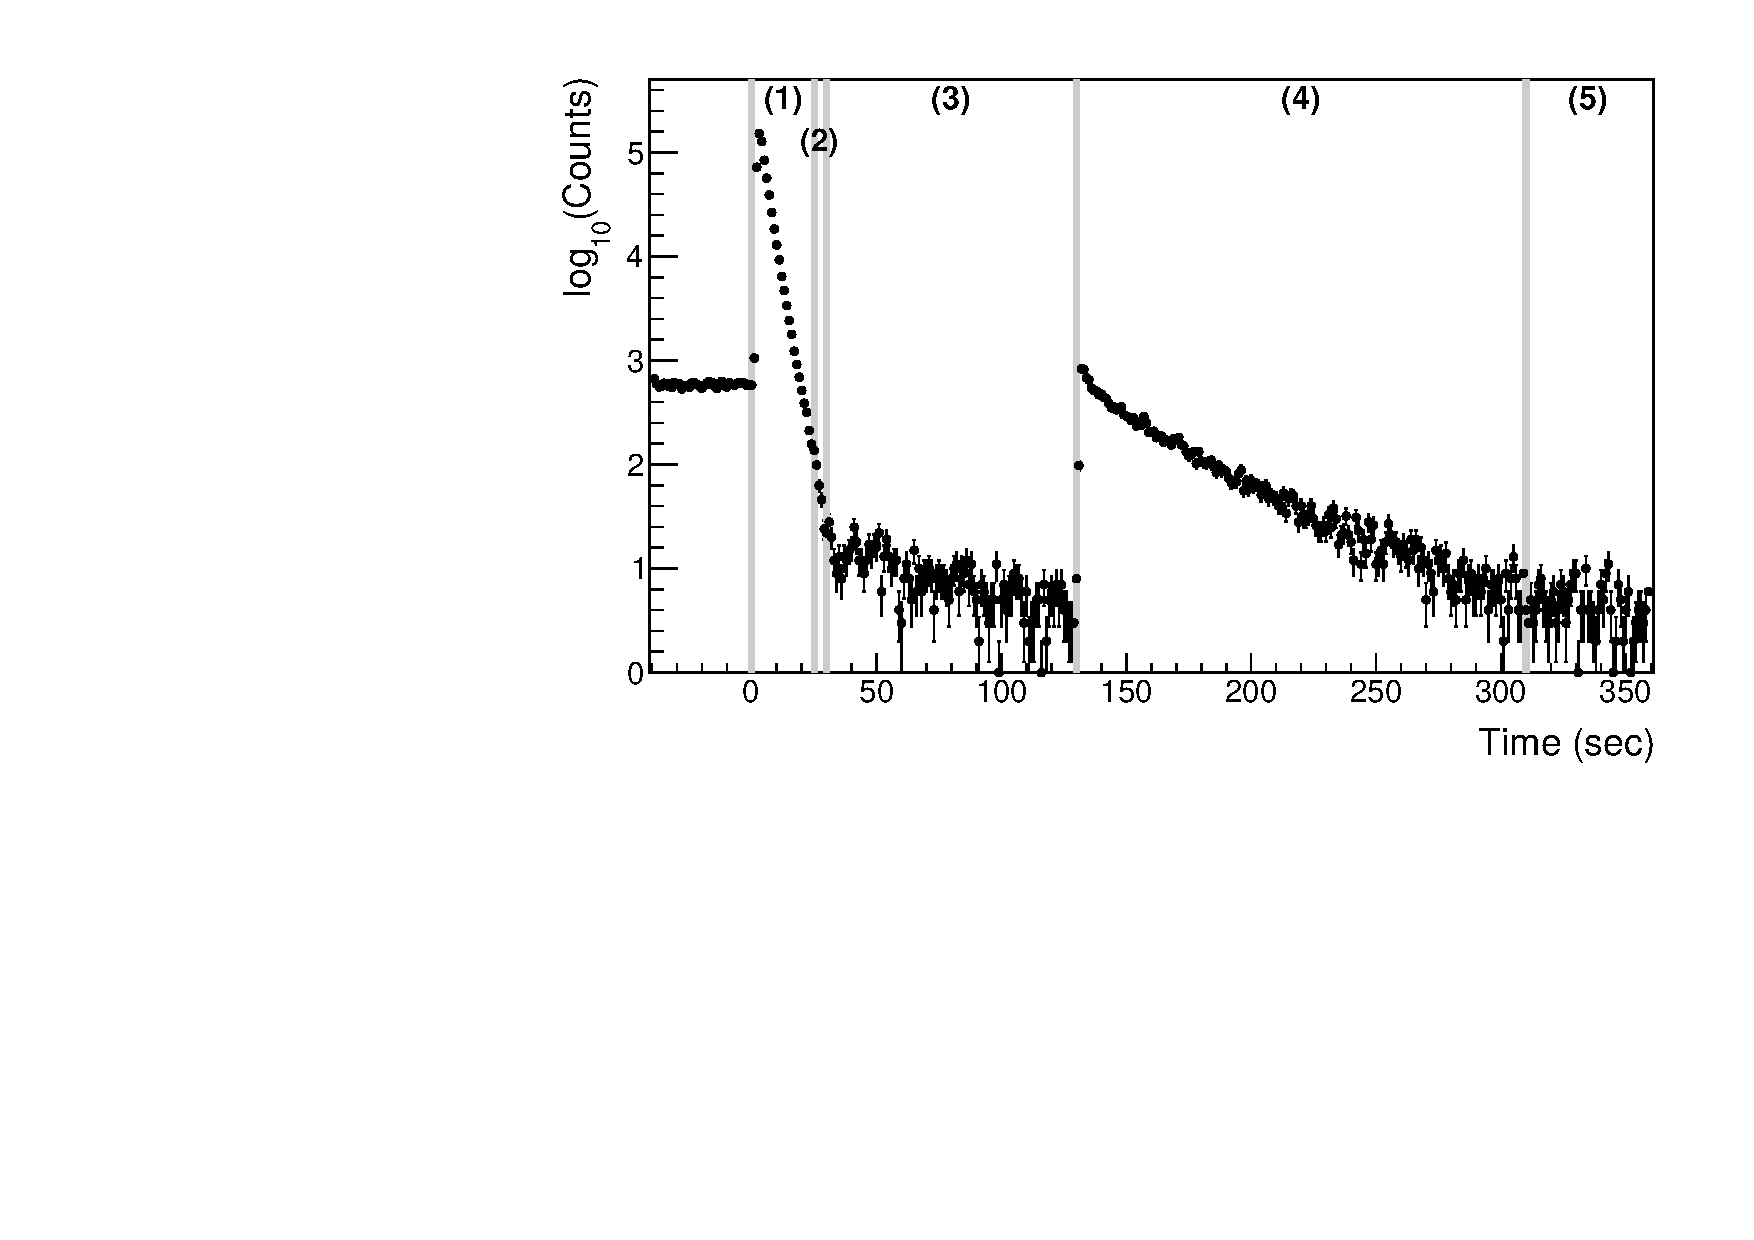
\includegraphics[scale=.55]{3-UCNAAnalysis/Switcher_signals.pdf}
\caption{Figure courtesy of E. Dees and A. R. Young as published in \cite{brown2017}.
  ``Switcher signal as a function of time, during ``D''-type runs: (1) the shutter
  closes and the switcher state changes, permitting UCN in the
  guide outside the decay volume to drain to the switcher UCN detector, (2) the AFP
  spin-flipper changes state, allowing depolarized neutrons in the guides outside the
  decay volume to drain to the switcher, (3) the shutter opens, permitting depolarized
  neutrons within the decay volume to drain to the switcher detector, (4) the AFP
  spin-flipper returns to its initial state, allowing the initially loaded spin state
  to drain from the decay volume, (5) backgrounds are measured after the UCN
  population in the decay volume has drained away.  The presented data were taken in 2011
  and UCN loaded into the decay volume with the spin-flipper off.''}
\label{fig:switcherSignal}
\end{figure}

Here is a brief description of the polarimetry measurement.
The polarimetry measurement determines the average neutron polarization in each spin state using
the depolarization runs that follow every $\beta$-decay run. As detailed in section
\ref{sec:polarization}, the neutrons are initially polarized by traversing the 7~T primary
polarizing magnet, and then the desired spin is chosen using the AFP spin flipper.

After a $\beta$-decay run, the depolarization run begins by closing the shutter and changing the switcher
state to allow
the UCN to flow into the switcher detector for measurement of UCN populations. The switcher signal
as a function of time can be found in Figure \ref{fig:switcherSignal}. The guides are cleaned of UCN while
the UCN population in the trap remains contained. Then the spin flipper state is changed allowing the
neutrons that were trapped between the 7~T magnet and the decay trap to pass back through the high
field region (these trapped neutrons result from UCN who underwent an unwanted spin flip after passing
the high field region, subsequently keeping them passing the 7~T field). Now that the guides are cleaned,
the shutter is opened and all UCN with spins not equal to the desired loaded spin are emptied (remember that
the spin flipper is switched from its original state). Once this population has been measured in the
switcher detector, the spin-flipper state is again changed back to its original state, and the
properly polarized UCN population is measured in the switcher detector. This process is followed by a short
background measurement in the switcher detector.

The ratio of these populations is then extrapolated back to the equilibrium population as established
during $\beta$-decay running by utilizing further \textit{ex situ} measurements and comparisons with
simulation. The results of these measurements as well as the correction to the uncertainty resulting
from imperfect polarization ($P<1$) can be found in Section \ref{ssec:polCorr}.






\copyrightnotice


% Chapter 4
\chapter{UCNA Analysis}
\label{ch:UCNA_Analysis}
%%%%%%%%%%%%%%%%%%%%%%%%%%%%%%%%%%%%%%%%%%%%%%%%%%%%%%%%%%%%%%%%%%%%%%%%%%%%%%%
%%%%%%%%%%%%%%%%%%%%%%%%%%%%%%%%%%%%%%%%%%%%%%%%%%%%%%%%%%%%%%%%%%%%%%%%%%%%%%%
%%%%%%%%%%%%%%%%%%%%%%%%%%%%%%%%%%%%%%%%%%%%%%%%%%%%%%%%%%%%%%%%%%%%%%%%%%%%%%%

Detector calibrations are a beautiful combination
of simulation and data manipulation which allows one to extract the energy of
an event based solely on some electronic signal. Imagine a baseball pitcher
throwing a fastball into a sheet, and the observer behind the sheet must
determine the velocity of the ball from only seeing the impression the pitch
made on the sheet. This is the task every nuclear physics experiment is faced
with, only the baseball is a particle and the sheet is our detecotr system.
Below we focus on the energy calibration of our apparatus.

%--------------------------------------------------------------

\section{Simulation}
\label{sec:Simulation}

The simulations and application of the
detector response model provide a suitable starting
point for discussing the analysis, as the calibration of the data hinges
strongly on the simulation results. There is a notable dependence of the
response model which depends on data, but this will be addressed as needed
when describing the calibration.

The simulation work for this thesis was completed
using the Geant4 simulation software package. The geometry of the
apparatus was duplicated
to the best precision possible and benchmarked against data after
the detector response model was applied. The structure
of the simulation code did not change from those in the previous analysis
as described in \cite{mpmThesis}, although minor changes were
made to the geometry to reflect real adjustments to the experimental
apparatus.

\subsection{Input}
\subsubsection{Conversion Electron Sources}
make sure to show figures or a table with the conversion lines
\subsubsection{Activated Xenon}
\subsubsection{$\beta$-decay Electrons}

\subsection{Output}
The Geant4 simulation provides adequate trajectory tracking along with
the energy deposition along these tracks. Obviously we have access to far
more information in the simulation than we do with actual data, so the first
task is to construct observables related to those coming from the detectors.

\subsubsection{Energy Deposition}
By tallying the energy deposited along an entire track within some subset
of the geometry, one can reconstruct the energy deposited anywhere within
the SCS. The areas of highest interest for the sake of analysis are the
wirechambers and the scintillators. The energy deposited in the scintillator
is of utmost importance, as the analysis can be completed without knowledge
of the energy deposition in the wirechamber, where determination of energy
deposition is only used for type II/III separation. From here on,
the energy lost in the scintillator, as determined from simulation, will be
referred to as $E_{dep}$. This is the maximum energy which could be detectable
for an event in the data if no inconspicuous energy losses existed.

\subsubsection{Quenched Energy}
Show Birk's law. Talk about MPM and jianglai's analysis to determine
quenching parameters. Then talk about the modification using BradF's note
and show the shift to the functional form. Also show a figure which shows
the quenched energy vs Edep.

\subsubsection{Position of Detector hits}
Talk briefly of importance of position dependence, and maybe address
the way the position for the wirechamber and scintillator are calculated.
I believe this was a weighted average of the track positions where the
weights are given by the energy deposition.

\subsection{Simulating Detector Response}
While all pertinent components of the experimental apparatus were included
in the simulation, the detector response is not inherent within our
output. You may notice from (figure with quenched energy) that this
doesn't resemble the gaussian peaks normally seen in a detector signal.
The gaussian-like peaks arise from finite resolution effects and
must be put in defacto using parameters calculated
from real data. The better we understand the conversion from a pure simulation
energy output to a response which mimics that from our actual detectors, the
more credence we can put in our calibration.For the time being, the model will be introduced with parameter determination addressed as it arises. 

\subsubsection{Application of the PMT Response Model}

Recall from section \ref{sssec:pmtModel} that we can relate a digital signal
in a PMT, $ADC_i$, to it's light output using Equation \ref{eq:pmtResponse}.
By reverse engineering this process, we can use a purely simulated $E_Q$ and
simulate an ADC channel, so that we can process the simulated data in
exactly the same way we process real data.



\subsubsection{$E_{true}$ reconstruction}
%----------------------------------------------------------

\subsection{Wirechamber Calibration}

Blah Blah

%----------------------------------------------------------

\section{Energy Calibration}
\subsection{Electron Conversion Sources}
\subsection{Linearity Curves}
\subsection{PMT Resolution}









\copyrightnotice

% Chapter 5
\chapter{UCNA Results}
\label{ch:UCNA_Results}
%%%%%%%%%%%%%%%%%%%%%%%%%%%%%%%%%%%%%%%%%%%%%%%%%%%%%%%%%%%%%%%%%%%%%%%%%%%%%%%
%%%%%%%%%%%%%%%%%%%%%%%%%%%%%%%%%%%%%%%%%%%%%%%%%%%%%%%%%%%%%%%%%%%%%%%%%%%%%%%
%%%%%%%%%%%%%%%%%%%%%%%%%%%%%%%%%%%%%%%%%%%%%%%%%%%%%%%%%%%%%%%%%%%%%%%%%%%%%%%


\section{Constructing an Asymmetry} \label{sec:asymmetry}

\subsection{Decay Rate Model}
As discussed in earlier in section \ref{ssec:neutronAsymmParam},
the nominal decay rate for polarized neutrons with no detection of
final-state spins is expressed in terms of the spin
vector of the neutron and all possible correlations to the products \cite{jackson1957a}.
For simplicity,
we begin by writing the differential decay rate for the case where only the electron
momentum is detectable (and assuming no BSM terms): 
%
\begin{equation} \label{eq:simpleRate}
\Gamma\left(E,\Omega\right)=C \cdot S(E) \cdot \big( 1+A(E)\beta\cos\theta \big),
\end{equation}
%
\noindent where $S(E)$ is the Standard Model differential decay rate for unpolarized
$\beta$-decay, $C$
is a constant which encompasses anything not included in $S(E)$ and serves the 
purpose of absorbing other constants, $A(E)$ is the 
energy dependent electron asymmetry parameter, $\beta\equiv v/c$ is the electron
velocity, and 
$\theta$ is the angle between the spin of the neutron and the electron momentum.

We can also introduce an average polarization of the neutrons, giving
%
\begin{equation}
  \Gamma\left(E,\Omega\right)=C \cdot S(E) \cdot \epsilon \cdot
  \big( 1+ \langle P \rangle\cdot A(E)\beta\cos\theta \big),
\end{equation}
%
\noindent where $\epsilon$ is the loading efficiency of neutrons
in this spin state which I haven't absorbed
into the constant for reasons to be seen, and 
$\langle P \rangle$ is the polarization, i.e. a number between 0 and 1 (very close to 1
in our case).

At this point, assumptions can be made regarding the experimental setup utilized
to further express the decay rate in terms of detector rates. Due to the spins
being aligned with the 1 T magnetic field in the decay trap, electrons emitted with
a momentum component along the spin will spiral towards one detector, while electrons
with a component of momentum opposite the spin will be detected in the opposite 
detector. If we fix the $z$-axis using the static position of our
apparatus, we can call the detector at $\theta=0$ detector
1 and the opposite detector 2. 

Now, all electrons with $0 < \theta < \pi/2$ will head towards detector 1 and those 
with $\pi/2 < \theta < \pi$ will be directed towards detector 2. The solid angle can
then be integrated out for each detector by integrating $\phi$ from $(0,2\pi)$ and
$\cos\theta$ over the intervals given, where the integral of $\cos\theta$ over detectors
1 and 2 yields $+1/2$ and $-1/2$ respectively: 
%
\begin{equation} 
  \Gamma_{1,2}\left(E\right)= 2\pi \cdot C \cdot S(E) \cdot
  \epsilon \cdot \eta_{1,2}(E) \left[ 1+ \langle P \rangle\cdot A(E)\beta
    \left(\pm_{1,2}\frac{1}{2}\right) \right],
\end{equation} 
%
\begin{equation} 
  \Gamma_{1,2}\left(E\right)=C' \cdot S(E) \cdot \epsilon \cdot \eta_{1,2}(E)
  \left[ 1 \pm_{1,2} \langle P \rangle\cdot A(E) \frac{\beta}{2} \right],
\end{equation} 
%
\noindent with $\eta_{1,2}(E)$ signifying energy dependent electron
detection efficiencies for detectors 1 and 2. 

Thus far we have assumed a fixed polarization, but in UCNA we have the ability to 
flip the spin of the neutrons prior to loading. We call these states flipper on ($+$) 
and flipper off ($-$), denoted by $\langle P \rangle_{\pm}$. The flipper on state introduces a
negative in front of the polarization efficiency
due to the fact that the spin $\vec{\sigma}$ is now aligned with $-\hat{z}$, thus reversing the sign
of $\vec{\sigma}\cdot\vec{p_{e}}$ with respect to the prior assumption of $\vec{\sigma}$ in $+\hat{z}$:
%
\begin{equation}
  \Gamma_{1,2}^{\pm}\left(E\right)=C' \cdot S(E) \cdot \epsilon_{\pm} \cdot \eta_{1,2}
  \left[ 1 \pm_{1,2} 
\left(\mp \langle P \rangle_{\pm}\right) \cdot A(E) \frac{\beta}{2} \right],
\end{equation} 
%
\noindent where $\epsilon_{\pm}$ accounts for differing loading efficiencies for 
different spin states.

If we now assume that we are equally as efficient at polarizing in either spin state, we
can say $\langle P \rangle_{+}=\langle P \rangle_{-}=\langle P \rangle$
(extraction of the asymmetry under the super-ratio technique not assuming this
condition can be found later in Section \ref{ssec:polSep}) giving:
%
\begin{equation} \label{eq:decayRate}
  \Gamma_{1,2}^{\pm}\left(E\right)=C' \cdot S(E) \cdot \epsilon_{\pm} \cdot \eta_{1,2}
  \left[ 1 \pm_{1,2} 
    \left(\mp \langle P \rangle \right) \cdot A(E) \frac{\beta}{2} \right].
\end{equation}
%

\subsection{Super-Ratio}

A simple asymmetry over some energy bin for a single 
polarization state can be defined as
%
\begin{equation} 
A_{\mathrm{simple}} = \frac{\Gamma_1 - \Gamma_2}{\Gamma_1 + \Gamma_2}, 
\end{equation}
%
\noindent and assuming that the efficiencies $\eta_1$ and $\eta_2$ are the same one
finds
%
\begin{equation} \label{eq:Asimple}
A_{\mathrm{simple}} = \langle P \rangle \cdot A(E) \cdot \frac{\beta}{2},
\end{equation}
%
\noindent where $\beta$ is calculated as either the velocity associated with the energy 
at the center of the bin or the average energy of the bin. The distinction is
unimportant as this is later corrected for as part of the angular acceptance correction
detailed in Section \ref{sssec:cosThetaCorr}.

In reality we cannot assume with certainty that the detectors are identical, but we can 
utilize the fact that we can flip the spins to cancel differing efficiencies. If we 
take two runs with opposite polarizations, we can define the super-ratio asymmetry in 
some energy range as:
%
\begin{equation} \label{eq:A_SR_frac}
A_{\mathrm{SR}} = \frac{1-\sqrt{R}}{1+\sqrt{R}} ,
\end{equation}
\noindent where 
\begin{equation} \label{eq:R}
 R = \frac{\Gamma_{1}^+ \cdot \Gamma_{2}^-}{\Gamma_{1}^- \cdot \Gamma_{2}^+}.
\end{equation}

Some algebra yields an identical expression to Equation \ref{eq:Asimple},
%
\begin{equation*}
R = \frac{ \left[ C'  S(E)  \epsilon_{+}  \eta_{1} \left[ 1 + 
      \left(- \langle P \rangle \right)  A(E) \frac{\beta}{2} \right] \right] 
\left[ C'  S(E)  \epsilon_{-}  \eta_{2} \left[ 1 - 
    \left(+ \langle P \rangle \right)  A(E) \frac{\beta}{2} \right] \right] }
{ \left[ C'  S(E)  \epsilon_{-}  \eta_{1} \left[ 1 + 
      \left(+ \langle P \rangle \right)  A(E) \frac{\beta}{2} \right] \right] 
\left[ C'  S(E)  \epsilon_{+}  \eta_{2} \left[ 1 - 
    \left(- \langle P \rangle \right)  A(E) \frac{\beta}{2} \right] \right] },
\end{equation*}
%
\begin{equation*}
R = \frac{ \left[ 1 + \left(- \langle P \rangle \right)  A(E) \frac{\beta}{2} \right] 
\left[ 1 - \left(+ \langle P \rangle \right)  A(E) \frac{\beta}{2} \right]  }
{  \left[ 1 +  \left(+ \langle P \rangle \right)  A(E) \frac{\beta}{2}  \right] 
 \left[ 1 -  \left(- \langle P \rangle \right)  A(E) \frac{\beta}{2} \right]},
\end{equation*}
%
\begin{equation*}
R = \frac{ \left[ 1 -  \langle P \rangle  A(E) \frac{\beta}{2} \right]^2 }
{  \left[ 1 + \langle P \rangle  A(E) \frac{\beta}{2}  \right]^2 },
\end{equation*}
%
\noindent and plugging into $A_{\mathrm{SR}}$
%
\begin{equation*}
  A_{\mathrm{SR}} = \frac{1-\frac{ \left[ 1 -  \langle P \rangle  A(E) \frac{\beta}{2} \right] }
{  \left[ 1 + \langle P \rangle  A(E) \frac{\beta}{2}  \right] } }
  {1+\frac{ \left[ 1 -  \langle P \rangle  A(E) \frac{\beta}{2} \right] }
{  \left[ 1 + \langle P \rangle  A(E) \frac{\beta}{2}  \right] }},
\end{equation*}
%
\begin{equation*}
A_{\mathrm{SR}} = \frac{2 \langle P \rangle A(E) \frac{\beta}{2}}{2},
\end{equation*}
%
\begin{equation} \label{eq:A_SR}
A_{\mathrm{SR}} = \langle P \rangle A(E) \frac{\beta}{2}.
\end{equation}

The super-ratio not only cancels the detector efficiencies, but any difference between the
integrated rates between the two spin states also cancel.

\subsection{Extracting $A_0$}

The quantity of interest is not the raw measured asymmetry, or even $A(E)$,
but rather $A_0$, which is directly proportional to $\lambda=g_A/g_V$, yielding a direct 
measurement of the axial vector coupling constant if the CVC hypothesis is assumed. 

$A_0$ manifests itself in our measured asymmetry as:
%
\begin{equation}
A_0 = A(E) \cdot \left( 1 + \Delta(E) \right),
\end{equation}
%
\noindent where $\Delta(E)$ is the energy dependent correction to the measured asymmetry
from theory corrections and experimental systematic effects, all of which will be
described in detail in \ref{sec:systematics}. The modifications from theory were
also mentioned in chapter 1.

Solving \ref{eq:A_SR} for $A(E)$ and inserting into the above expression, we have 
%
\begin{equation}
  A_0 = \frac{\big( 1 + \Delta(E) \big) \cdot A_{\mathrm{SR}}(E) }
  {\langle P \rangle \cdot \beta/2},
  \label{eq:A0}
\end{equation}
%
\noindent where again $\beta=v/c$. 

With an energy dependent expression for $A_0$, we can bin our data in discrete
energy bins, evaluate $\beta$ at the midpoint of the bin, apply appropriate energy
dependent corrections, and then fit the resulting collection of $A_0$ values with a
constant. Careful selection of the energy range to fit over is discussed
in \ref{ssec:enRange}. 


%--------------------------------------------------------------------------------------------------
\section{Systematic Corrections and Uncertainties} \label{sec:systematics}

Measuring any quantity without imparting a systematic shift in the result due to
imperfect experimental techniques is nearly impossible; but what is more dangerous
to the result is not understanding these shifts. This section discusses how well
we understand the theoretical and experimental effects present in the UCNA
experiment that cause us to measure an asymmetry that is not directly equal to
the parameter of interest, thus requiring corrections.

\subsection{Definition of $\Delta$}

We adopt a similar formalism for systematic corrections as previously defined in
\cite{mpmThesis}, at least as far as the definition of the correction is concerned.
If we have an asymmetry $A(E)$ measured without some correction $i$,
then we can define $A'(E)$ as
%
\begin{equation} \label{eq:aprimedelta}
  A'(E) = \big( 1 + \Delta_i(E) \big) \cdot A(E),
\end{equation}
%
\noindent where $A'(E)$ is the new corrected asymmetry with systematic effect $i$ removed.
Rearrangement of the above equation provides a definition for $\Delta_i$:
%
\begin{equation} \label{eq:delta}
  \Delta_i(E) = \frac{A'(E)}{A(E)} - 1
\end{equation}
%
This is useful as most corrections are determined by studying the effect on the asymmetry
from some aspect of the experiment via Monte Carlo, so energy dependent corrections can
be constructed and applied to data.

If the uncertainty on correction $\delta\Delta_i$, denoted $\delta \Delta_i$,
has been determined, we can also define
the uncertainty on the resulting asymmetry $\delta A'(E)$ via normal error propagation
techniques as
%
\begin{equation} 
  \delta A'(E) = A(E) \cdot \delta\Delta_i(E),
\end{equation}
%
\begin{equation} 
  \frac{\delta A'(E)}{A'(E)} =  \frac{ \delta\Delta_i(E)}{1+\Delta_i(E)}.
\end{equation}

Now the collection of all corrections, if extracted independently, will commute, and thus
provides
%
\begin{equation}
1+\Delta(E)=\big(1+\Delta_1(E)\big)\big(1+\Delta_2(E)\big)\big(1+\Delta_3(E)\big)\ldots,
\end{equation}
%
\noindent such that a final corrected asymmetry $A'''^{\ldots}$ can be written as 
%
\begin{equation*}
A'''^{\ldots}(E) = \big(1+\Delta(E)\big) \cdot A(E),
\end{equation*}
%
\begin{equation}
A'''^{\ldots}(E) = \Big(\prod_i\big(1+\Delta_i(E)\big)\Big)\cdot A(E).
\end{equation}

The rest of this section is dedicated to determining all applicable $\Delta_i$
and their associated uncertainties.

\subsection{Energy Dependent Monte Carlo Corrections}

The Monte Carlo corrections are calculated by forming asymmetries from simulated data with
the entirety of the detector response model applied. For each individual data run, the
conditions of the apparatus (calibration, pedestal, resolution, etc) are determined
and a subset of the simulation data (roughly $16 \times $ the data run) is processed
using such conditions. This produces a higher statistics simulation of the individual runs,
and therefore allows one to run the simulated octets through the asymmetry analysis in
the exact same manner as the data. The fact that we know everything about each individual
event in the simulation allows us to correct for effects to the asymmetries from
the experimental conditions. Via Equation \ref{eq:delta}, the asymmetry before and after
a given correction can be used to determine the value of the correction to be applied to the
data.

The Monte Carlo corrections are also further separated into corrections from misidentification
of backscattering types, $\Delta_{2}$, and from angular acceptance effects, $\Delta_{3}$.
In \cite{brown2017}, $\Delta_{2}$ and $\Delta_{3}$ correspond to $\Delta_{\mathrm{backscattering}}$ and
$\Delta_{\mathrm{\cos\theta}}$ respectively.

\subsubsection{Backscattering Misidentification, $\Delta_{2}$}
Imagine an event which initially heads towards the east detector, but it backscatters
off of the decay trap window and never reaches a sensitive detector on the East side. The
electron then heads towards the West detector where it is detected. Using only triggering
information, this event would be improperly identified as a Type 0 event with initial Western
momentum. Experimental data possess no way of properly identifying such events, so we rely
on simulation. As mentioned previously, we have access to all initial conditions of each simulated event,
so upon forming an asymmetry one can properly identify all events which were detected as Type 0
and assure they are assigned to their proper initial direction. The comparison of the asymmetry
before and after such a correction defines the Monte Carlo correction due to backscattering
misidentification of Type 0 events. Let's call this $\Delta_{2,0}$, where the subscript 0 refers
to the backscattering correction for Type 0 events. One can imagine that the same process can
be repeated for each of the detected event types, giving us the following definition for
the total $\Delta_{2}$ correction:
%
\begin{equation}
1+\Delta_{2} = (1+\Delta_{2,3})(1+\Delta_{2,2})(1+\Delta_{2,1})(1+\Delta_{2,0})
\end{equation}

\begin{figure}[h]
  \centering
  \begin{tabular} {cc}
    \subfloat[caption]{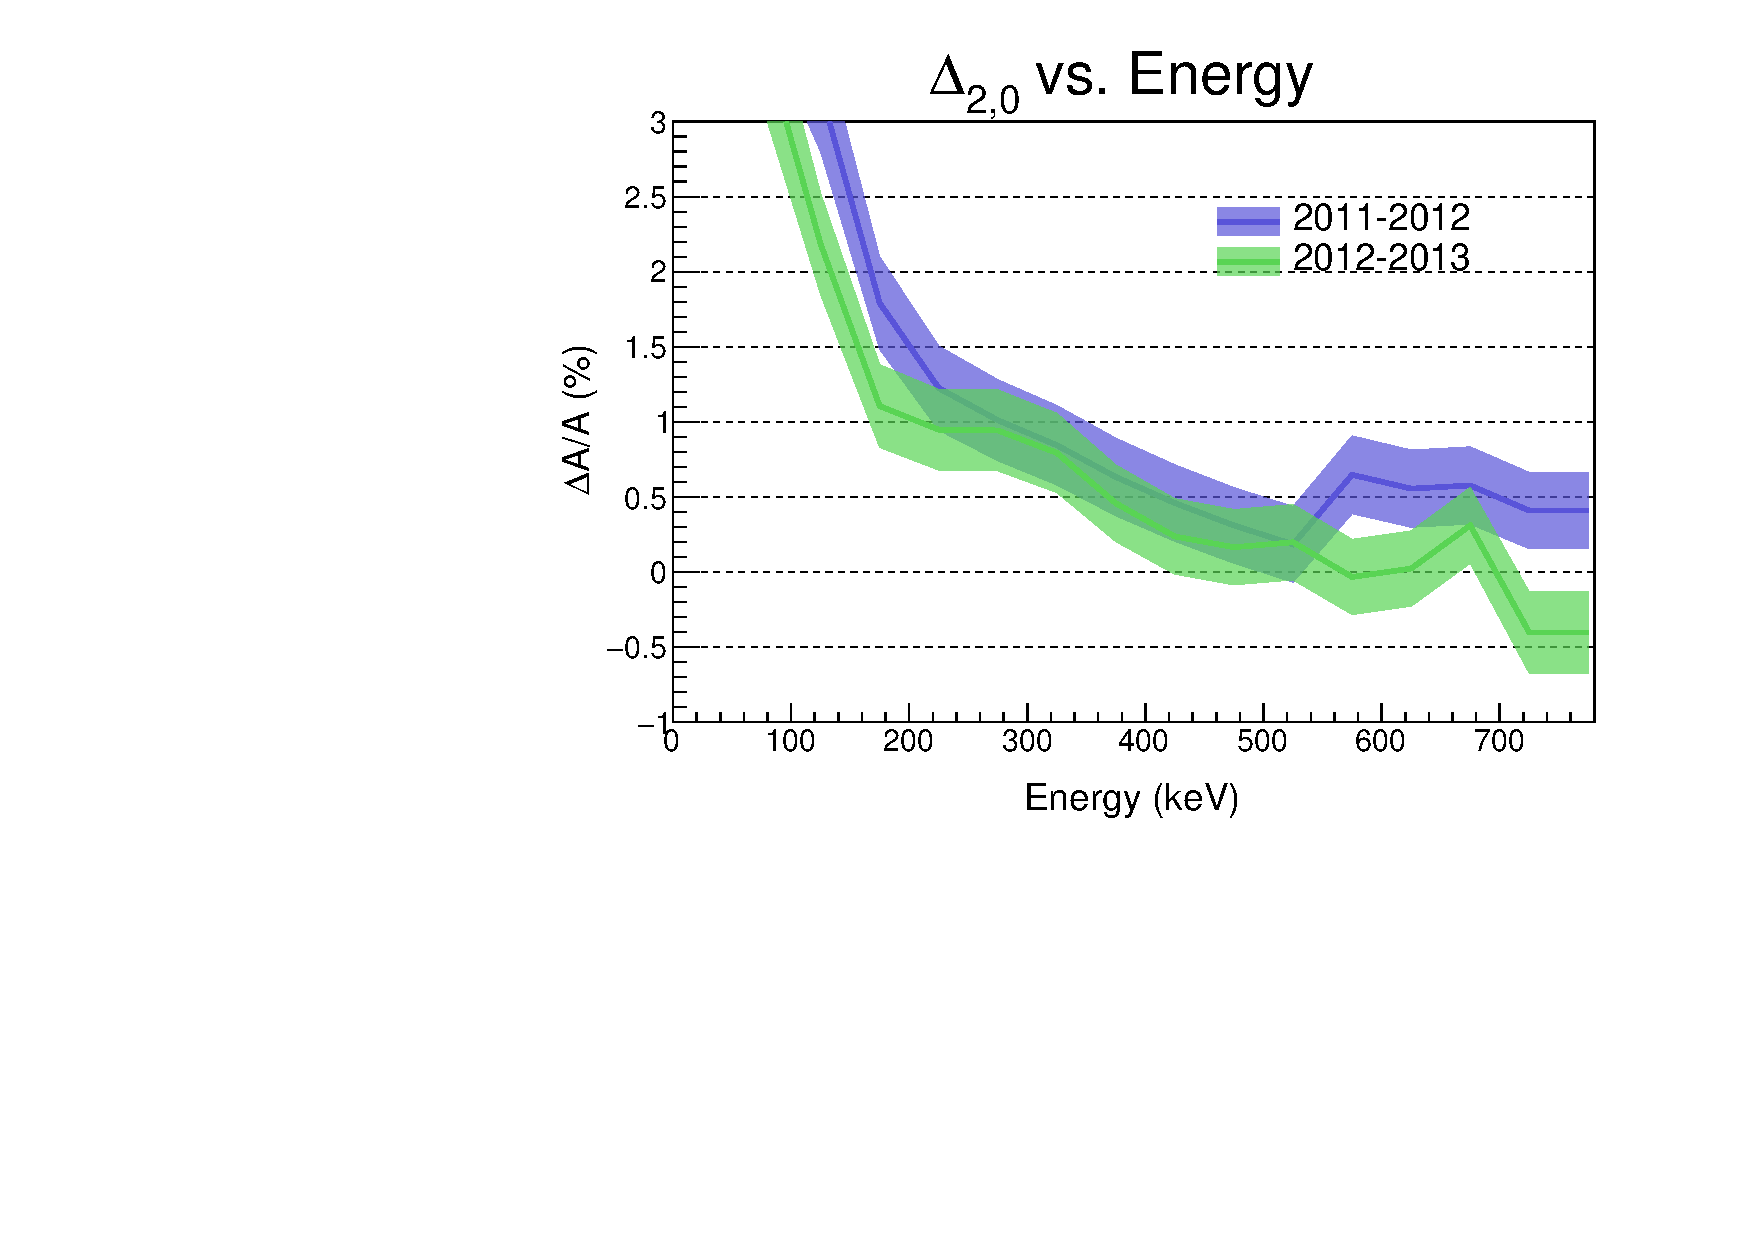
\includegraphics[page=1,scale=0.35]{5-UCNAResults/Delta_2_byType_anaChC_5BinAve_color.pdf}}&
    \subfloat[caption]{\includegraphics[page=2,scale=0.35]{5-UCNAResults/Delta_2_byType_anaChC_5BinAve_color.pdf}}
  \end{tabular}
  \begin{tabular} {cc}
    \subfloat[caption]{\includegraphics[page=3,scale=0.35]{5-UCNAResults/Delta_2_byType_anaChC_5BinAve_color.pdf}}&
    \subfloat[caption]{\includegraphics[page=4,scale=0.35]{5-UCNAResults/Delta_2_byType_anaChC_5BinAve_color.pdf}}
  \end{tabular}
  \subfloat[caption]{\includegraphics[page=5,scale=0.35]{5-UCNAResults/Delta_2_byType_anaChC_5BinAve_color.pdf}}
  \caption{Backscattering corrections for analysis choice used in final asymmetry extraction
    (All event types included with 2/3 separated using
    the MWPC energy calibration).}
  \label{fig:delta2}
\end{figure}

The corrections as a function of electron energy can be seen in figure
\ref{fig:delta2}.  Application of the correction increases
the magnitude of the measured asymmetry as it should, as missed backscattering events
dilute the measured asymmetry. The uncertainties seen in the figure
will be discussed in Section \ref{sssec:mcuncert}.
The leading contribution to the backscattering correction
comes from Type 0 events due to them accounting for roughly
$95\%$ of the data. The other event types have much smaller contributions to
the backscattering correction when all event types are included in the analysis
due primarily to the little statistical weight they carry. If the Type 0 events
are ignored, the backscattering corrections become very large for the Type 1, 2,
and 3 events. This will be illustrated when showing asymmetries for different
combinations of event types later in this chapter.


\begin{figure}[h]
  \centering
  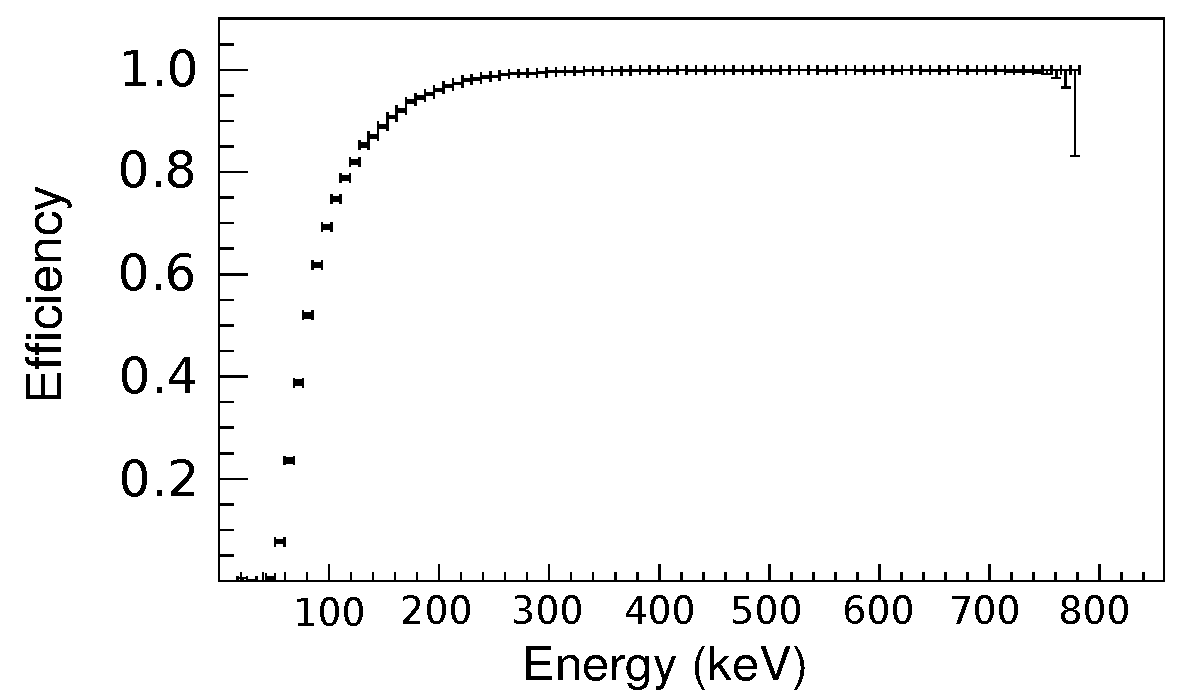
\includegraphics[scale=0.40]{5-UCNAResults/efficiency.pdf}  
  \caption{Simulated detector efficiency as a function of electron energy for electrons which
  pass through the decay trap endcaps.}
  \label{fig:effic}
\end{figure}

The difference between 2011-2012 and 2012-2013 corrections arises from the thinner
decay trap windows in 2012-2013, which substantially reduces the $\Delta_{2,0}$
correction for
misidentified Type 0 events. There is almost no effect on the other event types, as should
be expected due to no dramatic change in event type fractions or triggering efficiencies
for the two detector sides. Another way to think of this is that once an event passes through the
decay trap endcap, it's likelihood of triggering the detector approaches $100\%$ fairly quickly
(see Figure \ref{fig:effic}) and is not dependent on the changing geometry, so the corrections for
backscattering events are robust. Differing endcap thicknesses do however modify the number of misidentified
Type 0 events, decreasing them in the case of thinner windows as more electrons should pass through without
scattering, thus decreasing the magnitude of the
$\Delta_{2,0}$ correction by definition.


\subsubsection{Angular Acceptance, $\Delta_{3}$} \label{sssec:cosThetaCorr}
Remember from Equation \ref{eq:simpleRate} that the asymmetric
component of the decay rate depends on
$\beta\cos\theta$ and that we proceeded to integrate over one hemisphere
of the detector giving $\langle\cos\theta\rangle=1/2$. We also use the midpoint
of the energy bin of interest when evaluating $\beta=v/c$, which isn't equal to the
average value in a single bin due to the non-constant shape of the electron energy
spectrum. What is described is
an approximation of the form $\langle\beta\cos\theta\rangle \approx \beta_{\mathrm{mid}}/2$. The actual
value of $\langle\beta\cos\theta\rangle$ must be determined using simulated
data, as events are lost in an energy and angle dependent manner, with lower energy and
high pitch angle events being most likely to be lost. $\Delta_{3}$ attempts to
remove this angular dependence on event acceptance while also correcting for the slight
systematic effect of approximating $\beta$ at the midpoint.

If we define the asymmetry which properly accounts for the true $\langle\beta\cos\theta\rangle$
as $A'$ and the asymmetry which uses our approximation
$\langle\beta\cos\theta\rangle \approx \beta_{\mathrm{mid}}/2$ as $A$, then we see from
\ref{eq:A_SR} that
%
\begin{equation} \label{eq:ap}
  A' = \frac{A_{\mathrm{SR}}}{\langle\beta\cos\theta\rangle \langle P \rangle}
\end{equation}
%
\noindent and
%
\begin{equation} \label{eq:a}
  A = \frac{A_{\mathrm{SR}}}{\frac{\beta}{2} \langle P \rangle}.
\end{equation}
%
\noindent Then from our generic definition for a systematic correction, equation
\ref{eq:delta}, we have
%
\begin{equation*}
\Delta_3(E) = \frac{A'}{A}-1
\end{equation*}
%
\noindent and upon use of equations \ref{eq:ap} and \ref{eq:a},
%
\begin{equation} \label{eq:delta3def}
\Delta_3(E) = \frac{\frac{\beta}{2}}{\langle\beta\cos\theta\rangle}-1\textrm{ .}
\end{equation}
%
\noindent From this, we see that it is sufficient to determine $\langle\beta\cos\theta\rangle$
from simulation and calculate the energy dependent corrections.

\begin{figure}[h]
  \centering
  \begin{tabular} {cc}
    \subfloat[caption]{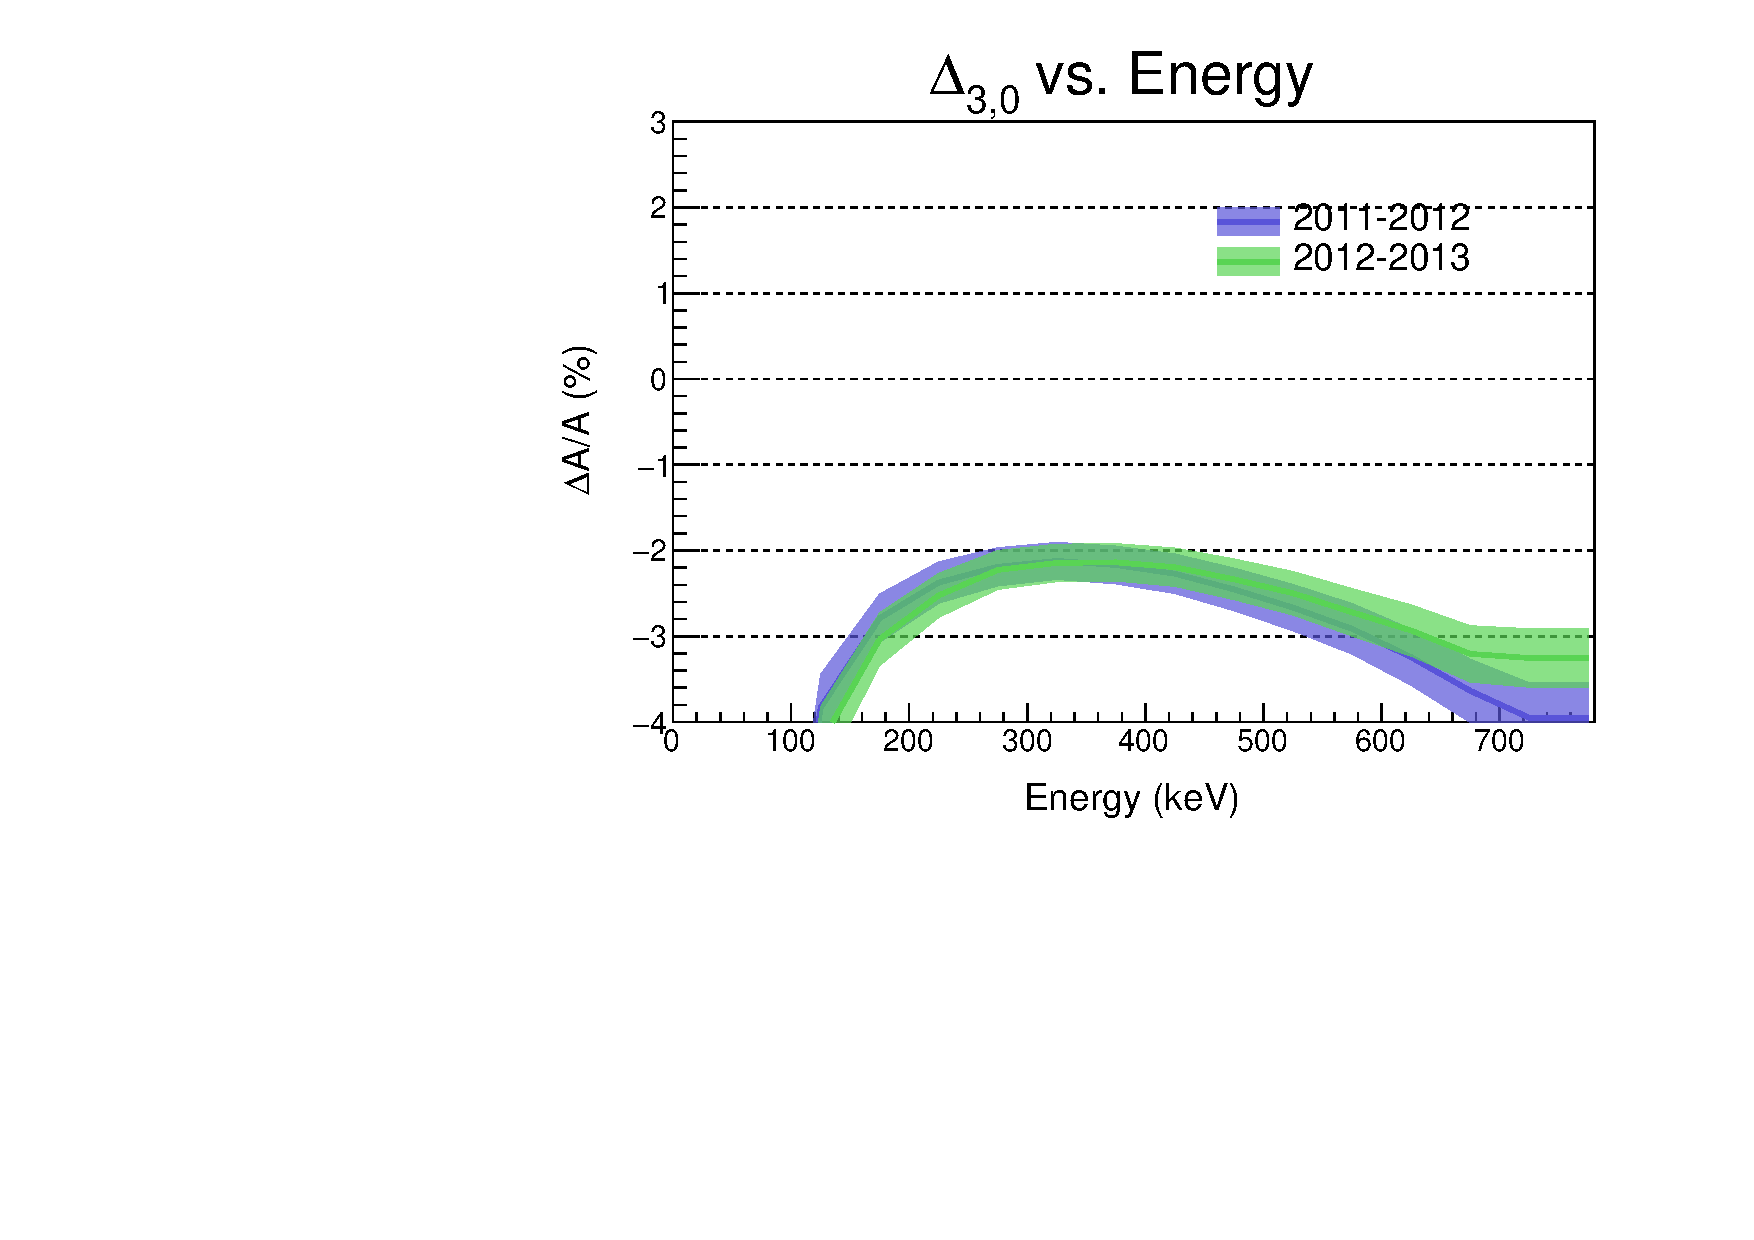
\includegraphics[page=1,scale=0.35]{5-UCNAResults/Delta_3_byType_anaChC_5BinAve_color.pdf}}&
    \subfloat[caption]{\includegraphics[page=2,scale=0.35]{5-UCNAResults/Delta_3_byType_anaChC_5BinAve_color.pdf}}
  \end{tabular}
  \begin{tabular} {cc}
    \subfloat[caption]{\includegraphics[page=3,scale=0.35]{5-UCNAResults/Delta_3_byType_anaChC_5BinAve_color.pdf}}&
    \subfloat[caption]{\includegraphics[page=4,scale=0.35]{5-UCNAResults/Delta_3_byType_anaChC_5BinAve_color.pdf}}
  \end{tabular}
  \subfloat[caption]{\includegraphics[page=5,scale=0.35]{5-UCNAResults/Delta_3_byType_anaChC_5BinAve_color.pdf}}
  \caption{$\cos\theta$ corrections for analysis choice used in final asymmetry extraction
    (All event types included with 2/3 separated using
    the MWPC energy calibration).}
  \label{fig:delta3}
\end{figure}
%
%\begin{figure}[h]
%  \centering
%  \includegraphics[page=7,scale=0.35]{5-UCNAResults/Delta_2_byType_anaChC_5BinAve_color.pdf}
%  \caption{Here is a caption}
%  \label{fig:deltaMC}
%\end{figure}
%

In previous analyses, this correction was done for the event population as a whole, producing
only a single correction $\Delta_3$. New work specific to this thesis allows for
separation of this correction into individual contributions from each event type,
%
\begin{equation}
1+\Delta_{3} = (1+\Delta_{3,3})(1+\Delta_{3,2})(1+\Delta_{3,1})(1+\Delta_{3,0}).
\end{equation}
%
\noindent This is more difficult than separating $\Delta_2$, as it requires more than a simple
event-by-event reassignment to the proper initial direction. This requires evaluation of
an average observable in the simulation, so we need a way to realize the contribution
of each event type to the average. The key is to use the individual asymmetry of each event
type and its respective angular correction, and then define the total correction as a function
of the individual corrections. 

Determination of the $\Delta_{3,i}$ corrections starts with a new definition of the
uncorrected combined asymmetry\footnote{\label{fnote:newAsymmDef}This definition
of the asymmetry is only used for analysis of this correction, and not for extraction
of the final asymmetry.} involving the individual asymmetries of each event type.
The following definitions will be useful in this derivation.
%
\begin{align*}
  &A \equiv \textrm{Uncorrected total asymmetry}\\
  &A^i \equiv \textrm{Asymmetry for event type } i\\
  &f^i \equiv \textrm{Statistical weight for event type }i\\
  &\Delta^i_3 \equiv \textrm{Angle correction to }A^i\textrm{ for event type }i\\
  &A^{\mathrm{corr},i} \equiv \textrm{Corrected asymmetry for event type } i\\
  &A_{\mathrm{corr},i} \equiv \textrm{Total asymmetry corrected for event type } i\\
  &\Delta_{3,i} \equiv \textrm{Angle correction to total asymmetry }A
  \textrm{ for event type }i
\end{align*}
%

Now we can define the uncorrected total asymmetry as
%
\begin{equation}
A=\sum_i f^iA^i
\end{equation}
%
\noindent where the sum runs over the event types that are to be included in the
determination of the asymmetry. As will be seen in \ref{sssec::anaChoices}, one can include
any combination of event types to produce many different asymmetries, so this definition
allows for use across any choice of event types.

Next we can define $\Delta^i_3$, or the angle correction to the asymmetry when only
including type $i$ events, using Equation \ref{eq:delta3def} and only including
type $i$ events when calculating $\langle\beta\cos\theta\rangle$. Then we can write down
an expression for the corrected asymmetry for that event type as
%
\begin{equation}
A^{\mathrm{corr},i} = (1+\Delta^i_3)A^i.
\end{equation}

It then follows that the total asymmetry corrected for the same event type $i$ becomes
%
\begin{equation}
A_{\mathrm{corr},i} = A^{\mathrm{corr},i} + \sum_{j\neq i} f^jA^j.
\end{equation}

With these relationships at hand, it is straightforward to follow the prescription to write
down an expression for $\Delta_{3,i}$ in terms of known values:
%
\begin{equation*}
  \Delta_{3,i} = \frac{A_{\mathrm{corr},i}}{A} - 1 = \frac{A_{\mathrm{corr},i}-A}{A} =
  \frac{f^i(A^{\mathrm{corr},i}-A^i)}{A}
\end{equation*}
%
\begin{equation}
  \Rightarrow\Delta_{3,i} = \frac{f^iA^i}{A}\Delta^i_3.
\end{equation}
%

The energy dependent $\Delta_{3,i}$ corrections are shown in Figure \ref{fig:delta3}.
The impact of applying the combined $\Delta_{3}$ correction is to decrease the magnitude of the
measured asymmetry. This comes from the dominance of the $\Delta_{3,0}$ portion, or the correction
due to the acceptance of Type 0 events. Type 0 events are more likely lost when they are high pitch
angle, low energy events. Such events carry little asymmetry information ($\beta\cos\theta$ gets small)
as seen in Equation \ref{eq:simpleRate}. Measurement of an asymmetry which has these low-asymmetry events
removed yields a larger magnitude asymmetry, thus necessitating a correction which decreases the
magnitude of the measured asymmetry. The contribution of the backscattering events to the angular
correction have the opposite sign and act to increase the magnitude of the measured asymmetry.
While this may seem counterintuitive due to the detectors nominally preferentially selecting
low pitch angle, high energy events, this sign is due to the backscattering events being overwhelmingly
high pitch angle events. Therefore $|\langle\cos\theta\rangle|$ over one hemisphere of the decay trap
will be less than the nominal value $1/2$ for all
backscattering events types, calling for a correction which increases the magnitude of the measured
asymmetry.

\subsubsection{Uncertainty in $\Delta_{\mathrm{MC}}$} \label{sssec:mcuncert}

In the analysis of the previous 2010 data set \cite{mendenhall2013} a
conservative 25\% uncertainty was applied to all Monte Carlo corrections, where the
25\% came from the observed discrepancy between data and Monte Carlo backscattering
fractions.  
The issue with such a correction is obvious when the correction itself is zero, as
any percent uncertainty on that correction would also be zero. One might argue that
the absence of a correction would imply the absence of an uncertainty in that correction,
but we must remember that the corrections are determined using Monte Carlo simulations
of finite statistics, thus even a 0\% correction comes with an uncertainty.
Another concern is that not all event type fractions disagree with Monte Carlo by
25\%, and the backscattering spectra that do disagree contribute little statistically
to the asymmetry. Also, the asymmetry is no longer dominated by statistical uncertainty,
and, as will be seen in Section \ref{ssec:energyRecon}, the uncertainty due to energy
reconstruction has been reduced, thus the ultra conservative worst-case scenario may
artificially limit our result.
With these  concerns taken into consideration, a new method was developed to assess
the uncertainty on the Monte Carlo corrections motivated by the fractional discrepancies
between data and simulation for each event type, denoted by $\delta_{\mathrm{frac}}\Delta_{i,j}$,
and the statistical fluctuations in the
corrections themselves, $\delta_{\mathrm{stat}}\Delta_{i,j}$.
%
\begin{figure}[h]
  \centering
  \begin{tabular} {cc}
    \subfloat[$\Delta_{2,0}$]{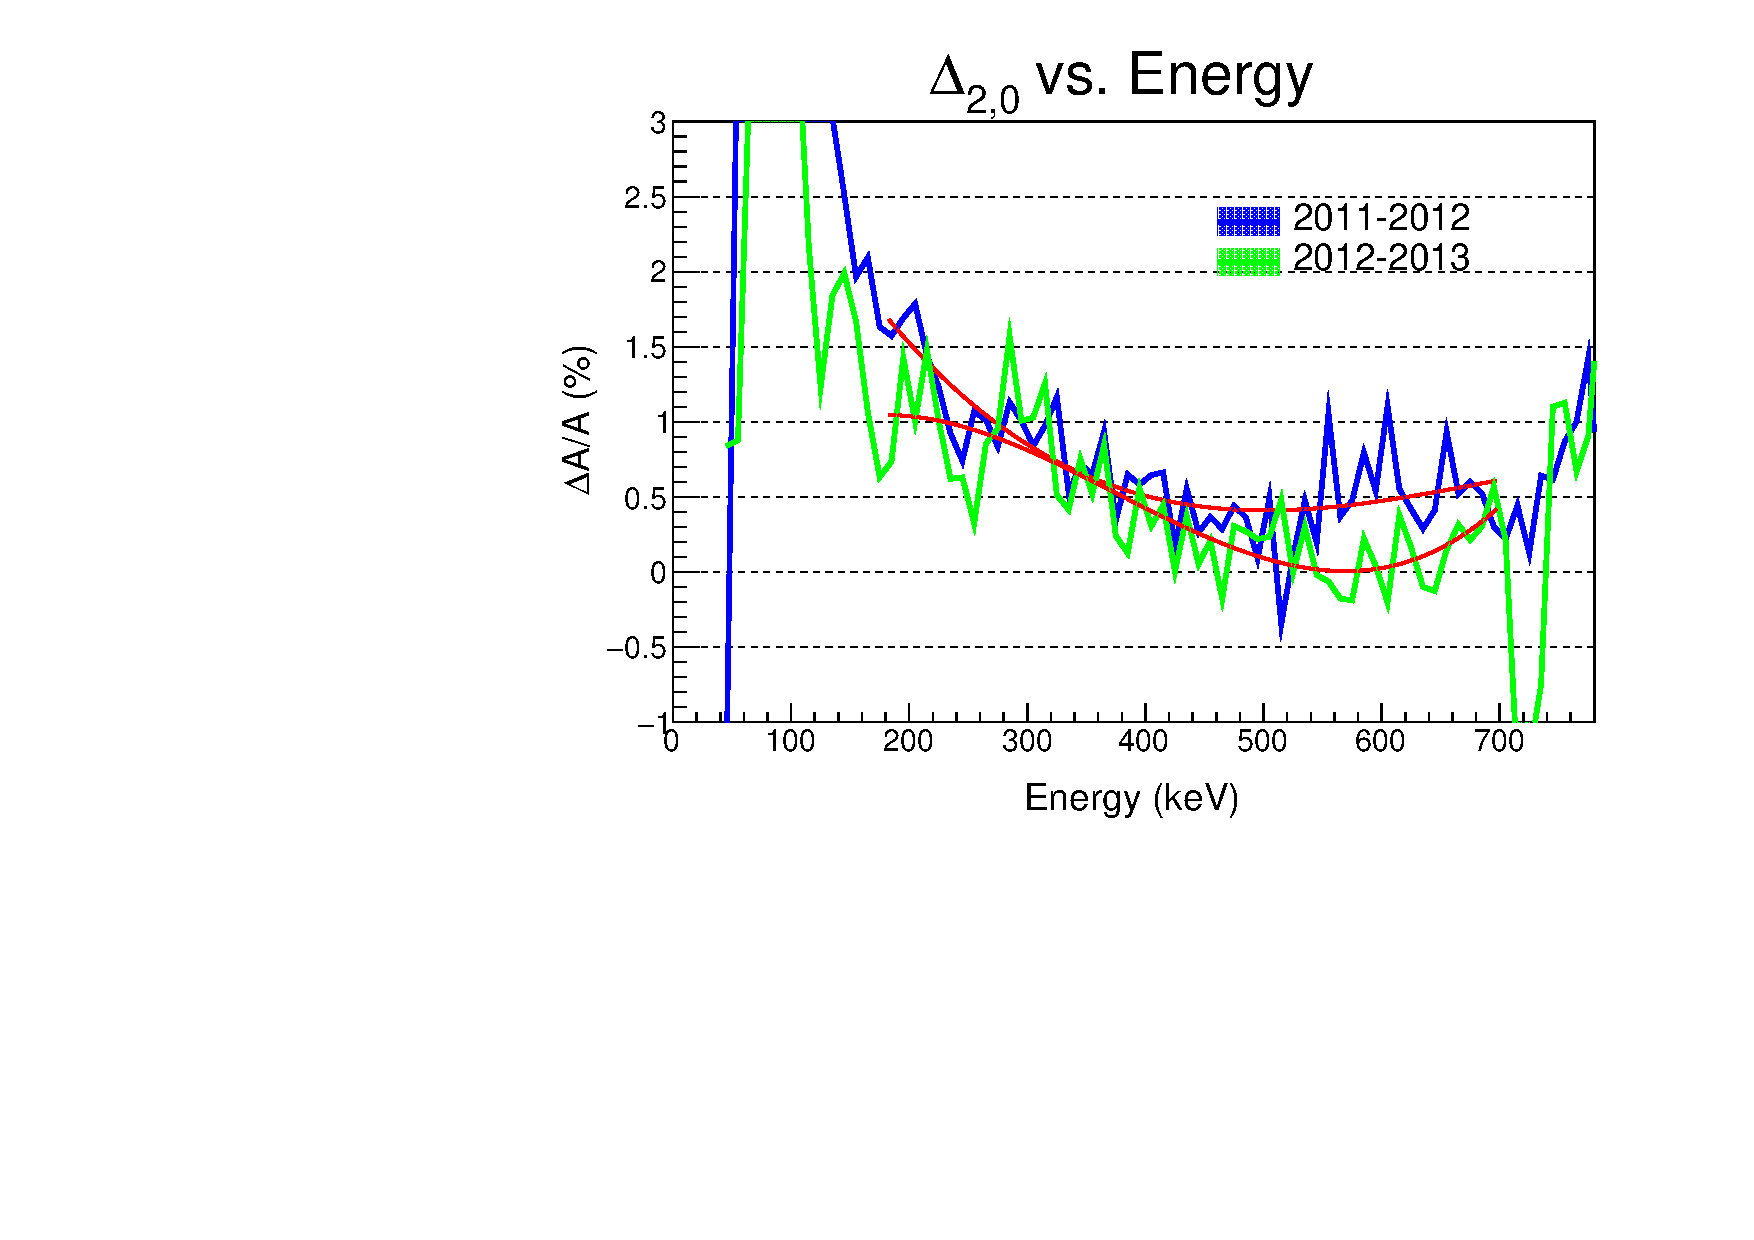
\includegraphics[page=1,scale=0.32]{5-UCNAResults/MC_Fits_anaChC.pdf}}&
    \subfloat[$\Delta_{2,1}$]{\includegraphics[page=2,scale=0.32]{5-UCNAResults/MC_Fits_anaChC.pdf}}
  \end{tabular}
  \begin{tabular} {cc}
    \subfloat[$\Delta_{2,2}$]{\includegraphics[page=3,scale=0.32]{5-UCNAResults/MC_Fits_anaChC.pdf}}&
    \subfloat[$\Delta_{2,3}$]{\includegraphics[page=4,scale=0.32]{5-UCNAResults/MC_Fits_anaChC.pdf}}
  \end{tabular}
  \caption{Bin-by-bin $\Delta_2$ corrections  with
    polynomial fit shown in red.}
  \label{fig:effStat}
\end{figure}
%
\begin{figure}[h]
  \centering
  \begin{tabular} {cc}
    \subfloat[$\Delta_{3,0}$]{\includegraphics[page=5,scale=0.32]{5-UCNAResults/MC_Fits_anaChC.pdf}}&
    \subfloat[$\Delta_{3,1}$]{\includegraphics[page=6,scale=0.32]{5-UCNAResults/MC_Fits_anaChC.pdf}}
  \end{tabular}
  \begin{tabular} {cc}
    \subfloat[$\Delta_{3,2}$]{\includegraphics[page=7,scale=0.32]{5-UCNAResults/MC_Fits_anaChC.pdf}}&
    \subfloat[$\Delta_{3,3}$]{\includegraphics[page=8,scale=0.32]{5-UCNAResults/MC_Fits_anaChC.pdf}}
  \end{tabular}
  \caption{Bin-by-bin $\Delta_3$ corrections with
    polynomial fit shown in red.}
  \label{fig:effStatDelta3}
\end{figure}

We further break up the statistical uncertainty
into two parts and add these in quadrature to get $\delta_{\mathrm{stat}}\Delta_{i,j}$.
There is an obvious uncertainty
that comes from simply propagating the statistics of the simulation through the correction,
which we will call
$\delta^{\mathrm{pure}}_{\mathrm{stat}}\Delta_{i,j}$.
This uncertainty doesn't seem to account for the fluctuations we see in the correction though, as
seen in Figure \ref{fig:effStat} panel (a) where the correction, when plotted for each
energy bin, oscillates at the roughly 0.25\% correction level at higher energies. This
oscillation may be due to correlations between the Monte Carlo events used to simulate each
run, as there are only 200 million events for each geometry and the events are chosen
randomly from this pool of events. Regardless of the cause, we account
for this observed statistical fluctuation using what we call the effective statistical
uncertainty, or $\delta^{\mathrm{eff}}_{\mathrm{stat}}\Delta_{i,j}$, which gives us
%
\begin{equation*}
  \delta \Delta_{i,j} = \sqrt{ (\delta_{\mathrm{frac}}\Delta_{i,j})^2 + ( \delta_{\mathrm{stat}}\Delta_{i,j})^2}
\end{equation*}
%
\begin{equation}
  \delta \Delta_{i,j} = \sqrt{ (\delta_{\mathrm{frac}}\Delta_{i,j})^2 +
    ( \delta^{\mathrm{pure}}_{\mathrm{stat}}\Delta_{i,j})^2 +
    ( \delta^{\mathrm{eff}}_{\mathrm{stat}}\Delta_{i,j})^2} .
\end{equation}

\setlength{\tabcolsep}{12pt}

\begin{table}[h]
  \caption{Values for the effective statistical uncertainties from each
  event type. The value is reported as the uncertainty on $\frac{\Delta A}{A}$.} 
  \centering
  \begin{tabular}{l c }
    \hline \hline \\ [-1.75ex]
    & \% Uncert. \\
    \hline \\ [-1.75ex]
    $\delta^{\mathrm{eff}}_{\mathrm{stat}}\Delta_{2,0}$ & $\pm0.25$ \\ [0.50ex]
    $\delta^{\mathrm{eff}}_{\mathrm{stat}}\Delta_{2,1}$ & $\pm0.074$ \\ [0.50ex]
    $\delta^{\mathrm{eff}}_{\mathrm{stat}}\Delta_{2,2}$ & $\pm0.062$ \\ [0.50ex]
    $\delta^{\mathrm{eff}}_{\mathrm{stat}}\Delta_{2,3}$ & $\pm0.059$  \\ [0.50ex]
    \hline \\ [-1.75ex]
    $\delta^{\mathrm{eff}}_{\mathrm{stat}}\Delta_{3,0}$ & $\pm0.04$ \\ [0.50ex]
    $\delta^{\mathrm{eff}}_{\mathrm{stat}}\Delta_{3,1}$ & $\pm0.04$ \\ [0.50ex]
    $\delta^{\mathrm{eff}}_{\mathrm{stat}}\Delta_{3,2}$ & $\pm0.02$ \\ [0.50ex]
    $\delta^{\mathrm{eff}}_{\mathrm{stat}}\Delta_{3,3}$ & $\pm0.02$  \\ [0.50ex]
    \hline
  \end{tabular}
  \label{tab:effStat}
\end{table}

To determine the effective statistical uncertainty $\delta^{\mathrm{eff}}_{\mathrm{stat}}\Delta_{i,j}$,
we begin by fitting the bin-by-bin Monte Carlo corrections with the combination of a decaying exponential
and a third-order polynomial,
%
\begin{equation}
  f(E) = C_0 e^{-C_1E} + C_2 + C_3E + C_4E^2 + C_5E^3.
\end{equation}
%
The decaying exponential is included to describe the expected larger correction at low
energies for backscattering which tapers off as energy increases (remember that the lower
energy events are more likely to backscatter). The polynomial is included to account for
any other observed shape in the corrections. The function was initially developed for use
on the $\Delta_{\mathrm{2}}$ corrections, but the same functional fit worked well for
$\Delta_{\mathrm{3}}$ and thus was adopted for both corrections.

After fitting the corrections, one can form residuals for every energy bin by subtracting the actual value
of the correction from the value given by the fit. The RMS of the residuals was
then calculated
separately for each $\Delta_{i,j}$ and each geometry. The effective statistical uncertainty
was set to the larger RMS from the two geometries for each $\Delta_{i,j}$ to be conservative.
The values for $\delta^{\mathrm{eff}}_{\mathrm{stat}}\Delta_{i,j}$
can be found in table \ref{tab:effStat}.

\setlength{\tabcolsep}{12pt}

\begin{table}[h]
  \caption{Values for the fractional uncertainties from each
  event type. The value is reported as the uncertainty on $\frac{\Delta A}{A}$.} 
  \centering
  \begin{tabular}{l c }
    \hline \hline \\ [-1.75ex]
    & \% Uncert. \\
    \hline \\ [-1.75ex]
    $\delta_{\mathrm{frac}}\Delta_{2,0}$ & $\pm0.10$ \\ [0.50ex]
    $\delta_{\mathrm{frac}}\Delta_{2,1}$ & $\pm0.30$ \\ [0.50ex]
    $\delta_{\mathrm{frac}}\Delta_{2,2}$ & $\pm0.40$ \\ [0.50ex]
    $\delta_{\mathrm{frac}}\Delta_{2,3}$ & $\pm0.20$  \\ [0.50ex]
    \hline \\ [-1.75ex]
    $\delta_{\mathrm{frac}}\Delta_{3,0}$ & $\pm0.10$ \\ [0.50ex]
    $\delta_{\mathrm{frac}}\Delta_{3,1}$ & $\pm0.30$ \\ [0.50ex]
    $\delta_{\mathrm{frac}}\Delta_{3,2}$ & $\pm0.40$ \\ [0.50ex]
    $\delta_{\mathrm{frac}}\Delta_{3,3}$ & $\pm0.20$  \\ [0.50ex]
    \hline
  \end{tabular}
  \label{tab:frac}
\end{table}

\begin{table}[h]
  \caption{Actual integrated event type fractions as percent of
    total events. Also reported is the \% difference between Monte Carlo and data
    spectra for each event type. These are calculated over an energy window of
    190-740~keV, chosen to minimize the total uncertainty as will be shown.} 
  \centering
  \begin{tabular}{l c c c c }
    \hline \hline \\ [-1.75ex]
     & Type 0 & Type 1 & Type 2 & Type 3 \\
    \hline \\ [-1.75ex]
    Data & $94.44$ & $3.31$ & $1.09$ & $1.15$  \\ [0.50ex]
    MC & $94.86$ & $3.30$ & $0.78$ & $1.06$  \\ [0.50ex]
    \% Diff. & $0.44$ & $-0.29$ & $-28.24$ & $-7.91$  \\ [0.50ex]    
    \hline
  \end{tabular}
  \label{tab:integratedFrac}
\end{table}

Assigning values for the fractional uncertainties on each correction is more straightforward
and comes from looking at the spectral discrepancies of each event type. We have a Monte
Carlo predicted spectrum and a data spectrum for each of our event types, so we can construct
a fractional residual between these spectra as seen in Figure \ref{fig:fracResid} simply using
$\frac{\mathrm{MC}}{\mathrm{Data}}-1$. Then by choosing approximately
the maximum fractional residual over energies of interest (180-700~keV, starting at roughly the lower
limit on our analysis energy window and ending when the statistics drop below 10\% of the maximum rate),
we conservatively set the fractional discrepancy of our corrections. The values of 
$\delta_{\mathrm{frac}}\Delta_{i,j}$ are tabulated in table \ref{tab:frac}.
One should note
that the integrated agreement between Monte Carlo and data is much better than these
conservative fractional uncertainties, as seen in table \ref{tab:integratedFrac}.

\begin{figure}[p]
  \centering
  \subfloat[Type 0]{\includegraphics[page=2,scale=0.48]{5-UCNAResults/spectraComp_0-121_TypeALL_190-740.pdf}} \\ [-0.3ex]
  \subfloat[Type 1]{\includegraphics[page=3,scale=0.48]{5-UCNAResults/spectraComp_0-121_TypeALL_190-740.pdf}} \\ [-0.3ex]
  \subfloat[Type 2]{\includegraphics[page=4,scale=0.48]{5-UCNAResults/spectraComp_0-121_TypeALL_190-740.pdf}} \\ [-0.3ex]
  \subfloat[Type 3]{\includegraphics[page=5,scale=0.48]{5-UCNAResults/spectraComp_0-121_TypeALL_190-740.pdf}}
  \caption{Subfigures are broken into each event type.
    Left of each subfigure shows electron energy spectra for background subtracted data (blue open circles),
    Monte Carlo (black solid line), and the background (black closed circles). The right plot in each
    subfigure shows the fractional residual between background subtracted data and Monte Carlo, which is used
    when applying the conservative fractional uncertainty on the Monte Carlo corrections.}
  \label{fig:fracResid}
\end{figure}

\subsubsection{Fidelity of Corrections}

As mentioned in Section \ref{sssec:betaSim}, an asymmetry equal to the
2017 PDG value ($A_0=-0.1184$) was incorporated into the Monte Carlo
event generator, along with all radiative and recoil order effects. This allows
us to extract the Monte Carlo corrections from event distributions which mimic
our measurement populations, but it also allows us to apply our corrections
to the Monte Carlo rates to see what we extract for $A_0$. Because we process
the simulations such that we have complementary simulated data for every
$\beta$-decay run (with the Monte Carlo having $\approx 16~\times$ data statistics),
we can run the simulated data through the same asymmetry extraction method and compare
the extracted fully-corrected asymmetry to the PDG input value. Figure \ref{fig:MCasymm}
shows the Monte Carlo corrected asymmetries for all analysis choices. The agreement across
all event types indicates the energy dependent Monte Carlo corrections are self-consistent.

\begin{figure}[h]
  \centering
  \begin{tabular} {c}
    \subfloat[2011-2012]{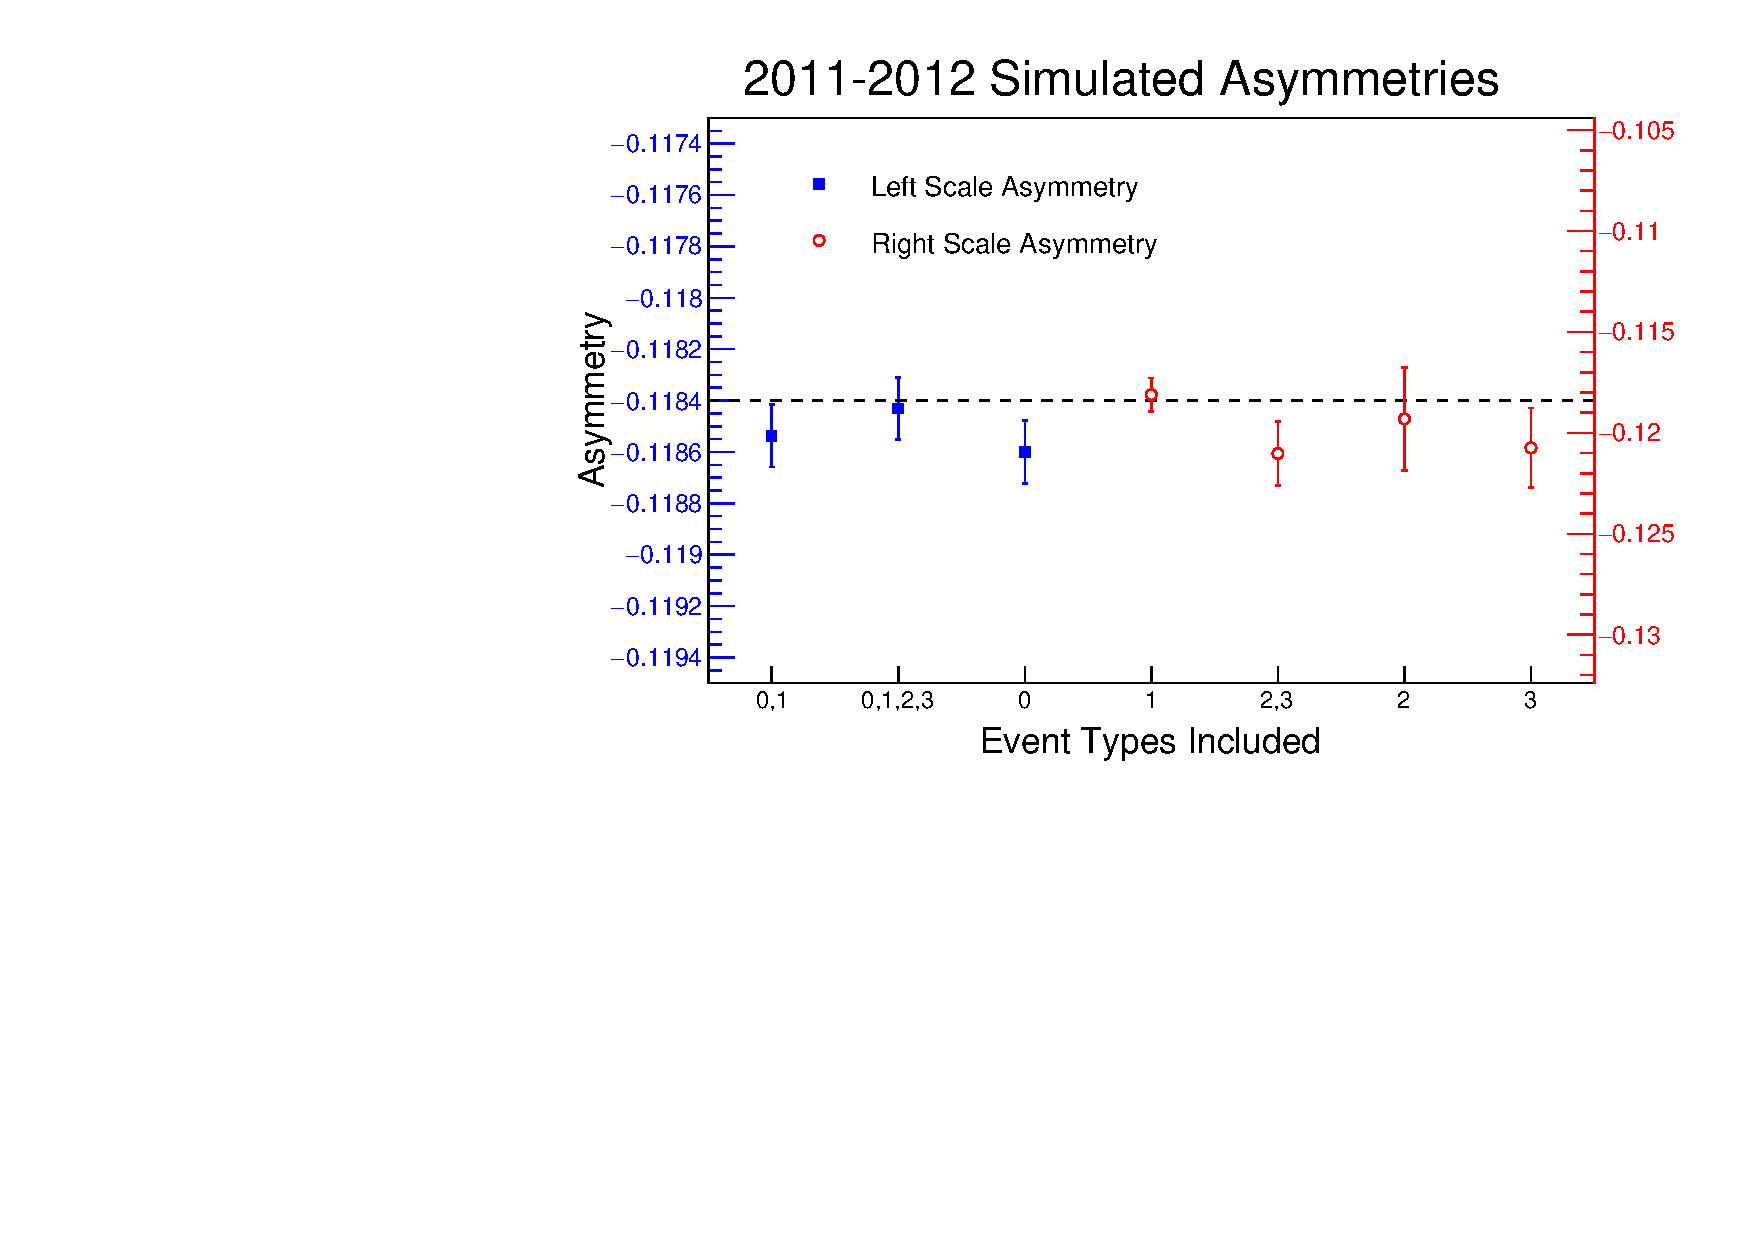
\includegraphics[page=1,scale=0.5]{5-UCNAResults/asymms_doubleAxis_AllCorr__color.pdf}} \\ 
    \subfloat[2012-2013]{\includegraphics[page=2,scale=0.5]{5-UCNAResults/asymms_doubleAxis_AllCorr__color.pdf}}
  \end{tabular}
  \caption{Extracted asymmetries from Monte Carlo data processed to mimic the
    experimental data. The dashed line indicates the 2017 PDG value $A_0 = -0.1184$
    which was input into the simulation, thus the goal upon extraction of the final
    asymmetry parameter. The blue closed points indicate analysis choices that include
    type 0 events and utilize the scale on the left vertical axis values. The red open circles
    include only backscattering event types and use the right vertical axis values.}
  \label{fig:MCasymm}
\end{figure}


\subsection{Polarimetry Correction} \label{ssec:polCorr}

As mentioned in Section \ref{sec:polarimetry}, an equilibrium population of neutron
spins develops within the decay trap during a $\beta$-decay run. While this population is
dominated by the spin-state of choice ($>99\%$), precise determination of the average
polarization is important as it directly affects the final extracted asymmetry as shown in
equation \ref{eq:A0}. The determination of the polarization values was carried
out in a separate analysis by Eric Dees of North Carolina State University.
The values for the $\pm$ spin-flipper states for
each geometry are given in table \ref{tab:pol}.

\setlength{\tabcolsep}{12pt}
\begin{table}[h]
  \caption{Results for average polarization fractions for each dataset in spin-flipper off ($-$)
    and spin-flipper on ($+$) states.} 
  \centering
  \begin{tabular}{c c c c}
    \hline \hline \\ [-1.75ex]
    \multicolumn{2}{c}{2011-2012}&\multicolumn{2}{c}{2012-2013} \\ [0.5ex]
    $\langle P \rangle_-$ & $\langle P \rangle_+$ & $\langle P \rangle_-$ & $\langle P\rangle_+$ \\ [0.25ex]
    \hline \\ [-1.75ex]
    %$\Delta P/P$ (\%) & 0.30 & 0.25 & 0.15 & 0.20 \\ [0.25ex]
    0.9970(30) & 0.9939(25) & 0.9979(15) & 0.9952(20) \\ [0.25ex]
    \hline
  \end{tabular}
  \label{tab:pol}
\end{table}

There are two options for applying a polarization correction, namely
calculate an average polarization $\langle P \rangle$
which is averaged over both spin states and simply
divide this out of the measured asymmetry as shown in Equation \ref{eq:A0}, or utilize the
separate $\langle P\rangle_\pm$ values. The second method is not a simple division of
either term but rather a more complicated combination due to the usage of the super-ratio.
This second method was adopted for this analysis and is described below.

\subsubsection{Extraction of $A_0$ Using $\langle P \rangle_+$ and $\langle P \rangle_-$}
\label{ssec:polSep}

Using each of the $\langle P\rangle_\pm$ values requires modification of our initial
asymmetry formalism from \ref{sec:asymmetry} \cite{ARYoungPol}. We can no longer make
the assumption that $\langle P\rangle_+ = \langle P\rangle_-$ if we want to treat them
separately. Let us start our new derivation from Equation \ref{eq:decayRate}, which now
becomes
%
\begin{equation} \label{eq:POLdecayRate}
  \Gamma_{1,2}^{\pm}\left(E\right)=C' \cdot S(E) \cdot \epsilon_{\pm} \cdot \eta_{1,2}
  \left[ 1 \pm_{1,2} 
    \left(\mp \langle P \rangle_\pm \right) \cdot A(E) \frac{\beta}{2} \right]
\end{equation}
%
\noindent under the substition $\langle P\rangle \rightarrow \langle P\rangle_\pm$.

The super-ratio now must be written as
%
\begin{equation*}
  R = \frac{\Gamma_{1}^+ \cdot \Gamma_{2}^-}{\Gamma_{1}^- \cdot \Gamma_{2}^+} 
  =  \frac{ \left[ 1 + \left(- \langle P \rangle_+ \right)  A(E) \frac{\beta}{2} \right] 
\left[ 1 - \left(+ \langle P \rangle_- \right)  A(E) \frac{\beta}{2} \right]  }
{  \left[ 1 +  \left(+ \langle P \rangle_- \right)  A(E) \frac{\beta}{2}  \right] 
 \left[ 1 -  \left(- \langle P \rangle_+ \right)  A(E) \frac{\beta}{2} \right]},
\end{equation*}
%
\noindent and upon letting $\xi = A(E)\frac{\beta}{2}$ we have
%
\begin{equation} \label{eq:polR}
  R =  \frac{ \Big( 1 - \xi \langle P \rangle_+ \Big)
    \Big( 1 - \xi \langle P \rangle_- \Big) }
{  \Big( 1 + \xi \langle P \rangle_- \Big)
    \Big( 1 + \xi \langle P \rangle_+ \Big) }.
\end{equation}

We are interested in solving for $A(E)$, or $\xi$, so we can rearrange \ref{eq:polR} to give
%
\begin{equation*}
  R\Big( 1 + \xi \langle P \rangle_- \Big) \Big( 1 + \xi \langle P \rangle_+ \Big) =
  \Big( 1 - \xi \langle P \rangle_+ \Big)
    \Big( 1 - \xi \langle P \rangle_- \Big),
\end{equation*}
%
\begin{equation*}
  R\bigg( 1 + \xi \Big(\langle P \rangle_-+\langle P \rangle_+ \Big) + \xi^2\langle P \rangle_-
  \langle P \rangle_+\bigg) =
  \bigg( 1 - \xi \Big(\langle P \rangle_-+\langle P \rangle_+ \Big) + \xi^2\langle P \rangle_-
  \langle P \rangle_+\bigg),
\end{equation*}
%
\begin{equation*}
  0 = \xi^2\langle P \rangle_- \langle P \rangle_+\Big(1-R\Big)
  - \xi\Big(\langle P \rangle_-+\langle P \rangle_+ \Big)\Big(1+R\Big)
  + \Big(1-R\Big),
\end{equation*}
%
\noindent and
%
\begin{equation}
  0 = \xi^2\langle P \rangle_- \langle P \rangle_+
  - \xi\Big(\langle P \rangle_-+\langle P \rangle_+ \Big)\bigg(\frac{1+R}{1-R}\bigg)
  + 1,
\end{equation}
%
\noindent which has roots (let $\gamma = \frac{1+R}{1-R}$)
%
\begin{equation}
  \xi = \frac{\gamma\Big(\langle P \rangle_-+\langle P \rangle_+ \Big)
    \pm \sqrt{\gamma^2\Big(\langle P \rangle_-+\langle P \rangle_+ \Big)^2
      -4\langle P \rangle_- \langle P \rangle_+}}
      {2\langle P \rangle_- \langle P \rangle_+}.
\end{equation}

To choose the proper root, we set
$\langle P \rangle_- = \langle P \rangle_+ = \langle P \rangle$ and determine
which root returns the original expression for the super-ratio as given in equations
\ref{eq:A_SR_frac} and \ref{eq:A_SR}, namely
%
\begin{equation*} \label{eq:A_SR}
  A_{\mathrm{SR}} = \frac{1-\sqrt{R}}{1+\sqrt{R}} = \langle P
  \rangle  A(E)  \frac{\beta}{2}.
\end{equation*}
%
\noindent Upon doing so, we find that the negative root is the correct
solution, which results in a new expression for $A(E)$ of
%
\begin{equation}
  A(E) = \frac{\gamma\Big(\langle P \rangle_-+\langle P \rangle_+ \Big)
    - \sqrt{\gamma^2\Big(\langle P \rangle_-+\langle P \rangle_+ \Big)^2
      -4\langle P \rangle_- \langle P \rangle_+}}
      {\beta\langle P \rangle_- \langle P \rangle_+}.
\end{equation}

The uncertainty on $A(E)$ from such an application of the polarization is determined via
the usual error propagation,
%
\begin{equation}
  \delta_PA(E) = \sqrt{\bigg(\frac{\partial A(E)}{\partial \langle P \rangle_+}\bigg)^2
    \Big(\delta \langle P \rangle_+\Big)^2 +
    \bigg( \frac{\partial A(E)}{\partial \langle P \rangle_-}\bigg)^2
    \Big(\delta \langle P \rangle_-\Big)^2}.
\end{equation}
%
Although this method of determining the measured asymmetry is more rigorous than using a
polarimetry value averaged over the two spin states, the effect on the asymmetry is
at the $\Delta A \approx 10^{-6}$ level as shown by K. Hickerson in \cite{hickerson2013}.
A change in the asymmetry of this magnitude is small compared to the uncertainty from
the polarization alone and inconsequential compared
to the final uncertainty on the asymmetry. 


\subsection{Energy Reconstruction} \label{ssec:energyRecon}

The energy enters the calculation of the asymmetry in the $\beta$ term ($v/c$ of the
electron) in Equation \ref{eq:A_SR}, and thus it is essential to assess how well
we can reconstruct the initial energy of an electron. The obvious choice for determining
the efficacy of our energy calibration is to use the calibration peaks themselves and
compare to Monte Carlo simulation. We apply the calibrations from
Chapter \ref{ch:UCNA_Calibrations} to the data source peaks in all
individual source runs,
which maps the detector response to a reconstructed peak energy ($E_{\mathrm{recon}}^{\mathrm{data}}$),
and then we apply our
detector response model to the simulation peaks and extract a Monte Carlo reconstructed peak energy
($E_{\mathrm{recon}}^{\mathrm{MC}}$). We can then calculate a residual for every single run (and each
conversion peak within that run) via
$\mathrm{Residual} = E_{\mathrm{recon}}^{\mathrm{data}} - E_{\mathrm{recon}}^{\mathrm{MC}}$. Upon collecting all
of the residuals for each of the conversion electron peaks (Figures \ref{fig:residuals2011}
and \ref{fig:residuals2012}), we calculate
\footnote{ \label{fn:sourceMean}The mean and sigma are calculated rather than fitted so as to not neglect any
  non-Gaussian tails in the distributions.} the mean and sigma of the distributions, with
values reported in table \ref{tab:residuals}, and use
them as the data points seen in Figure \ref{fig:errEnv}. These points are a measure
of the accuracy of the energy calibration at four discrete energies, the mean energies of the
conversion electron lines themselves.

\begin{figure}[h]
  \centering
  \begin{tabular} {c c}
    \subfloat[$^{137}\mathrm{Ce}$ Conversion Line]{\includegraphics[page=11,scale=0.35]{5-UCNAResults/final_residuals_1-12.pdf}} &
    \subfloat[$^{113}\mathrm{Sn}$ Conversion Line]{\includegraphics[page=13,scale=0.35]{5-UCNAResults/final_residuals_1-12.pdf}} \\
    \subfloat[Lower $^{207}\mathrm{Bi}$ Conversion Line]{\includegraphics[page=14,scale=0.35]{5-UCNAResults/final_residuals_1-12.pdf}} &
    \subfloat[Upper $^{207}\mathrm{Bi}$ Conversion Line]{\includegraphics[page=15,scale=0.35]{5-UCNAResults/final_residuals_1-12.pdf}}
  \end{tabular}
  \caption{Distributions of the residuals for each conversion electron source line used in the 2011-2012 calibration.
    The mean and sigma reported in the fit box are not the same as those used in the energy uncertainty, as they
    are the results of the fit and not the calculated mean.}
  \label{fig:residuals2011}
\end{figure}

\begin{figure}[h]
  \centering
  \begin{tabular} {c c}
    \subfloat[$^{137}\mathrm{Ce}$ Conversion Line]{\includegraphics[page=11,scale=0.35]{5-UCNAResults/final_residuals_16-24.pdf}} &
    \subfloat[$^{113}\mathrm{Sn}$ Conversion Line]{\includegraphics[page=13,scale=0.35]{5-UCNAResults/final_residuals_16-24.pdf}} \\
    \subfloat[Lower $^{207}\mathrm{Bi}$ Conversion Line]{\includegraphics[page=14,scale=0.35]{5-UCNAResults/final_residuals_16-24.pdf}} &
    \subfloat[Upper $^{207}\mathrm{Bi}$ Conversion Line]{\includegraphics[page=15,scale=0.35]{5-UCNAResults/final_residuals_16-24.pdf}}
  \end{tabular}
  \caption{Distributions of the residuals for each conversion electron source line used in the 2012-2013 calibration.
    The mean and sigma reported in the fit box are not the same as those used in the energy uncertainty, as they
    are the results of the fit and not the calculated mean.}
  \label{fig:residuals2012}
\end{figure}

%\setlength{\tabcolsep}{12pt}
\begin{table}[h]
  \caption{Mean and $\sigma$ of each conversion electron residual distribution
  as used in the energy uncertainty, Figure \ref{fig:errEnv}.} 
  \centering
  \begin{tabular}{c c c}
    \hline \hline \\ [-1.75ex]
    & 2011-2012 & 2011-2012 \\
    \hline \\ [-1.75ex]
    $^{137}\mathrm{Ce}$ & $-1.43\pm1.81$~keV & $-0.80\pm2.00$~keV \\
    $^{113}\mathrm{Sn}$ & $0.91\pm2.52$~keV & $-2.24\pm2.87$~keV \\
    $^{207}\mathrm{Bi}$ (lower) & $-1.36\pm3.81$~keV & $-0.39\pm3.90$~keV \\
    $^{207}\mathrm{Bi}$ (upper) & $-1.55\pm5.77$~keV & $0.01\pm6.40$~keV \\
    \hline
  \end{tabular}
  \label{tab:residuals}
\end{table}

\begin{figure}[h]
\centering
\includegraphics[scale=.65]{5-UCNAResults/energyErrorEnvelope_color.pdf}
\caption{Plot of energy uncertainty vs. reconstructed energy. The points plotted are the mean
  and $\sigma$ of all reconstructed calibration peaks of $^{137}\mathrm{Ce}$,
  $^{113}\mathrm{Sn}$, and the lower and
  upper $^{207}\mathrm{Bi}$ peaks in that order. The $x$-axis offset in the 2011-2012 and 2012-2013 points is
  artificial and only meant for visualization. The bands represent the energy uncertainty
  at any given electron energy for the two data sets.}
\label{fig:errEnv}
\end{figure}

\begin{figure}[h]
\centering
\includegraphics[scale=.50]{5-UCNAResults/EnergyUncertALL.pdf}
\caption{Plot of uncertainty on $A_0$ from the energy calibration vs. reconstructed energy
  for each of the 2011-2012 and 2012-2013 geometries. Weighting the energy dependent
  uncertainties shown here by the experimental statistics in each energy bin produces
  the final uncertainty on the extracted asymmetries.}
\label{fig:energyUncert}
\end{figure}

The residuals at these discrete energies do not
themselves tell us how well we do at intermediate energies. In the past, a conservative
uncertainty envelope was drawn to encompass the calibration points
\cite{mendenhall2013,mpmThesis}. For the analysis
presented here, a more quantitative determination of the uncertainty envelope was employed
via methods developed by K. Hickerson for determination of limits on $b_n$ from the previous
UCNA spectrum (\cite{hickerson2017}). In short, the envelope is produced by sampling
the coefficients of a quadratic, $f(E_{\mathrm{recon}})$, from distributions that reproduce
the residual data points seen in Figure \ref{fig:errEnv} with $1\sigma$ deviation.
This
obviously results in an asymmetric uncertainty band due to the asymmetric distribution
of the data points about zero, but our conservative approach is
to take the worst case uncertainty at every energy and use this as our
symmetric final uncertainty.
This produces the symmetric uncertainty band in Figure \ref{fig:errEnv}.

The symmetric worst case uncertainty band allows us to report a systematic uncertainty
rather than a correction and an uncertainty from the energy reconstruction. The energy
dependent uncertainty on $A_0$ for the maximal energy uncertainty (outer edge of the
uncertainty envelope) is shown in Figure \ref{fig:energyUncert}.
The uncertainty is then weighted by the data statistics in each bin to determine the
total uncertainty in the final asymmetry, producing energy uncertainties of $0.17\%$ and
$0.25\%$ for 2011-2012 and 2012-2013 respectively.

\subsection{Background Contributions}

The desired events (foreground) are superposed with background
triggering events from something other
than a neutron $\beta$-decay within the decay trap. Such unwanted events include
background ambient
gamma rays, cosmic rays,
and other unforeseen events which trigger the detector.
Gamma ray events are highly suppressed due to the
requirement of a coincidence trigger between the MWPC and the scintillator,
and cosmic ray muon events are removed using a series of muon veto
detection packages, which leaves the rest of the background to be subtracted using direct
measurements of the electron spectrum in the absence of neutrons in the decay trap.

\subsubsection{Background Subtraction} \label{sssec:bgsubtr}

Accompanying every $\beta$-decay run is a dedicated background run roughly $1/4$ the
length of the data taking run. The background events are processed in an identical manner
to the data events and the rates are subtracted from the data rates. The uncertainties are
propagated into the final rate, so in the absence of any non-statistical background
fluctuations, the uncertainties from the backgrounds are inherently included in the extraction
of the asymmetry. The background spectra for the different event types can be seen in figures
\ref{fig:bgSpectra2011} and \ref{fig:bgSpectra2012}.
%
\begin{figure}[h]
  \centering
  \begin{tabular} {c c}
    \subfloat[Type 0]{\includegraphics[page=1,scale=0.30]{5-UCNAResults/bgSpectra_octets0-59.pdf}} &
    \subfloat[Type 1]{\includegraphics[page=2,scale=0.30]{5-UCNAResults/bgSpectra_octets0-59.pdf}} \\
    \subfloat[Type 2]{\includegraphics[page=3,scale=0.30]{5-UCNAResults/bgSpectra_octets0-59.pdf}} &
    \subfloat[Type 3]{\includegraphics[page=4,scale=0.30]{5-UCNAResults/bgSpectra_octets0-59.pdf}}
  \end{tabular}
  \caption{Total background spectra summed over all background runs for each event type in
   2011-2012.}
  \label{fig:bgSpectra2011}
\end{figure}
\begin{figure}[h]
  \centering
  \begin{tabular} {c c}
    \subfloat[Type 0]{\includegraphics[page=1,scale=0.30]{5-UCNAResults/bgSpectra_octets60-121.pdf}} &
    \subfloat[Type 1]{\includegraphics[page=2,scale=0.30]{5-UCNAResults/bgSpectra_octets60-121.pdf}} \\
    \subfloat[Type 2]{\includegraphics[page=3,scale=0.30]{5-UCNAResults/bgSpectra_octets60-121.pdf}} &
    \subfloat[Type 3]{\includegraphics[page=4,scale=0.30]{5-UCNAResults/bgSpectra_octets60-121.pdf}}
  \end{tabular}
  \caption{Total background spectra summed over all background runs for each event type in
   2011-2012.}
  \label{fig:bgSpectra2012}
\end{figure}

The typical ratio between data and background rates is roughly 70:1 in 2011-2012 and
40:1 in 2012-2013 when integrated over the electron energy range 190-740~keV,
with the difference attributed to source performance issues. Figures
\ref{fig:integratedRates2011} and \ref{fig:integratedRates2012} show the integrated
rates in $\beta$-decay runs and background runs for the two geometries. The splitting in the
$\beta$ run rates is due to the difference between a spin-flipper ``on'' vs. spin-flipper
``off'' run, as the flipper ``on'' loading efficiency is $\sim 2/3$ that of
a flipper ``off'' run. This difference results from electrons being boosted by roughly 120~neV
from the change in potential
associated with a spin flip in the $\sim 1$~T field in the AFP spin-flipper, which moves a
portion of the neutrons out of the UCN energy regime and thus they are no longer confined
within the decay trap.

%
\begin{figure}[h]
  \centering
  \begin{tabular} {cc}
    \subfloat[East Side]{\includegraphics[page=1,scale=0.5]{5-UCNAResults/integratedRatesByRun_2011-2012_anaChC_190-740.pdf}} \\
    \subfloat[West Side]{\includegraphics[page=2,scale=0.5]{5-UCNAResults/integratedRatesByRun_2011-2012_anaChC_190-740.pdf}}     
  \end{tabular}
  \caption{Integrated event rates for 2011-2012 East and West sides. The splitting in the
$\beta$ run rates is due to the difference between a spin-flipper ``on'' vs. spin-flipper
``off'' run, as the flipper ``on'' loading efficiency is approximately 2/3 that of
a flipper ``off'' run.}
  \label{fig:integratedRates2011}
\end{figure}
\begin{figure}[h]
  \centering
  \begin{tabular} {c}
    \subfloat[East Side]{\includegraphics[page=1,scale=0.5]{5-UCNAResults/integratedRatesByRun_2012-2013_anaChC_190-740.pdf}} \\ 
    \subfloat[West Side]{\includegraphics[page=2,scale=0.5]{5-UCNAResults/integratedRatesByRun_2012-2013_anaChC_190-740.pdf}}
  \end{tabular}
  \caption{Integrated event rates for 2012-2013 East and West sides. The splitting in the
$\beta$ run rates is due to the difference between a spin-flipper ``on'' vs. spin-flipper
``off'' run, as the flipper ``on'' loading efficiency is approximately 2/3 that of
a flipper ``off'' run.}
  \label{fig:integratedRates2012}
\end{figure}

The background subtraction tranforms the rates in every bin in the following manner:
%
\begin{equation} \label{eq:bgSubtr}
  r_{\mathrm{final},i} =  \Bigg( \frac{N_{\mathrm{data},i}}{T_{\mathrm{data}}}-\frac{N_{\mathrm{bg},i}}{T_{\mathrm{bg}}} \Bigg) \pm
  \sqrt{\bigg(\frac{\sqrt{N_{\mathrm{data},i}}}{T_{\mathrm{data}}}\bigg)^2+\bigg(\frac{\sqrt{N_{\mathrm{bg},i}}}{T_{\mathrm{bg}}}\bigg)^2}
\end{equation}
%
\noindent where $r_{\mathrm{final},i}$ is the background subtracted
rate in bin $i$, $N$ refers to counts, $T$ is the total time of
a given run, and the subscipt ``data/bg'' indicates whether the
quantity comes from either the $\beta$-decay run or the
background run. Equation \ref{eq:bgSubtr} holds true
as long as the counts in both the data and background run are large enough so that
Poisson statistics may be assumed. Below some count threshold ($N<25$ for this analysis),
we resort to an estimate of the uncertainty in a given bin. To do this, we utilize
higher statistics reference spectra created by summing over all background runs for each
spin state ($\pm$) and detector side (1,2) and apply the same data selection cuts
(\ref{ssec:dataCuts}) used for asymmetry analysis. The reference spectra are essentially combinations
of those seen in figures \ref{fig:bgSpectra2011} and \ref{fig:bgSpectra2012}. The expected
background rate to be used in properly determining the background uncertainty
is then determined by multiplying the reference background fraction in some energy bin
by the total background counts in the background run, or
%
\begin{equation} \label{eq:bgRef}
  r_{\mathrm{bg},i} =  \frac{1}{T_{\mathrm{bg}}} \Bigg(N_{\mathrm{bg},i} \pm
  \sqrt{N_{\mathrm{bg,tot}} \frac{N_{\mathrm{ref,i}}}{N_{\mathrm{ref,tot}}} } \Bigg), 
\end{equation}
%
\noindent where subscript ``ref'' refers to the reference spectrum of background counts and
subscript ``tot'' refers to the integrated total counts in the respective spectrum. This new
background rate and uncertainty (note that only the uncertainty changes when $N<25$) are then
used in Equation \ref{eq:bgSubtr}. This method
removes large statistical variation in the background uncertainties when the counts
are low and gives an uncertainty
to background rates that could be zero for a given bin. 

\subsubsection{Neutron Generated Backgrounds}

Substantial work done previously by M. Mendenhall pioneered a thorough determination
of the systematic correction to $A_0$ from neutron generated backgrounds, as can be
found in \cite{mpmThesis}. Neutron generated backgrounds cannot be accounted for
using normal background subtraction as the decay trap is void of neutrons during background
runs. The correction comes mainly from UCN that escape the decay trap
and interact with other components of the apparatus. The two main mechanisms studied
were neutron capture on the aluminum wirechamber entrance and exit windows
($n+ {^{27}\mathrm{Al}} \rightarrow {^{28}\mathrm{Al}}$) and on hydrogen in
the scintillators ($n+{^{1}\mathrm{H}} \rightarrow {^{2}\mathrm{H}}$). ${^{28}\mathrm{Al}}$
subsequently $\beta$-decays (2863~keV endpoint) into an excited state of ${^{28}\mathrm{Si}}$
which emits a 1779~keV gamma upon relaxing to the ground state. The excited deuteron falls
to its ground state via emission of a 2223~keV gamma. Each of these decay products can
interact with the scintillator, so the presence of such interactions would create a small
excess of events in the
background subtracted spectra
above the $\beta$-decay endpoint, a common characteristic seen in both 2010 (used in
\cite{mpmThesis}) and in the current analysis. Since the
beyond endpoint rates agree within statistics and no changes were made to hardware outside
the decay trap, adoption of
the previously determined correction $\Delta A /A = 0.01(2)\%$ is assumed for this analysis.

\subsubsection{Veto Efficiency Uncertainty}

Gamma events and muon events that are vetoed by checking for coincidence between the scintillators and
another detector of the experiment could contribute an uncertainty to the asymmetry if the detector
used for determining a coincidence behaves erratically. If all components are fairly stable in time,
then even events which pass the veto due to inefficiency would be subtracted out using the
typical background subtraction method mentioned above. To be conservative though, the uncertainty
from the previous analysis of $\pm 0.03\%$ was applied to the final asymmetry in case of
any non-statistical fluctuations in the background rates.


\subsection{Miscellaneous Systematic Corrections and Uncertainties}

While the core Monte Carlo corrections described above make up the majority of the
simulation-motivated corrections due to effects from the aparatus, there are several
corrections and/or uncertainties determined from other Monte Carlo studies. These
systematic effects are not determined on an energy dependent basis, but rather integrated
over the final analysis window.

\subsubsection{Wirechamber Efficiency} \label{sssec:mwpcEff}

Since a dual trigger between the MWPC and the scintillator is required to differentiate between
a background gamma ray and an electron (remember the MWPC is highly insensitive to gammas),
electron events that fail to
trigger the MWPC but trigger the scintillator will be misidentified as a gamma and will not
be included in the asymmetry analysis. Higher energy, lower pitch angle events deposit less
energy in the MWPC, thus these events suffer misidentification more often
from MWPC efficiencies $<100\%$. These same
higher energy, lower pitch angle events contribute more to the
raw asymmetry as seen by rewriting Equation \ref{eq:A_SR}
and leaving the $\cos\theta$ dependence in,
%
\begin{equation}
  A_{\mathrm{SR}}=\langle P \rangle A(E) \beta \langle \cos\theta \rangle.
\end{equation}
%
\noindent Missing these events effectively decreases the measured asymmetry, thus a systematic
correction for such an effect
should act to increase the magnitude of the measured asymmetry.

The goal for determining such a correction is to use simulated data to model the effect
the efficiency of our MWPCs has on our measured asymmetry. First we need to determine
the efficiency from data. A set of long $^{113}\mathrm{Sn}$ runs with accompanying background runs
were conducted at the end of the 2011-2012 run period.
Using the background subtracted rates for MWPC triggering events (identified as an electron)
and non-MWPC triggering events (identified as a gamma ray), one can set
a lower limit on the wirechamber efficiency at the energy of the $^{113}\mathrm{Sn}$ peak
by calculating the ratio
%
\begin{equation}
  \eta_{\mathrm{MWPC}} = \frac{r_{\mathrm{trigger}}}{r_{\mathrm{trigger}}+r_{\mathrm{NoTrigger}}}.
\end{equation}
%
\noindent This is a lower limit because there could be contamination from actual gamma
rays emitted by the $^{113}\mathrm{Sn}$ source, but this contribution is quite small due
to the gammas not being confined within
the decay trap by the 1~T magnetic field and the small solid angle acceptance of the detectors
for gammas originating at the center of the decay trap. The efficiencies found were
$\eta_{\mathrm{MWPC}}=0.99912(40)$ and $\eta_{\mathrm{MWPC}}=0.99974(36)$ for the East and West
detectors respectively. 

The above efficiencies are only valid at the energy of the $^{113}\mathrm{Sn}$ source,
which is not ideal for use in the simulation as it stands.
Instead, one would
like to convert this into an energy deposition trigger threshold within the wirechamber.
Using an MWPC energy threshold rather than an efficiency
automatically creates an energy dependent efficiency, as the higher energy, lower pitch angle
electrons will deposit less energy in the MWPC and will be less likely to trigger.
Detemining the threshold is done using 
simulations of the long $^{113}\mathrm{Sn}$ runs. By scanning the MWPC threshold up from 0 keV, one can
calculate the point at which the simulated wirechamber efficiency matches the wirechamber
efficiency found using the data. The energy thresholds for the East and West
MWPCs occur at roughly 0.969~keV and 0.874~keV respectively.

At this point, the integrated asymmetry is calculated for $\beta$-decay simulations with and without
the MWPC efficiency in place, and then the correction is calculated in the usual way,
\begin{equation}
  \Delta_{\mathrm{MWPC}} = \frac{A_{\mathrm{noThresh}}}{A_{\mathrm{Thresh}}}-1, 
\end{equation}
%
\noindent where the corrected asymmetry is that without the threshold since we want to remove
the dependence on the MWPC efficiency. This was done for fifty independent batches of simulations,
and the resulting fifty corrections were histogrammed and fit with a Gaussian. The mean of this Gaussian
gives the correction, and the error on the mean gives the uncertainty.
The final $\Delta_{\mathrm{MWPC}}$ corrections are +0.13(1)\% and +0.11(1)\% for 2011-2012 and 2012-2013. 


\subsubsection{Gain Uncertainty}

Gain corrections are applied on a run-by-run basis, so variations
of the gain within each run will present themselves as an additional
energy uncertainty. To study this effect, the individual endpoint values
of every run from the data were histogrammed and the $1\sigma$ spread in
the distribution was attributed to possible uncertainty in the gain during
an individual run. Assuming that the gain is a non-energy-dependent
multiplicative factor,
one can extract the
fractional energy uncertainty for all energies by calculating the ratio
of the uncertainty at the endpoint to the endpoint energy.
The spread of the endpoint values
was determined to be $\approx 5~\mathrm{keV}$, which, upon accounting for the 782~keV endpoint
energy,
is a $0.0064\%$ uncertainty on the energy. Assuming the same constant energy
uncertainty across all electron energies and weighting by the experimentally observed
spectrum as was done in Section \ref{ssec:energyRecon}, we find uncertainties 
of $\pm0.16\%$ (2011-2012) and $\pm0.17\%$ (2012-2013) from variations in PMT gain.


\subsubsection{Magnetic Field Nonuniformity} \label{sssec:MagFieldSyst}

As shown in Section \ref{ssec:MagneticField}, the magnetic field is not uniform
near the center of the decay trap, but rather has a dip surrounded by local maxima.
Such conditions yield precarious scenarios for electrons with small longitudinal momentum
(along the decay trap axis), as electrons with total momentum $p=\sqrt{p_\parallel^2 + p_\perp^2}$
in a magnetic field $B_0$ will be reflected if encountering a local maxima $B_{\mathrm{max}}$ such that
\begin{equation}
  B_{\mathrm{max}} > B_{\mathrm{crit}} \equiv \Big( \frac{p^2}{p_\perp^2} \Big) B_0,
\end{equation}
\noindent where $B_{\mathrm{crit}}$ is the critical condition for reflection. Thus a local field maximum
will reflect a certain fraction of electrons, and a local field minimum, or field dip as
we refer to it, will trap a certain fraction
of electrons which originate within the dip.

%The potential effect of nonuniform fields on the measured asymmetry is demonstratedquantitatively in appendix \ref{app:MagField}.
Qualitatively we understand the effect on the
measured asymmetry using two ideal cases and considering the use
of the super-ratio for extracting asymmetries. We also assume we have perfect detection
efficiency in these cases.

The first nonuniformity we will consider
is a central symmetric local maximum only. By central and symmetric we mean the field profile is
identical on both sides of the maximum, which is at the center of the decay trap.
A certain fraction of electrons both to
the left and right of the maximum will be reflected back towards their initial location,
changing the detected rates in each detector. Now spin state dependent and detector dependent
acceptances nominally cancel in the super-ratio, but this modification to the rate is tied
to the distribution itself, thus its effect is seen in the measured super-ratio asymmetry.
This specific situation%, in the context of appendix \ref{app:MagField},
yields a dilution
to the asymmetry that is dependent on the magnitude of the central maximum only.

The second scenario we will consider is that of a central symmetric field minimum (field dip).
A field dip can trap $\beta$-decay electrons
that originate in the lower field region if their longitudinal momentum is
below some critical momentum, leaving them reflecting back and forth in the dip until
they scatter off of the residual gas and gain enough momentum to escape. Such a scattering
process randomizes the detected direction of the outgoing electron, thereby diluting the
asymmetry.

Each ideal scenario alone produces a dilution to the asymmetry, and one would suspect that a
correction to the asymmetry should be applied to increase the magnitude of the measured asymmetry,
but simulation has shown the potential for nonuniform fields like those we measure to create an
enhancement in the asymmetry. %This very fact led to the calculation in appendix \ref{app:MagField},
%which shows that the position and shape of a field maximum or dip can create either
%enhancement or dilution to the asymmetry.
It can be shown that an asymmetrically placed field maximum can create an enhancement to the asymmetry
which is second-order (where the expansion variable is related to the fractions of events reflected
on each side of the maximum), but the first order term produces a dilution to the asymmetry. The first-order term
is always greater in magnitude
than the second-order term when varying the position and size of the field maximum, yielding no scenario
that can produce an overall enhancement. Thus, a simple
shift of the location of the maximum cannot explain the simulation results. But, this simple calculation
does not consider that a field dip changes
the angular distribution of the electrons it traps, which in turn changes the angular
acceptance of the detected electrons, making electrons that never would have been detected before
due to high pitch angle and low energy detectable by upscattering. The field dip coupled to local maxima
on each side, which is essentially the measured field profile, is a more difficult scenario to address
in a quantitative manner, and thus we must rely on the results of the simulation.

In conclusion, the intertwined dependence of the magnetic field correction on the shapes and
positions of the nonuniformity and on the detector detection efficiencies prompted us to apply
only an uncertainty from the field nonuniformity rather than a correction. Also, we only had
reliable field data from 2011-2012, so a correction could not have been properly calculated for
2012-2013 without assumptions for the field profile. The uncertainty was
determined by choosing a typical field profile and running fifty independent simulations with and
without the field profile implemented for the 2011-2012 geometry.
Both simulations were run with an increase in vacuum
pressure from $10^{-5}$~Torr to $10^{-3}$~Torr in order to encourage upscattering from the
field dip region, otherwise electron propagation time within the dip would have been far
too computationally expensive. Since we are only studying the relative effect on the asymmetry,
such a modification is acceptable. Upon histogramming the corrections to the asymmetry from
the fifty independent simulations, one can extract the mean and error on the mean from a Gaussian
fit to the distribution, giving the mean correction to be applied of $-0.01(12)\%$, but as mentioned
we will only apply an uncertainty and no correction, so for both geometries the uncertainty from
the field nonuniformity is $\pm0.12\%$. 

In the future, the issues encountered with the present determination of the field nonuniformity
correction can be avoided. This uncertainty is strictly statistics limited, so with
larger simulations the uncertainty can be reduced. Also, if the maps are taken often (and checked
for quality), a credible time dependent correction to the asymmetry can be determined.




%--------------------------------------------------------------


\section{Theory Modifications} \label{ssec:deltaTh}

The $\beta$-decay asymmetry parameter of interest, $A_0$, is free of effects from the
recoil of the decay proton (or the daughter nucleus in the case of a nuclear decay) and
from Coulomb interactions between the charged products. What is measured
experimentally obviously includes such effects, as they cannot be disentangled simply through
observation of the decay electron momentum. The Monte Carlo corrections above are meant to correct for any geometry and
detector dependent corrections, but to resolve $A_0$, we rely on thoery calculations.

\begin{figure}[h]
  \centering
  \includegraphics[scale=0.7]{5-UCNAResults/TheoryUncert2011.pdf} 
  \caption{Radiative and Recoil Order theory corrections to the measured asymmetry
  due to finite mass and non-zero charge of the final state proton.}
  \label{fig:theoryCorr}
\end{figure}

The theoretical effects come in two flavors: recoil-order modifications to address the finite
mass of the final state proton and radiative corrections to remove effects from the electron
interacting with the field of the proton. With all known systematic corrections from the experimental
setup already addressed, we can write the final extracted value of $A_0$ as
$A_0 = (1+\Delta_{\mathrm{RO}})(1+\Delta_{\mathrm{rad}})A$. The energy dependence of each
can be seen in \ref{fig:theoryCorr}.

\subsection{Recoil Order Modification $\Delta_{\mathrm{RO}}$} \label{sssec:sysROCorr}

The recoil order and weak magnetism modification
applied are those from Bilen'ki\u\i \textit{ et al.}
\cite{bilenkii1960} and further upheld by Wilkinson \cite{wilkinson1982}.
The correction takes the form 
%
\begin{multline}
  A(E) = A_0 \bigg(1+ \frac{\lambda+\mu}{\lambda\left(1-\lambda\right)\left(1+3\lambda^2\right)}\frac{1}{M}
  \Big(\lambda^2+\frac{2}{3}\lambda-\frac{1}{3}\Big)E_0 \\
  -\Big(\lambda^3+3\lambda^2+\frac{5}{3}\lambda-\frac{1}{3}\Big)E
  +\Big(2\lambda^2\left(1-\lambda\right)\Big)\frac{1}{E}\bigg),
\end{multline}
%
\noindent where E is the electron total energy, $E_0$ is
the endpoint energy of the electron, $\lambda\equiv\frac{g_A}{g_V}$,
and $\mu\equiv\mu_p-\mu_n$.

%The correction is reported at the 0.001\%
%level on $\lambda$, or roughly 0.004\% on $A_0$ \cite{wilkinson1982}.

The correction to the asymmetry, when integrated over the analysis window
and weighted by statistics, is -1.68(3)\% and -1.67(3)\% for 2011-2012 and
2012-2013 respectively. The uncertainties are conservative and carried over
from the previous analysis.

It should be noted that the formalism above includes only the usual vector and
axial vector terms in the hadronic current, as well as the weak magnetism
coupling. Other work form Gardner and Zhang
\cite{gardner2001}, as discussed in Section \ref{sssec:ROCorr}, includes all potential interaction terms.
The results agree with those from Bilen'ki\u\i \textit{ et al.} and Wilkinson when the second class terms
are neglected. 

\subsection{Radiative Modification $\Delta_{\mathrm{rad}}$} \label{sssec:sysRadCorr}

Sirlin first calculated the $O(\alpha)$ corrections to the unpolarized neutron
$\beta$-decay electron energy spectrum \cite{sirlin1967}, followed a few years
later by Shann's \cite{shann1971} extension of the formalism for polarized neutrons. The asymmetry is
modified by the amount $\big(1+\frac{\alpha}{2\pi }(h-g)\big)$, or
%
\begin{equation}
  A(E) = A_0\bigg(1+\frac{\alpha}{2\pi}\Big(h(E,E_0)-g(E,E_0)\Big)\bigg),
\end{equation}
where
\begin{multline}
  h-g = 4 \bigg( \frac{E_0-E}{3E\beta^2} \bigg)
  \bigg( \frac{\tanh^{-1}\beta}{\beta}-1 \bigg)
  \bigg(1-\beta^2+ \frac{E_0-E}{8E} \bigg) \\
  + \frac{\tanh^{-1}\beta}{\beta}
  \bigg( 2-2\beta^2-\frac{\left(E-E_0\right)^2}{6E^2} \bigg).
\end{multline}
%
\noindent $E$ and $E_0$ are the electron energy and endpoint energy, and
$\beta\equiv v/c$. The correction over the analysis energy window
is -0.12(5)\% for both 2011-2012 and 2012-2013.


%---------------------------------------------------------------------------

\section{Final Asymmetries}

The last step in determining the asymmetry parameter is, of course, extracting the
asymmetry from the $\beta$-decay data. Application of all described Monte Carlo
corrections and uncertainties to the measured asymmetry produces a value for
$A_0$ and thereby determines the ratio of the axial vector to vector coupling
constants in the weak interaction, $\lambda \equiv \frac{g_A}{g_V}$.

The general process includes choosing the proper subset of our data for the
asymmetry extraction, making analysis cuts, optimizing our final analysis energy
window to minimize uncertainties, and finally unveiling the result. This section
is dedicated to these steps.

\subsection{Blinding}
All of the analysis discussed up until this point, and even all stages of the
asymmetry extraction up until revealing the final result,
are completed using blinded data, making this entire
analysis a blind analysis. The idea behind blind analyses
is to introduce a bias to your data in some way
that would not allow anyone to know the final answer during all systematic studies. This
removes the human temptation to skew corrections in such a way that the new result
converges towards a personally desired result. This could be an attempt to achieve agreement
with previous results or to move further from a null hypothesis to achieve discovery.
Either way, avoiding this temptation makes for better science.

For this analysis, blinding was achieved by modifying the time stamps of every event
in such a way that the the blinding factor (as part of the
detector rates) would not cancel in the super-ratio. This required
altered time stamps which are spin-state and detector
dependent and do not cancel in the super-ratio. We produce two independent
random blinding factors, $f_{1,2}$, such that
%
\begin{equation}
  t^{\pm}_{1,2} = (1 \pm f_{1,2}) \cdot t
\end{equation}
%
\noindent where $t$ is the global time
and $t^{\pm}_{1,2}$ are the blinded times for each detector in each spin state. We completed
detector calibrations, all systematic corrections, and the polarimetry analysis prior to
unblinding, at which point all rates were recalculated using the proper global time $t$,
generating the final unblinded asymmetries.

\subsection{Data Selection and Processing}

The data selection step generally involves choosing events that are ``good'' electron
events, trying to preserve as many as possible to increase the statistical power while avoiding
unforeseen systematic effects from questionable events. These cuts are also applied to
the simulated data when determining systematic corrections for consistency. Thus, if the
model appropriately accounts for all experimentally induced deviations from the ideal
asymmetry, the asymmetries from data and Monte Carlo should be consistent.

\subsubsection{Cuts} \label{ssec:dataCuts}% Discuss position and timing cuts, also beam drops

The first cut applied is a fiducial cut
selecting events within $50$~mm of the center of the decay trap. The fiducial cut removes
events that could have potentially interacted with the decay trap wall, as the
maximum radius of the electron's spiral around the magnetic field is 7.76~mm and the wall
of the decay trap is 62.2~mm from the center. Interactions with the walls of the decay trap
can modify the energy and direction of the electron, thereby affecting the measured
asymmetry. While the Monte Carlo model should be able to correct for this, avoiding the
interactions altogether is advantageous.

We also remove from data and background runs
any events that occur when the proton beam is dropped, which means no neutrons
are being produced. Since we use the rate over an entire run in the super-ratio,
using time periods with few events reduces the average rate. The real issue with this comes
from the background subtraction, which is meant to account for backgrounds that could stem
from beam related interactions. If either the $\beta$-decay or background run has a
highly disproportionate amount of run time with the proton beam missing, the background
subtraction for that run is not as effective. To illustrate this effect, imagine a background
run where the proton beam was off for its entirety. The beam related background would thus be
``zero'' for the $\beta$-decay run that accompanies this background run, and the subsequent
subtraction of the background run would leave the $\beta$-decay rates unaffected.
While the extreme case is never observed, it is useful to remove
periods of the runs where the proton beam is missing. A running monitor of the UCN production is
used to determine when to cut intervals of data, dropping the events when the UCN rate
in UCN Monitor 1 (the first monitor beyond the UCN source) falls below 2~Hz.
The rate for all data was generally $>20$~Hz.
Any events that occur within 0.05~s of the proton beam burst are also cut to improve
the signal to background ratio.

Two wirechamber cuts, beyond the position cut, were also applied. The first is a cut on the ``shape''
of the wirechamber signal based on an algorithm developed by a collaborator C. Swank from Caltech.
By shape we simply mean what the collection of cathode ADC signals look like when plotted as a
function of position.
While the
algorithm classifies events as one of eight shapes based on the magnitude of
the signal on each wire group, the cut is used to remove non-physical shapes
like multiple positions in one wirechamber. The second wirechamber
cut simply checks that at least one cathode wire group in each plane was above threshold
so that a position can be assigned to that event.
Since a model of the cathode response was
developed for the Monte Carlo in this analysis, these same cuts could be applied to the
simulation to account for any systematic effect if these events are not simply random.

The last cut applied is an energy cut where we check that each event lies within the
energy range $190\mathrm{~keV} < T_e < 740\mathrm{~keV}$.
Within this energy range, the events are further separated into
10~keV energy bins for energy dependent asymmetry extraction. The determination
of this analysis energy window is described below in Section \ref{ssec:enRange}.
All asymmetries shown from now on
will be fit or integrated over this energy range.

\subsubsection{Data Taking Structure}

For use of the super-ratio technique, one must use at least two runs with differing loaded
neutron spin states. For the UCNA experiment, we use what we call an octet data structure,
consisting of eight $\beta$-decay runs, eight background runs, and eight depolarization
runs, with the spin-state changing in such a way that produces
four runs from each $\pm$ spin state.
The details of this method can be found in \cite{plaster2012}. This method allows for
construction of three different super-ratio asymmetries: octet asymmetries (utilizing all eight background subtracted
$\beta$-decay runs in the asymmetry), quartet asymmetries (using four consecutive spin-flipped
runs in the asymmetry), and pair asymmetries (using two consecutive spin-flipped runs). Each octet can potentially
produce four pair asymmetries and two quartet asymmetries. We use
the octet asymmetries in the extraction of the final asymmetry, as this structure lends to more
efficient cancellation of time varying backgrounds. Figure \ref{fig:RawAsymms} shows the
raw asymmetries extracted from all three types of data groups. The results are consistent
within statistical uncertainties, and the $\chi^2/\textrm{NDF}$ indicates the fluctuations
are statistical. 

\begin{figure}
  \centering
  \subfloat[Pair Asymmetries]{\includegraphics[page=1,scale=0.5]{5-UCNAResults/UnCorr_PairAsymmetries_AnaChC_190-740_Octets_0-121.pdf}} \\
  \subfloat[Quartet Asymmetries]{\includegraphics[page=1,scale=0.5]{5-UCNAResults/UnCorr_QuartetAsymmetries_AnaChC_190-740_Octets_0-121.pdf}} \\ 
  \subfloat[Octet Asymmetries]{\includegraphics[page=1,scale=0.5]{5-UCNAResults/UnCorr_OctetAsymmetries_AnaChC_190-740_Octets_0-121.pdf}} 
  \caption{All raw super-ratio asymmetries as a function of group number, whether octet, quartet, or pair.
    There are no systematic corrections applied, and the asymmetries are integrated over the analysis window 190-740~keV.
    The split in the data is a batch of data from 2012-2013 that had to be discarded due to bad timing information.}
  \label{fig:RawAsymms}
\end{figure}

\subsubsection{Analysis Choices} \label{sssec::anaChoices}

We have identified four detected electron event types thus far in this analysis, namely Type 0, 1,
2, and 3. In summary, Type 0 events are those which are identified as single detector events, meaning they
trigger one detector package only, and they make up almost 95\% of detected events. Types 1, 2, and 3
are identified as backscattering events, with Type 1 events triggering both scintillators, while 2 and 3
trigger both wirechambers but only one scintillator. Based on solely trigger logic, a Type 2 cannot be
distinguished from a Type 3, but a delineation can be made between them given their energy deposition
in the MWPC. See Section \ref{sec:backscattering} for a detailed description of the backscattering events and
Section \ref{sssec:backscSep} for implementation of the MWPC calibration used to separate the Type 2 and Type 3 events.

\begin{figure}[h]
  \centering
  \subfloat[2011-2012]{\includegraphics[page=1,scale=0.70]{5-UCNAResults/CorrVsUncorr_singleAxis_color.pdf}} \\
  \subfloat[2012-2013]{\includegraphics[page=2,scale=0.70]{5-UCNAResults/CorrVsUncorr_singleAxis_color.pdf}} 
  \caption{Asymmetries for different subsets of data. The * signifies unseparated Type 2 and Type 3 events.
    The inset shows the asymmetries that include Type 0 events, as the uncertainties
    are too small to see in the main figure. The only corrections applied to these asymmetries are
    the energy dependent Monte Carlo corrections and the polarization correction. The error bars are
    purely statistical, so the observed agreement between asymmetries is a lower limit.}
  \label{fig:anaChAsymms}
\end{figure}

Inclusion of any subset of the aforementioned event types in the analysis produces different
asymmetries, where any choices that
have like event types are correlated at the level of the fractional statistical uncertainty of the like
types. One may also decide to include the Type 2/3 events as unseparated or separated by the MWPC energy
cut, giving yet another set of analysis choices. For this analysis, we used all event types with the
Type 2 and Type 3 separated. This choice utilizes maximal statistics, while separating the Type 2/3 events
requires smaller systematic corrections and uncertainties than leaving them unseparated.

Figure \ref{fig:anaChAsymms} shows the asymmetries for all analysis choices considered, with the
event types included in the asymmetry extraction listed on the horizontal axis. There is a
noticeable improvement in the agreement across all analysis choices compared to previous analyses,
indicating improvement in the Monte Carlo corrections, namely $\Delta_2$ and $\Delta_3$.
The uncertainties in the figure are
purely statistical, so the agreement seen is a worst case scenario as inclusion of systematic uncertainties
inflates the error bars. 

\subsection{Determining $A_0$}


\subsubsection{Combining Results} \label{sssec:comboResult}

After selecting the data to be used in the final determination of the asymmetry, one is left with
two separate blinded results, one from each geometry (2011-2012 and 2012-2013). The results
are then combined via a method developed for the previous analysis by M. Mendenhall
\cite{mpmThesis}. In summary, the combination is a modified weighted average that takes into
account correlations between all uncertainties. Uncorrelated uncertainties will improve
the final uncertainty, while correlated uncertainties cannot. The method inherently solves for
the weighting factors that minimize the total uncertainty of the combined final result.

For this analysis, the individual systematic uncertainties from each geometry (i.e. $\Delta_2$ from
2011-2012 and 2012-2013)
are taken to be completely correlated, but they are uncorrelated with all other uncertainties.
The statistical uncertainty of one geometry is the only uncertainty treated as
uncorrelated with its counterpart from the other geometry, as we would like to take advantage of
the combined statistical power of each result. 

\subsubsection{Optimization of energy range} \label{ssec:enRange} % maybe remove this and just discuss it

Once the framework for combining results is in place, the energy analysis window must be determined.
Ideally, the analysis window should be one that minimizes the total uncertainty given the subset of data chosen
for the final result, but, because several of the integrated corrections require the analysis window
as input, we only consider the uncertainties from statistics, energy reconstruction,
and energy dependent Monte Carlo corrections during minimization.

\begin{figure}[p]
  \centering
  \subfloat[Statistical Uncertainty]{\includegraphics[page=1,scale=0.4]{5-UCNAResults/TwoDimUncert.pdf}} \\
  \subfloat[Systematic Uncertainty (Combined Energy Uncertainty and Monte Carlo uncertainty)]{\includegraphics[page=2,scale=0.4]{5-UCNAResults/TwoDimUncert.pdf}} \\
  \subfloat[Combined systematic and statistical uncertainty]{\includegraphics[page=3,scale=0.4]{5-UCNAResults/TwoDimUncert.pdf}} \\ 
  \caption{Plots of the fractional uncertainty on the extracted asymmetry for given minimum and maximum limits
    on the analysis window. The minimum of the combined systematic and statistical uncertainty is used for the
    final analysis window, $190\mathrm{~keV} < T_e < 740\mathrm{~keV}$.}
  \label{fig:enWindow}
\end{figure}


\begin{figure}[h]
\centering
\includegraphics[page=6,scale=.5]{5-UCNAResults/TwoDimUncert.pdf}
\caption{Statistical and systematic errors used in minimization of the energy window. This is a projection
  of Figure \ref{fig:enWindow} about the minimum window cut of 190~keV to show the dependence on energy cut
  more effectively.}
\label{fig:enWindow1D}
\end{figure}

\begin{figure}[h]
  \centering
  \subfloat[$\frac{A-A_{\mathrm{min}}}{\delta A}$]{\includegraphics[page=4,scale=.5]{5-UCNAResults/TwoDimUncert.pdf}} \\
  \subfloat[Plot of $1\sigma$ agreement]{\includegraphics[page=5,scale=.5]{5-UCNAResults/TwoDimUncert.pdf}}
  \caption{Panel (a) shows the ratio of $(A-A_{\mathrm{min}})$ to $\delta A$, where $\delta A$ is the $1\sigma$ total uncertainty
  taken from Figure \ref{fig:enWindow} panel (c). The $z$-axis is a measure of agreement between
  the asymmetry in a bin with the overall minimum uncertainty bin, $A_{\mathrm{min}}$, in units of $\sigma$ of
  the bin being used. Values between $-1$ and $+1$ indicate that the asymmetry in the bin is in agreement with
  $A_{\mathrm{min}}$ at the $1\sigma$ level. Panel (b) shows the bins for which this $1\sigma$ agreement is met. The black
  circle in each figure indicates the location of $A_{\mathrm{min}}$.}
\label{fig:enWindowAsymm}
\end{figure}

The final energy window is calculated by scanning all possible energy windows in
10~keV increments, with a minimum lower bound at
$>100$~keV and a maximum upper bound of $<780$~keV. The total width of the energy window
is set to start at 100~keV to save on computation
time but is not limited beyond that. Upon exploring all energy windows, the minimum combined uncertainty
occurs at $190\mathrm{~keV} < T_e < 740\mathrm{~keV}$ shown.
Figure \ref{fig:enWindow} shows the uncertainty contributions as a function of energy window. The
final plot shows the combined uncertainty from all three contributions, and we
see that the window $190\mathrm{~keV} < T_e < 740\mathrm{~keV}$ falls within the area
of the minimum uncertainty. Once we choose the minimum edge of our window, we can view the
dependence of the final uncertainty as a function of the upper edge of the analysis window
as seen in Figure \ref{fig:enWindow1D}. Here we see the total uncertainty becomes essentially
constant beyond an upper window cut of 690~keV.
The dependence of the asymmetry on energy window can be seen in Figure \ref{fig:enWindowAsymm} panel (a),
where the ratio $(A-A_{\mathrm{min}})/\delta A$ is plotted. The asymmetry is consistent with the
minimum energy window asymmetry ($A_{\mathrm{min}}$) within
a $1\sigma$ uncertainty over a large portion of the sampled analysis windows. Figure
\ref{fig:enWindowAsymm} panel (b) shows all of the energy windows that produce a $1\sigma$ agreement.
The minimum energy window chosen is indicated in the figure by the black dashed circle, well within
a region where the asymmetry is stable.


\subsubsection{Unblinded Result}

\begin{figure}[h]
  \centering
  \includegraphics[scale=0.4]{5-UCNAResults/SuperSumTotal.pdf} 
  \caption{Final beta decay spectrum from data (open circles), Monte Carlo (solid line),
    and the subtracted background (closed circles). The bottom shows the difference between the
    Monte Carlo spectrum and the data.}
  \label{fig:FinalSpectrum}
\end{figure}

\begin{figure}[h]
  \centering
  \subfloat[2011-2012 Asymmetry with energy dependence ($\frac{\beta}{2}A_0$)]{\includegraphics[page=1,scale=0.38]{5-UCNAResults/asymm_2011-2012.pdf}} 
  \subfloat[Final 2011-2012 $A_0$]{\includegraphics[page=2,scale=0.38]{5-UCNAResults/asymm_2011-2012.pdf}} \\
  \subfloat[2012-2013 Asymmetry with energy dependence ($\frac{\beta}{2}A_0$)]{\includegraphics[page=1,scale=0.38]{5-UCNAResults/asymm_2012-2013.pdf}}  
  \subfloat[Final 2012-2013 $A_0$]{\includegraphics[page=2,scale=0.38]{5-UCNAResults/asymm_2012-2013.pdf}} 
  \caption{Final unblinded 2011-2012 and 2012-2013 asymmetry with all systematic corrections applied. The dashed line in
    a.) and c.) uses PDG $A_0=-0.1184$ for comparison. The fits in b.) and d.) are over the
    final analysis window, $190\mathrm{~keV} < T_e < 740\mathrm{~keV}$. The uncertainties are statistical only.}
  \label{fig:FinalA}
\end{figure}

\begin{figure} [h]
  \centering
  \includegraphics[scale=0.5,page=2]{1-Introduction/A_results.pdf}
  \caption{Historical plot of $A_0$ measurements including the measurement resulting from this analysis
    \cite{bopp1986,erozolimskii1991new,yerozolimsky1997,liaud1997,abele2002,mund2013,mendenhall2013,brown2017}.
    The shaded band indicates the Particle Data Group average value \cite{pdg}
    for the asymmetry parameter, where the solid data points are included in the average (not including
    the Brown \textit{et al.} point, as this will be included in future averages). Thank you
    to Dr. Plaster for inclusion of this plot.}
  \label{fig:AmeasurementsNew}
\end{figure}

On August 16, 2017, upon completion of all systematic studies and the asymmetry analysis code, the data
was unblinded and the asymmetries recalculated using the proper time stamps. The energy dependent asymmetries
and final asymmetries for the two geometries, 2011-2012 and 2012-2013, are shown in Figure \ref{fig:FinalA},
with fits over the final analysis window of $190\mathrm{~keV} < T_e < 740\mathrm{~keV}$.
The unblinded asymmetries with both statistical and systematic uncertainties accounted for
are $A_0=-0.12026(54)_{\mathrm{stat}}(67)_{\mathrm{syst}}$ and $A_0=-0.12111(74)_{\mathrm{stat}}(69)_{\mathrm{syst}}$
for 2011-2012 and 2012-2013 respectively.
Utilizing the method described in section
\ref{sssec:comboResult} for combining results, the 2011-2012 and 2012-2013 asymmetries were combined
with weights of 0.67 (2011-2012) and 0.33 (2012-2013), yielding a final value of
$A_0=-0.12054(44)_{\mathrm{stat}}(68)_{\mathrm{syst}}$ corresponding to a
value for the ratio of the axial-vector to vector coupling constants of
$\lambda\equiv \frac{g_{A}}{g_{V}}=-1.2783(22)$, where the statistical and systematic
uncertainties have been added in quadrature. Figure \ref{fig:AmeasurementsNew} shows schematically
where the present result lies in comparison to previous measurements of $A_0$. 

We also report a combined result using our previous measurement \cite{mendenhall2013} and a
similar weighting method as above, only now we set all systematic uncertainties
to the smallest reported value between the two measurements and treat them as completely correlated.
This in turn means we do not benefit beyond the best measurement of any systematic uncertainty, but
that we take advantage of the increased statistics. This culminates in the combined UCNA results of
$A_0=-0.12015(34)_{\mathrm{stat}}(63)_{\mathrm{syst}}$ 
and $\lambda\equiv \frac{g_{A}}{g_{V}}=-1.2772(20)$, with weights of 0.39 for the previous
result \cite{mendenhall2013} and 0.61 for the result from this analysis.


\section{Future Outlook for UCNA and $A_0$ Measurements}
% include plot of Vud crossing, but add new Perkeo measurement if it has been released
% Talk about UCNA+

While this measurement concludes results for $A_0$ from the UCNA experiment in its current
capacity, there are hopes for a next generation UCNA$+$ experiment. The uncertainties described
within this thesis, namely the backscattering, $\cos\theta$, and energy reconstruction
uncertainties,  limit the UCNA Experiment as currently configured to the present precision.

\begin{figure}[h]
\centering
\includegraphics[scale=.6]{5-UCNAResults/vud_vs_lambda_color.pdf}
\caption{Status of $V_{ud}$, the neutron lifetime, and $\lambda$
  measurements. The $\lambda$
  result bands (vertical) are divided into pre-2002 \cite{bopp1986,yerozolimsky1997,liaud1997}
  and post-2002 \cite{mostovoi2001,schumann2008,mund2013,mendenhall2013}
  results, where the distinction is made using the date of the
  most recent result from each experiment. The right axis
  shows publication year for the individual lambda measurements 
  included in the calculation of the $\lambda$ bands (closed markers for post-2002,
  open markers for pre-2002). Note that the result of this work (Brown \textit{et al.})
  is the combined UCNA result from \cite{mendenhall2013} and the current analysis, and the
  Mund \textit{et al.} result is the combined PERKEOII result from \cite{abele2002,mund2013}.
  The diagonal bands
  are derived from neutron lifetime measurements 
  and are separated into neutron beam \cite{yue2013,byrne1996} and UCN bottle
  experiments, which consist of material bottle storage \cite{serebrov2005,
    arzumanov2015,steyerl2012,pichlmaier2010,mampe1993} and magnetic bottle storage \cite{pattie2017}.
  The $V_{ud}$ band (horizontal) comes from
  superallowed $0^+ \rightarrow 0^+$ nuclear $\beta$-decay
  measurements \cite{pdg}. The error bands include scale factors
  as prescribed by the Particle Data Group \cite{pdg}.}
\label{fig:vud_vs_lambda}
\end{figure}

With this in mind, UCNA$+$ intends to take actions to drastically reduce
$\Delta_3$, or the $\cos\theta$ correction, which can be achieved by decreasing the fraction
of electrons that are lost due to inefficiencies within the spectrometer. These mainly come from
the existence of the foils at the end of the decay trap, so the idea is to remove the foils and no longer
confine the neutrons within the decay volume. With
the recent upgrades in the UCN source performance, trapping the neutrons within the decay volume is
less important than it was during previous UCNA runs. Another interesting proposal is to have annular
endcaps with a hole in the middle. This would allow one to make a radial position cut on the electron
events to use events which either originated in the region with effectively no endcap or in the outer
region where the electron would see an endcap. Comparisons between these two types of events sheds
light on the behavior of the correction from data itself, and when compared to Monte Carlo can help
determine the level at which the Monte Carlo corrections are accurate. This comparison with Monte Carlo
may improve both the backscattering and $\cos\theta$ systematic uncertainties.

As for the energy reconstruction, detectors with better linearity and perhaps a
self-position-reconstructing scintillator would be useful. With position reconstruction accomplished
within the scintillator, the wirechambers could be removed thus reducing the $\cos\theta$ correction
further. Another potential improvement, although admittedly difficult,
would be the development of a calibration method
which samples the entire fiducial volume, or at least a larger fraction of the detector face. The activated
xenon spectrum highlights the promise of such a method, as it fills the entire specrometer during position
map calibration runs, but the existence of discrete conversion lines within the calibration gas would create
a completely determined calibration for every ``pixel'' of the detector. This would remove the need for position
maps altogether and would avoid any
potential bias from measuring the position dependence of the detector with a characteristic of the xenon
spectrum that is beyond the endpoint of the electron spectrum, an imperfect method when the detector
shows any non-linear behavior. Obviously a method like this, especially one that fills the entire
spectrometer rather than just the decay trap, would require systematic studies of its own.

The future of $A_0$ and $\lambda$ measurements is quite promising given the status of recent results. Figure
\ref{fig:vud_vs_lambda} illustrates the current dilemma facing the experimental nuclear physics community regarding
weak interactions and the neutron itself.
Of measurements included in the current 2017 Particle Data Group (PDG) average, 
there is a several $\sigma$ discrepancy between $\lambda$ measurements prior to 2002 and those
after 2002. One also sees from the figure that a similar splitting of neutron lifetime values has occurred,
with the difference seemingly arising between experiments using neutron beams \cite{yue2013,byrne1996}
and those using UCN (both
material bottle \cite{serebrov2005,arzumanov2015,steyerl2012,pichlmaier2010,mampe1993}
and magnetic bottle \cite{pattie2017} measurements). When combined with measurements of the CKM
matrix element $V_{ud}$ from superallowed $0^+\rightarrow 0^+$ nuclear $\beta$-decays, a clearly favorable
scenario presents itself, and further precision measurements of both $\lambda$ and $\tau_n$ will assist
in settling the matter.

The older pre-2002 measurements of $\lambda$ prompt the PDG to apply a scale factor of 2.2 to the uncertainty
on the global average for $\lambda$ (and a scale factor of 2.4 to $A_0$).
The PDG only includes in
the calculation of the scale factor those measurements that satisfy
\begin{equation}
  \delta x_i < 3 \sqrt{N} \delta \bar{x},
\end{equation}
\noindent where $x_i$ refers to one measurement of quantity $x$ out of $N$ measurements and
$\delta \bar{x}$ is the non-scaled error on the weighted average $\bar{x}$ \cite{pdg}. So while
the older measurements carry very little weight in the average value and the non-scaled uncertainty,
they drastically affect the $\chi^2$. One solution to this issue is to improve the uncertainty on
modern $A_0$ and $\lambda$ measurements, as inclusion of a 0.1\% result for $A_0$ (yielding a 0.025\% result for
$\lambda$), removes the pre-2002 results for $\lambda$
from those that enter the calculation of the
scale factor. An expected result from PERKEOII is expected to have an
uncertainty $<0.3\%$ on $A_0$, and hopefully a next generation
UCNA$+$ experiment can contribute the disired precision to remove the scale factor from the PDG average values
for $A_0$ and $\lambda$ altogether.
















\copyrightnotice


\appendix
\addappheadtotoc
\chapter{Here is an Appendix}

%-----------------------------------------------
\backmatter

\printbibliography[title={References}]
%\bibliographystyle{alpha}
%\bibliography{references}

\chapter{Vita}
A brief vita goes here.
\end{document}
